%%%%%%%%%%%%%%%%%%%%%%%%%%%%%%%%%%%%%%%%%%%%%%%%%%%%%%%%%%%%%%%%%%%%%%%%%%%%%%%%
%%%%%%%%%%%%%%%%%%%%%%%%%%%%%%%%%%%%%%%%%%%%%%%%%%%%%%%%%%%%%%%%%%%%%%%%%%%%%%%%
%%                                                                            %%
%% thesistemplate.tex version 3.20 (2018/08/31)                               %%
%% The LaTeX template file to be used with the aaltothesis.sty (version 3.20) %%
%% style file.                                                                %%
%% This package requires pdfx.sty v. 1.5.84 (2017/05/18) or newer.            %%
%%                                                                            %%
%% This is licensed under the terms of the MIT license below.                 %%
%%                                                                            %%
%% Written by Luis R.J. Costa.                                                %%
%% Currently developed at the Learning Services of Aalto University School of %%
%% Electrical Engineering by Luis R.J. Costa since May 2017.                  %%
%%                                                                            %%
%% Copyright 2017-2018, by Luis R.J. Costa, luis.costa@aalto.fi,              %%
%% Copyright 2017-2018 Swedish translations in aaltothesis.cls by Elisabeth   %%
%% Nyberg, elisabeth.nyberg@aalto.fi and Henrik Wallén,                       %%
%% henrik.wallen@aalto.fi.                                                    %%
%% Copyright 2017-2018 Finnish documentation in the template opinnatepohja.tex%%
%% by Perttu Puska, perttu.puska@aalto.fi, and Luis R.J. Costa.               %%
%% Copyright 2018 English template thesistemplate.tex by Luis R.J. Costa.     %%
%% Copyright 2018 Swedish template kandidatarbetsbotten.tex by Henrik Wallen. %%
%%                                                                            %%
%% Permission is hereby granted, free of charge, to any person obtaining a    %%
%% copy of this software and associated documentation files (the "Software"), %%
%% to deal in the Software without restriction, including without limitation  %%
%% the rights to use, copy, modify, merge, publish, distribute, sublicense,   %%
%% and/or sell copies of the Software, and to permit persons to whom the      %%
%% Software is furnished to do so, subject to the following conditions:       %%
%% The above copyright notice and this permission notice shall be included in %%
%% all copies or substantial portions of the Software.                        %%
%% THE SOFTWARE IS PROVIDED "AS IS", WITHOUT WARRANTY OF ANY KIND, EXPRESS OR %%
%% IMPLIED, INCLUDING BUT NOT LIMITED TO THE WARRANTIES OF MERCHANTABILITY,   %%
%% FITNESS FOR A PARTICULAR PURPOSE AND NONINFRINGEMENT. IN NO EVENT SHALL    %%
%% THE AUTHORS OR COPYRIGHT HOLDERS BE LIABLE FOR ANY CLAIM, DAMAGES OR OTHER %%
%% LIABILITY, WHETHER IN AN ACTION OF CONTRACT, TORT OR OTHERWISE, ARISING    %%
%% FROM, OUT OF OR IN CONNECTION WITH THE SOFTWARE OR THE USE OR OTHER        %%
%% DEALINGS IN THE SOFTWARE.                                                  %%
%%                                                                            %%
%%                                                                            %%
%%%%%%%%%%%%%%%%%%%%%%%%%%%%%%%%%%%%%%%%%%%%%%%%%%%%%%%%%%%%%%%%%%%%%%%%%%%%%%%%
%%                                                                            %%
%%                                                                            %%
%% An example for writting your thesis using LaTeX                            %%
%% Original version and development work by Luis Costa, changes to the text   %% 
%% in the Finnish template by Perttu Puska.                                   %%
%% Support for Swedish added 15092014                                         %%
%% PDF/A-b support added on 15092017                                          %%
%% PDF/A-2 support added on 24042018                                          %%
%%                                                                            %%
%% This example consists of the files                                         %%
%%         thesistemplate.tex (version 3.20) (for text in English)            %%
%%         opinnaytepohja.tex (version 3.20) (for text in Finnish)            %%
%%         kandidatarbetsbotten.tex (version 1.00) (for text in Swedish)      %%
%%         aaltothesis.cls (versio 3.20)                                      %%
%%         kuva1.eps (graphics file)                                          %%
%%         kuva2.eps (graphics file)                                          %%
%%         kuva1.jpg (graphics file)                                          %%
%%         kuva2.jpg (graphics file)                                          %%
%%         kuva1.png (graphics file)                                          %%
%%         kuva2.png (graphics file)                                          %%
%%         kuva1.pdf (graphics file)                                          %%
%%         kuva2.pdf (graphics file)                                          %%
%%                                                                            %%
%%                                                                            %%
%% Typeset in Linux either with                                               %%
%% pdflatex: (recommended method)                                             %%
%%             $ pdflatex thesistemplate                                      %%
%%             $ pdflatex thesistemplate                                      %%
%%                                                                            %%
%%   The result is the file thesistemplate.pdf that is PDF/A compliant, if    %%
%%   you have chosen the proper \documenclass options (see comments below)    %%
%%   and your included graphics files have no problems.
%%                                                                            %%
%% Or                                                                         %%
%% latex: (this method is not recommended)                                    %%
%%             $ latex thesistemplate                                         %%
%%             $ latex thesistemplate                                         %%
%%                                                                            %%
%%   The result is the file thesistemplate.dvi, which is converted to ps      %%
%%   format as follows:                                                       %%
%%                                                                            %%
%%             $ dvips thesistemplate -o                                      %%
%%                                                                            %%
%%   and then to pdf as follows:                                              %%
%%                                                                            %%
%%             $ ps2pdf thesistemplate.ps                                     %%
%%                                                                            %%
%%   This pdf file is not PDF/A compliant. You must must make it so using,    %%
%%   e.g., Acrobat Pro or PDF-XChange.                                        %%
%%                                                                            %%
%%                                                                            %%
%% Explanatory comments in this example begin with the characters %%, and     %%
%% changes that the user can make with the character %                        %%
%%                                                                            %%
%%%%%%%%%%%%%%%%%%%%%%%%%%%%%%%%%%%%%%%%%%%%%%%%%%%%%%%%%%%%%%%%%%%%%%%%%%%%%%%%
%%%%%%%%%%%%%%%%%%%%%%%%%%%%%%%%%%%%%%%%%%%%%%%%%%%%%%%%%%%%%%%%%%%%%%%%%%%%%%%%
%%
%% WHAT is PDF/A
%%
%% PDF/A is the ISO-standardized version of the pdf. The standard's goal is to
%% ensure that he file is reproducable even after a long time. PDF/A differs
%% from pdf in that it allows only those pdf features that support long-term
%% archiving of a file. For example, PDF/A requires that all used fonts are
%% embedded in the file, whereas a normal pdf can contain only a link to the
%% fonts in the system of the reader of the file. PDF/A also requires, among
%% other things, data on colour definition and the encryption used.
%% Currently three PDF/A standards exist:
%% PDF/A-1: based on PDF 1.4, standard ISO19005-1, published in 2005.
%%          Includes all the requirements essential for long-term archiving.
%% PDF/A-2: based on PDF 1.7, standard ISO19005-2, published in 2011.
%%          In addition to the above, it supports embedding of OpenType fonts,
%%          transparency in the colour definition and digital signatures.
%% PDF/A-3: based on PDF 1.7, standard ISO19005-3, published in 2012.
%%          Differs from the above only in that it allows embedding of files in
%%          any format (e.g., xml, csv, cad, spreadsheet or wordprocessing
%%          formats) into the pdf file.
%% PDF/A-1 files are not necessarily PDF/A-2 -compatible and PDF/A-2 are not
%% necessarily PDF/A-1 -compatible.
%% All of the above PDF/A standards have two levels:
%% b: (basic) requires that the visual appearance of the document is reliably
%%    reproduceable.
%% a (accessible) in addition to the b-level requirements, specifies how
%%   accessible the pdf file is to assistive software, say, for the physically
%%   impaired.
%% For more details on PDF/A, see, e.g., https://en.wikipedia.org/wiki/PDF/A
%%
%%
%% WHICH PDF/A standard should my thesis conform to?
%%
%% Primarily to the PDF/A-1b standard. All the figures and graphs typically
%% use in thesis work do not require transparency features, a basic '2-D'
%% visualisation suffices. The font to be used are specified in this template
%% and they should not be changed. However, if you have figures where
%% transparency characteristics matter, use the PDF/A-2b standard. Do not use
%% the PDF/A-3b standard for your thesis.
%%
%%
%% WHAT graphics format can I use to produce my PDF/A compliant file?
%%
%% When using pdflatex to compile your work, use jpg, png or pdf files. You may
%% have PDF/A compliance problems with figures in pdf format. Do not use PDF/A
%% compliant graphics files.
%% If you decide to use latex to compile your work, the only acceptable file
%% format for your figure is eps. DO NOT use the ps format for your figures.

%% USE one of these:
%% * the first when using pdflatex, which directly typesets your document in the
%%   chosen pdf/a format and you want to publish your thesis online,

%% * the second when you want to print your thesis to bind it, or
%% * the third when producing a ps file and a pdf/a from it.
%%
\documentclass[english, 12pt, a4paper, elec, utf8, a-2b, online, elec]{aaltothesis}
%\documentclass[english, 12pt, a4paper, elec, utf8, a-1b]{aaltothesis}
%\documentclass[english, 12pt, a4paper, elec, dvips, online]{aaltothesis}

%% Use the following options in the \documentclass macro above:
%% your school: arts, biz, chem, elec, eng, sci
%% the character encoding scheme used by your editor: utf8, latin1
%% thesis language: english, finnish, swedish
%% make an archiveable PDF/A-1b or PDF/A-2b compliant file: a-1b, a-2b
%%                    (with pdflatex, a normal pdf containing metadata is
%%                     produced without the a-*b option)
%% typeset in symmetric layout and blue hypertext for online publication: online
%%            (no option is the default, resulting in a wide margin on the
%%             binding side of the page and black hypertext)
%% two-sided printing: twoside (default is one-sided printing)
%%

%% Use one of these if you write in Finnish (see the Finnish template
%% opinnaytepohja.tex)
%\documentclass[finnish, 12pt, a4paper, elec, utf8, a-1b, online]{aaltothesis}
%\documentclass[finnish, 12pt, a4paper, elec, utf8, a-1b]{aaltothesis}
%\documentclass[finnish, 12pt, a4paper, elec, dvips, online]{aaltothesis}

\usepackage{graphicx}
\usepackage{subfig}
\usepackage{notoccite}
\usepackage{placeins}
\usepackage{subfig}
\usepackage[flushleft]{threeparttable}
\usepackage[normalem]{ulem}
\useunder{\uline}{\ul}{}
\usepackage{listings}
\usepackage{tabularx}

%%%% Use for faster compilation
%\includeonly{01_introduction} 
%\includeonly{02_background} 
%\includeonly{03_methodology} 
%\includeonly{04_results} 
%\includeonly{05_conclusion} 




% Select what to do with todonotes: 
% \usepackage[disable]{todonotes} % notes not showed
%\usepackage[draft]{todonotes}   % notes showed

%% Math fonts, symbols, and formatting; these are usually needed
\usepackage{amsfonts,amssymb,amsbsy,amsmath}

%% Change the school field to specify your school if the automatically set name
%% is wrong
% \university{aalto-yliopisto}
% \school{Sähkötekniikan korkeakoulu}

%% Edit to conform to your degree programme
%%
\degreeprogram{Automation and Electrical Engineering}
%%

%% Your major
%%
\major{Control, Robotics and Autonomous Systems}
%%

%% Major subject code
%%
\code{ELEC3025}
%%
 
%% Choose one of the three below
%%
%\univdegree{BSc}
\univdegree{MSc}
%\univdegree{Lic}
%%

%% Your name (self explanatory...)
%%
\thesisauthor{Saidnassimov Darkhan}
%%

%% Your thesis title comes here and possibly again together with the Finnish or
%% Swedish abstract. Do not hyphenate the title, and avoid writing too long a
%% title. Should LaTeX typeset a long title unsatisfactorily, you mght have to
%% force a linebreak using the \\ control characters.
%% In this case...
%% Remember, the title should not be hyphenated!
%% A possible "and" in the title should not be the last word in the line, it
%% begins the next line.
%% Specify the title again without the linebreak characters in the optional
%% argument in box brackets. This is done because the title is part of the 
%% metadata in the pdf/a file, and the metadata cannot contain linebreaks.
%%
\thesistitle{Equipment identification through image recognition}
%\thesistitle[Title of the thesis]{Title of\\ the thesis}
%%

%%
\place{Espoo}
%%

%% The date for the bachelor's thesis is the day it is presented
%%
\date{29.7.2022}
%%

%% Thesis supervisor
%% Note the "\" character in the title after the period and before the space
%% and the following character string.
%% This is because the period is not the end of a sentence after which a
%% slightly longer space follows, but what is desired is a regular interword
%% space.
%%
\supervisor{Prof.\ Alexander Ilin}
%%

%% Advisor(s)---two at the most---of the thesis. Check with your supervisor how
%% many official advisors you can have.
%%
\advisor{Dr. Christian Binder}
%\advisor{MSc Sarah Scientist}
%%

%% Aaltologo: syntax:
%% \uselogo{aaltoRed|aaltoBlue|aaltoYellow|aaltoGray|aaltoGrayScale}{?|!|''}
%% The logo language is set to be the same as the thesis language.
%%
\uselogo{aaltoRed}{''}
%%

%% The English abstract:
%% All the details (name, title, etc.) on the abstract page appear as specified
%% above.
%% Thesis keywords:
%% Note! The keywords are separated using the \spc macro
%%
\keywords{computer vision\spc object detection\spc transfer learning\spc domain adaptation\spc cross-domain object detection\spc continual learning}
%%

%% The abstract text. This text is included in the metadata of the pdf file as
%% well as the abstract page.
%%
\thesisabstract{}

%% Copyright text. Copyright of a work is with the creator/author of the work
%% regardless of whether the copyright mark is explicitly in the work or not.
%% You may, if you wish, publish your work under a Creative Commons license (see
%% creaticecommons.org), in which case the license text must be visible in the
%% work. Write here the copyright text you want. It is written into the metadata
%% of the pdf file as well.
%% Syntax:
%% \copyrigthtext{metadata text}{text visible on the page}
%% 
%% In the macro below, the text written in the metadata must have a \noexpand
%% macro before the \copyright special character, and macros (\copyright and
%% \year here) must be separated by the \ character (space chacter) from the
%% text that follows. The macros in the argument of the \copyrighttext macro
%% automatically insert the year and the author's name. (Note! \ThesisAuthor is
%% an internal macro of the aaltothesis.cls class file).
%% Of course, the same text could have simply been written as
%% \copyrighttext{Copyright \noexpand\copyright\ 2018 Eddie Engineer}
%% {Copyright \copyright{} 2018 Eddie Engineer}
%%
\copyrighttext{Copyright \noexpand\copyright\ \number\year\ \ThesisAuthor}
{Copyright \copyright{} \number\year{} \ThesisAuthor}

%% You can prevent LaTeX from writing into the xmpdata file (it contains all the 
%% metadata to be written into the pdf file) by setting the writexmpdata switch
%% to 'false'. This allows you to write the metadata in the correct format
%% directly into the file thesistemplate.xmpdata.
%\setboolean{writexmpdatafile}{false}

%% All that is printed on paper starts here
%%



\begin{document}

%% Create the coverpage
%%
\makecoverpage

%% Typeset the copyright text.
%% If you wish, you may leave out the copyright text from the human-readable
%% page of the pdf file. This may seem like a attractive idea for the printed
%% document especially if "Copyright (c) yyyy Eddie Engineer" is the only text
%% on the page. However, the recommendation is to print this copyright text.
%%
\makecopyrightpage

%% Note that when writting your thesis in English, place the English abstract
%% first followed by the possible Finnish or Swedish abstract.

%% Abstract text
%% All the details (name, title, etc.) on the abstract page appear as specified
%% above.
%%
%%\begin{abstractpage}[english]
%%  Your abstract in English. Keep the abstract short. The abstract explains your
%%  research topic, the methods you have used, and the results you obtained.  
  
%%  The abstract text of this thesis is written on the readable abstract page as
%%  well as into the pdf file's metadata via the $\backslash$thesisabstract macro
%%  (see above). Write here the text that goes onto the readable abstract page.
%%  You can have special characters, linebreaks, and paragraphs here. Otherwise,
%%  this abstract text must be identical to the metadata abstract text.
  
%%  If your abstract does not contain special characters and it does not require
%%  paragraphs, you may take advantage of the abstracttext macro (see the comment
%%  below).
%%\end{abstractpage}

%% The text in the \thesisabstract macro is stored in the macro \abstractext, so
%% you can use the text metadata abstract directly as follows:
%%
\begin{abstractpage}[english]

Object detection is a rapidly-evolving field with applications varying from medicine to self-driving vehicles. As the performance of the deep learning algorithms grow exponentially, countless object detection applications have emerged. Despite the nearly all-time high demand, object detection is rarely used in industrial applications. Historically, object detection requires extensive training data in order to produce sufficient results. Collecting huge datasets is often impractical in an  industrial environment due to the confidentiality restrictions and data accessibility limitations. 

This thesis attempts to minimize the manual labeling process by proposing a regularized cross-domain adaptive teacher model with continual learning. The model assumes a task that seeks to eliminate the domain shift between industrial datasets: a larger labeled dataset of rendered images and a smaller unlabeled dataset of real-life images. While the labels for the rendered images can be generated automatically, only a tiny amount of real images needs to be collected, which is crucial for the system scalability in industrial environments. The model transfers knowledge from one domain to another by means of adversarial domain adaptation and mean teacher training. In an attempt to achieve state-of-the-art results, this thesis proposes to regularize the student and the teacher networks using image-and instance-level alignment as well as consistency loss. Additionally, the model adopts a lifelong learning approach with network expansion and gradient regularization that enables the model to be retrainable on a continuously expanding dataset, which further facilitates the scalablity of the system.

As a result, the proposed  Adaptive teacher model with two-level alignment achieved competitive results with \texttt{AP50} = 69.57 \% at 14 999 iterations, which is twice as fast compared to the original model with \texttt{AP50} = 71.40 \% at 30 999 iterations. On the other hand, the continual learning experiment with 10 arbitrary classes proved that retraining the model on the entire dataset (\texttt{AP50} = 63.72 \%) brings more benefit than training the model continuously using the proposed approach (\texttt{AP50} = 45.56 \%). Finally, the proposed model was evaluated on one Metso Outotec equipment item, which included 1000 labeled rendered images and 28 unlabeled real images. The tests achieved a fair performance of \texttt{AP50} = 85.86 \%.  

 
\end{abstractpage}


%% Preface
%%
%% This section is optional. Remove it if you do not want a preface.
\mysection{Preface}
%\mysection{Esipuhe}
I would like to thank Professor Alexander Ilin at Aalto University for his excellent guidance. Additionally, I would like to thank Dr. Christian Binder for offering the opportunity at Metso Outotec and providing full support throughout the process. I would also like to thank my colleagues that motivated me endlessly during my internship. Finally, I would like to thank the CSC Finnish IT center for the computing resources that made the research possible. \\

\vspace{5cm}
Otaniemi, 29.7.2022

\vspace{5mm}
{\hfill Saidnassimov, D.\hspace{1cm}}

%% Force a new page after the preface
%%
\newpage


%% Table of contents. 
%%
\thesistableofcontents

\cleardoublepage
\listoffigures
\cleardoublepage

\listoftables
\cleardoublepage

%% Symbols and abbreviations
\mysection{Symbols and abbreviations}

\subsection*{Symbols}

\begin{tabular}{ll}
$\lambda $		& Trade-off parameter\\
$\mathcal{L}$	& Loss function  \\
$\mathcal{W}$	& Weights matrix  \\
$\mathcal{D}$	& Domain  \\
$\mathcal{D_S}$	& Source domain dataset \\
$\mathcal{D_T}$	& Target domain dataset  \\
$\mathcal{X}$	& Feature space  \\
$\mathcal{X_S}$	& Feature space of the source domain \\
$\mathcal{X_T}$	& Feature space of the target domain \\
$\mathcal{F}$	& Feature vector\\
$\mathcal{Y}$	& Label space  \\
$\mathcal{Y_S}$	& Label space of the source domain \\
$\mathcal{Y_T}$	& Label space of the target domain \\
$P(\mathcal{X})$	& Marginal probability distribution of $\mathcal{X}$  \\
$P(\mathcal{X}, \mathcal{Y})$	& Joint distribution   \\
$P(\mathcal{Y} \mid \mathcal{X})$	& Conditional distribution  \\
$\mathcal{N}$	& Number of samples\\
$\mathcal{D}_{\mathcal{S}}=\left\{\mathcal{X}_{\mathcal{S}}^{i}, \mathcal{Y}_{\mathcal{S}}^{i}\right\}_{i=1}^{\mathcal{N}_{\mathcal{S}}}$	& Labeled source domain  \\

$\mathcal{D}_{\mathcal{T}}=\left\{\mathcal{X}_{\mathcal{T}}^{j}\right\}_{j=1}^{\mathcal{N}_{\mathcal{T}}}$		& Unlabeled target domain  \\

$\mathcal{T}$	& Task  \\
$\mathcal{T}_{n}$	& Task of iteration $n$  \\
\end{tabular}

\subsection*{Operators}
\begin{tabular}{ll}
$\displaystyle\frac{\mbox{d}}{\mbox{d} t}$ & derivative with respect to 
variable $t$\\[3mm]
$\displaystyle\frac{\partial}{\partial t}$  & partial derivative with respect 
to variable $t$ \\[3mm]
$\sum_{i=1}^{n}$                      & sum over index $i$ until $n$\\
$A \cap B$ & the intersection of two sets or areas\\
$A \cup B$ & the union of two sets or areas\\
\end{tabular}

\subsection*{List of Abbreviations}


\begin{tabular}{ll}
AI         & Artificial intelligence\\
ML         & Machine Learning\\
DL         & Deep Learning\\
GPU        & Graphical Processing Unit\\
CPU        & Central Processing Unit\\
ANN        & Artificial Neural Network\\
DNN        & Deep Neural Network\\
FC         & Fully-Connected (layer)\\
CNN        & Convolutional Neural Network\\
RCNN       & Region-based Convolutional Neural Network\\
ReLU       & Rectified Linear Unit\\
MSE        & Mean-Squared Error\\
LR 			&Learning Rate\\
SGD        & Stochastic Gradient Descent\\
PASCAL		& Pattern Analysis, Statistical Modelling and Computational Learning\\
VOC	 		& Visual Object Classes\\
COCO		& Common Objects in Context\\
ResNet		&Residual Neural Network\\
RPN			&Region Proposal Network\\
RCNN		&Regions with CNN features\\
ROI			&Region of Interest\\
FPS			&Frames Per Second\\
YOLO		&You Only Look Once \\
SSD			&Single-shot MultiBox Detector\\
IoU 		&Intersection over Union\\
AP			&Average Precision\\
mAP			&Mean Average Precision\\
NMS			&Non-Maxumum Suppression\\
TL			&Transfer Learning\\
DA			&Domain Adaptation\\
UDA			&Unsupervised Domain Adaptation\\
DANN		&Domain Adversarial Neural Network  \\
GAN			&Generative Adversarial Network\\
T-LESS		&Texture-LESS\\
CAD 		&Computer-Aided-Design\\
API			&Application Programming Interface\\
TP			&True Positive\\
TN			&True Negative\\
FP			&False Positive\\
FN			&False Negative\\
\end{tabular}
 
%\listoftodos

%% \clearpage is similar to \newpage, but it also flushes the floats (figures
%% and tables).
%%
\cleardoublepage

%% Text body begins. Note that since the text body is mostly in Finnish the
%% majority of comments are also in Finnish after this point. There is no point
%% in explaining Finnish-language specific thesis conventions in English.
%% This text will be translated to English soon.
%%
\section{Introduction}

%% Leave page number of the first page empty
%% 
\thispagestyle{empty}
\subsection{Problem statement}
In recent years, computer vision algorithms have received much attention due to their potential applications in a vast variety of fields, including security monitoring \cite{Awalgaonkar2020}, medicine \cite{9689485}, and self-driving vehicles \cite{Janai2017, Shan2018}. However, although computer vision has been integrated into industrial applications (e.g., safety and process monitoring) \cite{Awalgaonkar2020, Banf2022}, less research has addressed the issue of industrial equipment detection \cite{Wu2022, MALBURG2021581, Kim2020}. 

As industrial plants are typically hundreds of meters long, it often becomes frustrating to identify equipment parts for maintenance or replacement. Ore processing plants treat several hundred tons of ore per hour, and the production capacity is constant. Therefore, it is often difficult to properly identify the equipment within a list of thousands of parts in a medium- to large-scale plant.

This work has been commissioned by Metso Outotec Oyj.  Metso Outotec offers digital solutions that enable customers to automate their processes in the mining, aggregates and metals industries. In order to ensure that these processes operate as smoothly as possible, it is important to optimize them at all stages of production. Recently, Metso Outotec has successfully applied computer vision in applications for identifying foreign objects in crushing processes \cite{metso_outotec_2022}, for detecting defects in copper  molds \cite{metso_outotec_2022_2}, as well as for recognizing froth characteristics in flotation cells \cite{metso_outotec_2022_1}, to name a few. However, the company has not yet attempted to apply computer vision for facilitating maintenance. For these reasons, Metso Outotec has requested to investigate the feasibility of applying state-of-the-art computer vision algorithms to equipment recognition. 

Even though various methods have been implemented for detection of objects in a countless number of fields \cite{ima, Liu2015, He2017, Redmon2015a, Zhang2021b, Tian2019}, these methods heavily rely on extensive data collection and training of models in order to accurately identify objects. Moreover, complications arise, as it is often not possible to collect huge amounts of training images from industrial environments due to privacy and confidentiality issues. Luckily, for this project, the images can rather easily be collected from a 3D simulator model of a gold refining plant. However, using the rendered images from a 3D simulator limits the accuracy of the models, as such models do not perform as well on real images due to the domain shift phenomenon \cite{Ganin2015}, which occurs when the environmental conditions change at the time of capturing training and test images. 

Hence, this thesis proposes a cross-domain object detection approach as a solution to automatically localize and identify the equipment in a large industrial environment in order to minimize the delay in production arising as a result of manual identification. 

%https://www.mogroup.com/corporate/
%https://www.mogroup.com/corporate/about-us/

\clearpage

\subsection{Thesis objective}
\label{objective} 
The main goal of this thesis is to identify a suitable state-of-the-art object detection technique and to enhance its performance on the custom equipment dataset. The proposed method should be able to identify an object in a real image given a labeled dataset of rendered images from a 3D model and a smaller unlabeled dataset of real images. Additionally, the developed method should provide a solution for optimizing the laborious process of data collection and labeling. Furthermore, the produced model should address the cases when new objects are continuously added to the dataset.  Such optimization is important not only because training the model from the scratch is a time-demanding process, but also because large plants contain thousands of objects, thus making scalability a critical requirement. Finally, a minimal proof-of-concept application should be prepared to demonstrate the performance of the proposed detection technique.  

\subsection{Methodology}
In order to accomplish these objectives, the thesis will first explore state-of-the-art object detection frameworks, libraries and algorithms. Similarly, domain adaptation algorithms will be analyzed in an object detection setup. The most suitable methodologies will then be then selected to be used in a novel cross-domain object detection model.  

In order to circumvent regulations regarding accessibility and confidentiality, the dataset utilized for training the model in the experimental scenario will be based on the T-LESS open-source dataset \cite{hodan2017tless}. Since the dataset was originally intended for pose estimation in 3D models, it will be converted into formats appropriate for the proposed object detection algorithms.

To achieve higher performance in object detection, the domain shift phenomenon will be addressed using the Adaptive Teacher \cite{Li2021} algorithm for cross-domain object detection, which in turn uses the Faster-RCNN \cite{ima} implementation as a detector base in the Detectron2 \cite{wu2019Detectron2} framework.  The thesis will contribute to current knowledge by introducing an instance-level domain classifier appended to the base network of the Adaptive Teacher algorithm, as suggested by Chen et al. \cite{Chen2018}. Additionally, the study will evaluate the feasibility of other strategies, such as continual learning \cite{Parisi2018}, to further enhance scalability of the model. The model will then be integrated into a prototype web application for demonstration purposes. The produced model will be trained on rendered data from 3D models and evaluated on real images using mean average precision metrics. Finally, the proposed method will be evaluated using one equipment item from a real plant operated by a Metso Outotec client.
\todo{Verify if obtaining real equipment data is feasible}

\clearpage

\subsection{Scope}

The thesis will be limited to proposing a minimal proof-of-concept solution based on analyzing and combining different components of existing state-of-the-art models. In addition, this solution will be wrapped in a prototype web application. However, preparing an actual real-life dataset and implementing the solution for a real plant remains outside the scope of this study due to the time constraints. Although the proposed method attempts to optimize the data collection and labeling process, this will in practice require many months before the dataset and the model based on real data would be ready for use. 

For the user interface, a prototype will be provided in order to showcase the performance of the model. However, the thesis will primarily focus on deep learning algorithms rather than methods to deploy a model. For this reason, the prototype will only offer basic functionality. Finally, due to time constraints, a video-compatible model will remain outside the scope of this work. 



\subsection{Structure of the thesis}
The rest of this thesis is divided into four chapters. Chapter 2 reviews the common terminology on deep learning, image classification and object detection. Additionally, the chapter discusses the state-of-the art research in industrial object detectors. Furthermore, the latest domain adaptation and cross-domain object detection techniques are covered in greater detail. Finally, the topic of continual learning is reviewed. Chapter 3 defines the dataset, the evaluation metrics used, as well as evaluates the standard object detectors and several cross-domain object detection algorithms. Finally, it proposes a novel architecture, which addresses both domain adaptation and continual learning. Chapter 4 evaluates the proposed solution and compares the results to other methods using average precision metrics. Chapter 5 summarizes this work by discussing the proposed architecture and suggesting directions for future work.

%% In a thesis, every section starts a new page, hence \clearpage
\clearpage 
\section{Background}
This section of the thesis introduces the key concepts related to the field of study. The section mainly discusses neural networks, object detection, transfer learning and domain adaptation. Additionally, the section will familiarize the reader with the relevant terminology and notations used. Furthermore, this section will briefly introduce the state-of-the-art industrial object detectors. The section will provide an extensive overview of the latest domain-adaptive object detection methods. Finally, the topic of  continual learning will be introduced. 
\subsection{Deep learning and neural networks}
Historically, machine learning (ML), a sub-field of Artificial Intelligence (AI), has been a highly computational task. The primary cause of it was linked to low hardware performance. According to Moore's law \cite{Etiemble2022}, the amount of transistors doubles in a circuit in a given number of months.  As the computational power of the computers grew proportionally to the number of transistors, the results have been steadily improving. The improvement was further facilitated with the discovery of the Graphical Processing Unit(GPU) applicability in ML tasks \cite{Hwang2018}. Additional critical bottlenecks in ML were caused by sub-optimal algorithms and data availability limitations. As the availability of data improved, new fields of applications arose. These and many other advancements made it possible to accelerate the training speed of deep neural networks(DNN).  

\begin{figure}[htb]
	\begin{center}
		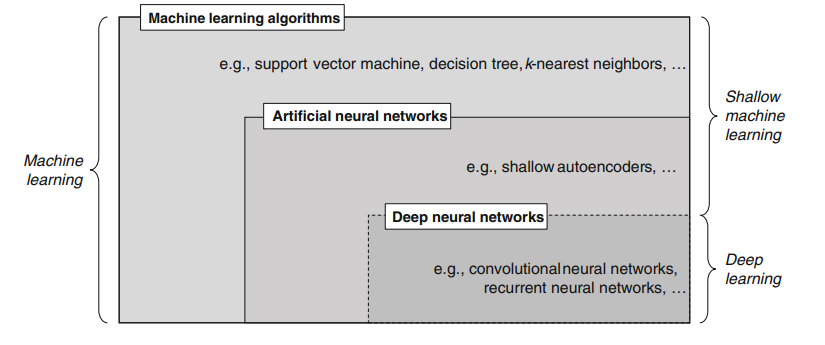
\includegraphics[width=0.8\textwidth,height=50mm]{./ml1.png}
	\end{center}
	\caption{Machine learning concepts \cite{Janiesch2021}.}
	\begin{center}
		\label{MLConcepts}
	\end{center}
\end{figure}


The concept of deep neural networks originates from biology, where a network of neurons is fundamental to the functionality of a brain. In overly simplified terms, such network consists of interconnected neurons that capture an external signal and produce a certain reaction within the brain as a response. Figure \ref{NeuronSchem} (a) illustrates a typical neuron, where the signal flows from dendrites through the cell-body of the neuron. If the signal is strong enough, the neuron activated and passes the signal further to other neurons through the connections called "synapses", as shown in Figure \ref{NeuronSchem} (c). Identical process takes place in remaining neurons, which ultimately forms a neural network \cite{Mehlig_2021}.

\begin{figure}[htb]
	\begin{center}
		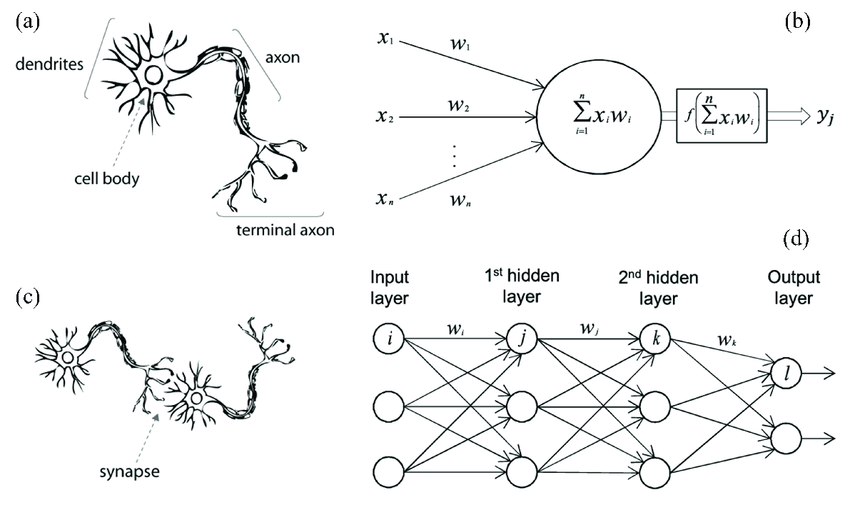
\includegraphics[height=8cm]{./BioNeuronVsArtificial.png}
	\end{center}
	\caption{A biological(a) neuron against artificial(b) and biological synapse(c) against artificial(d) \cite{article1}.}
	\begin{center}
		\label{NeuronSchem}
	\end{center}
\end{figure}

In deep learning(DL), a sub-field of ML, this architecture has been borrowed to implement an artificial neural network(ANN), where a neuron is simply a unit that processes an input signal. Figure \ref{NeuronSchem} (b) demonstrates a simplified structure of an artificial neuron. Here, $x_1, x_2..x_n$ represent input signals, while $\mathcal{W} = w_1, w_2, ... w_n$ are the weights of the signal and $y_i$ is the output of the neuron. The higher the weights of the input are, the stronger the influence of the neuron on the output. The weighted sum of the inputs is then passed to the activation function, which essentially determines the output of the node and ultimately allows to learn complex patterns in data \cite{Mehlig_2021}. 

A few of the most popular non-linear activation functions include a logistic sigmoid, tanh function, softmax and a rectified linear unit(ReLU). Among the four, ReLU has been considered state-of-the-art in the field of deep learning due to the performance in convolutional neural networks(CNN) \cite{Dubey2021} and the simplicity. The logic of ReLU can be represented as follows: 
  
\begin{equation}
	\operatorname{ReLU}(x)=\max (0, x)= \begin{cases}x, & \text { if } x \geq 0 \\ 0, & \text { otherwise }\end{cases}
\end{equation}

Consequently, the output of the activation function is passed to a hidden layer of neurons, as illustrated in Figure \ref{NeuronSchem} (d). The layers in the middle are called "hidden" due to the fact that both outputs and inputs are masked by the activation function.  The hidden layers will calculate the weighted output of the previous layers until the signal eventually reaches the final output layer of the network. Hidden layers that stack up together to form a classical deep learning architecture \cite{OShea2015}. Such architecture allows to process data in a non-linear pattern. In the original ANN all the layers are fully-connected(FC), meaning that each node of the input vector affects each node of the output vector, as shown in Figure \ref{NeuronSchem} (d).


Due to the biological nature, neural networks adapt over time by creating new connections between neurons. The neurons in ANN adopted such behaviour by utilizing a backpropogation algorithm \cite{Rumelhart:1986we}. A naive backpropogation approach is illustrated in Figure \ref{fig:backprop}. The algorithm consists of two parts: feed-forward and backward loops. Generally, the main objective of an ANN is to choose such weights that the network produces desired target outputs. The forward pass propagates along the nodes in each layer of the neural network and returns a predicted output. In order to evaluate the quality of the predicted output, it is compared to the target output by using a cost(loss) function. The classic example of a cost function is a mean-squared error (MSE), which is commonly used in regression based problems. The equation to MSE is shown in Equation \ref{MSE_eq}.

\begin{equation}\label{MSE_eq} 
{\operatorname{argmin}} \frac{1}{n} \sum_{i=1}^{n}\left(f\left(x_{i}\right)-y_{i}\right)^{2}
\end{equation}

The MSE cost function attempts to minimize the distance between the predicted output and the target output, while giving more weight to larger distances due to the squared output \cite{Albarghouthi2021}.


\begin{figure}[htb]
    \centering
    \subfloat{{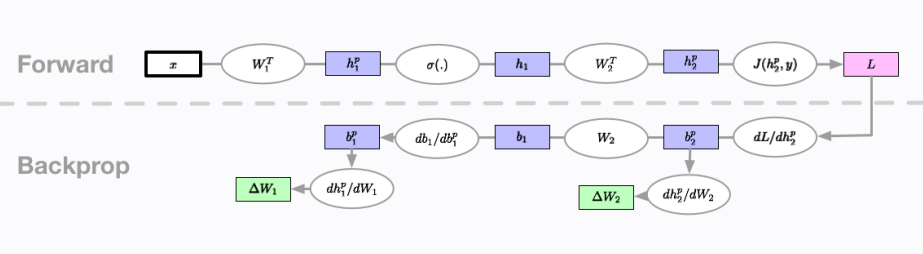
\includegraphics[width=10.5cm]{./Backprop1.png} }}%
    \qquad
    \subfloat{{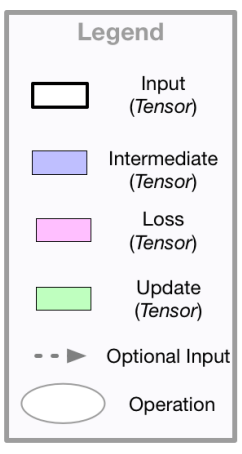
\includegraphics[width=1.5cm]{./Backprop2.png} }}%
    \caption{Backpropogation algorithm, adapted from \cite{Alber2018}.}\label{fig:backprop}%
\end{figure}

In order to minimize the loss function, the algorithm calculates the partial derivative of the loss term $\mathcal{L}$ with respect to the weights: $\nabla g = \frac{\partial \mathcal{L}(f(x_i), y_i)}{\partial \mathcal{W}}$. The basic algorithm of the gradient descent is commonly used in optimizing such functions and its logic can be generalized as follows: 

\begin{enumerate}
  \item Initialize the algorithm with a random value of $\theta^{i}$, where starts with $i=0$.
  \item Define the next $\theta$ value as $\theta^{i+1} = \theta^{i}-\eta\left((\nabla g)\left(\theta^{i}\right)\right)$.
  \item Iterate over the values of $i$ and repeat until convergence \cite{Albarghouthi2021}.
\end{enumerate} 

Generally speaking, there are three gradient descent algorithms: batch gradient descent, stochastic gradient descent(SGD) and mini-batch gradient descent. While the batch gradient descent updates the model only after all the samples have been evaluated, the SGD calculates the error for one sample in the dataset and updates the parameters one by one. On the other hand, the mini-batch gradient descent algorithm splits the data into smaller batches and calculates updates on each of the data subsets. 

Finally, by applying the chain rule to the derivatives in a backwards-direction, the updates for the matrix $\mathcal{W}$ are calculated for the nodes in the neural network \cite{Alber2018}. The algorithm is then repeated until the global minimum is reached. The process of determining the weight values to utilize in each subsequent layer in the neural network by means of backpropogation algorithm is called "training the model". During training, the value that $\Delta W$ are updated is known as "learning rate" (LR). This hyperparameter of the network typically equals to a small value between 0 and 1. Picking too high LR value would result in overshooting e.g. never finding the global minimum, while too low value will lead to slow convergence and higher computational costs. 

\FloatBarrier

\subsection{Neural networks in computer vision}
\label{neural_nets} 
With the discovery of DNN, many of the popular computer vision techniques became obsolete. Specifically, the introduction of CNNs was an important milestone in boosting machine perception performance \cite{Mahony2019}. Nowadays, CNNs are typically used to address various pattern recognition and computer vision tasks. Some of the tasks  include:

\begin{itemize}
	\item Image Classification
	\item Object Detection
	\item Segmentation
	\item Facial Recognition
	\item Domain Adaptation
	\item Image Reconstruction
	\item and many others \cite{paperswithcode:2022}
\end{itemize}

For addressing the key objectives of this work (Section \ref{objective}), the thesis will extensively cover image classification, object detection and domain adaptation tasks. Figure \ref{CNN} illustrates a simplistic CNN architecture approach to the MNIST  \cite{lecun-mnisthandwrittendigit-2010} classification problem. A CNN is essentially a neural network that leverages convolutional layers to produce predictions. Unlike the traditional computer vision methods, CNNs do not need to extract features of the image beforehand due to the logic behind convolution. In classical ML the features are extracted separately, followed by the appropriate algorithms for learning. On the contrary, DL algorithms, such as CNN, learn the features automatically \cite{alom01}.


\begin{figure}[htb]
	\begin{center}
		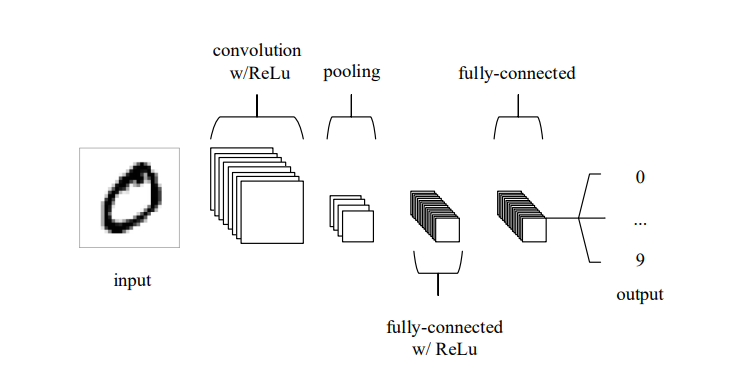
\includegraphics[height=5cm]{./CNN.png}
	\end{center}
	\caption{A simple CNN network with 5 layers for image classification task \cite{Mahony2019}.}
	\begin{center}
		\label{CNN}
	\end{center}
\end{figure}

To understand the logic behind convolutional layers, it is important to discuss the operation of convolution. Convolution is a mathematical operation of two functions that indicates how the shape of one is affected by another. In terms of image processing, convolution is a process, where the kernel moves along the input matrix dimensions. Each output pixel can then be calculated as the dot product of the cropped input and the kernel \cite{Liu2016}. Figure \ref{CNN_1} (a) illustrates the process of convolution in image processing.  
\begin{figure}[htb]
	\begin{center}
		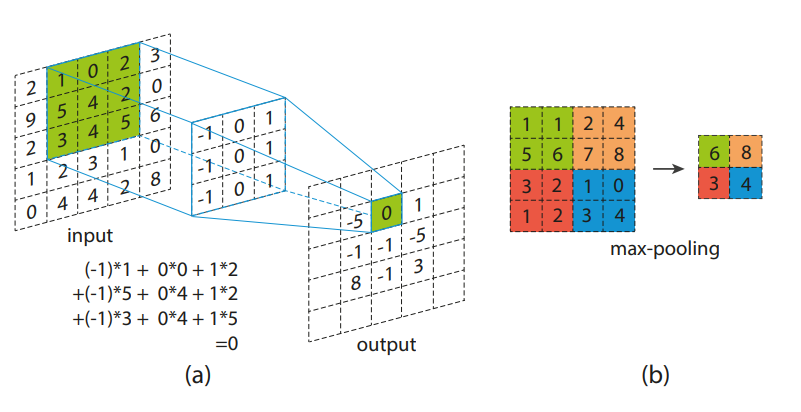
\includegraphics[height=5cm]{./CNN_1.png}
	\end{center}
	\caption{The process of convolution \cite{Liu2016}.}
	\begin{center}
		\label{CNN_1}
	\end{center}
\end{figure}

As a result, the elements of the network  are not densely connected, which allows better generalization and flexibility. This operation in practice allows to extract the important features of the image, such as edges, corners, shapes and many others.  However, unlike in the FC layers, the number of weights is much smaller, which is essential when it comes to high-dimensional images. Following the architecture in Figure \ref{CNN}, the outputs of the convolutional layers are activated with ReLU in a similar manner as in a classical ANN structure. The outputs are then pooled in order to down-sample the image and hence reduce the computational costs \cite{Liu2016}. The commonly used max-pooling operation is shown in Figure \ref{CNN_1} (b). Max-pooling down-samples the image by applying a filter that extracts the maximum value from the region of a feature map. Finally, fully-connected layers complete the structure of the basic CNN. FC layers are used to flatten the outputs from the convolutional layers. In case of the input in Figure \ref{CNN}, this in turn allowed to compute the probability of the input image to represent a number between 0 and 9 \cite{Mahony2019}.

CNNs boosted the performance in computer vision tasks. However, deep learning methods still required extensive training data. Luckily, multiple algorithms emerged as large datasets became available, which were made public as different image classification challenges appeared. The  datasets commonly used in benchmarking are ImageNet \cite{Russakovsky2014}, PASCAL Visual Object Classes (VOC) \cite{Everingham10} and Common Objects in Context (COCO) \cite{Lin2014}. The algorithms that emerged as a result of these challenges will be discussed in the following section. 
\FloatBarrier

\subsection{Image classification}
\label{classification_section} 
It is important to understand the concepts of image classification before moving on to object detection principles. Among the three mentioned earlier, ImageNet was chosen to be a de-facto dataset for running benchmarks.  Different CNN-based models were proposed and some of the most popular models include LeNet \cite{lecun-gradientbased-learning-applied-1998}, AlexNet \cite{NIPS2012_c399862d}, VGGNet \cite{Simonyan2014} and Residual Neural Network(ResNet) \cite{He2015}. As it can be concluded from Figure \ref{image_net}, the classification error dropped lower than the error of the manual detection with the introduction of ResNet, thus approaching the theoretical limits. 

\begin{figure}[htb]
	\begin{center}
		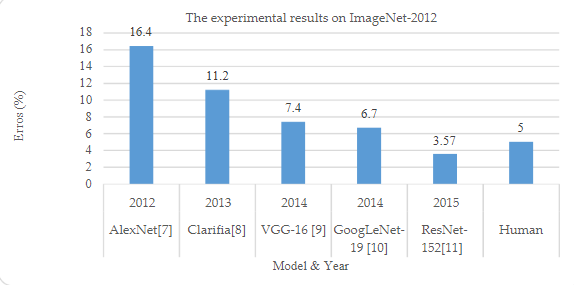
\includegraphics[height=5cm]{./image_net.png}
	\end{center}
	\caption{Evolution of image classifier models evaluated on ImageNet dataset \cite{alom01}.}
	\begin{center}
		\label{image_net}
	\end{center}
\end{figure}
\FloatBarrier

\subsubsection{LeNet}
LeNet architecture (1998) \cite{lecun-gradientbased-learning-applied-1998} is considered to be a pioneer in the field. Its design inherited the classic CNN architecture, but instead it consisted of 7 layers, as presented in Figure \ref{LeNet}. However, the implementation of the paper was not possible for more than 10 years due to limitations in computing power at the time. 

\begin{figure}[htb]
	\begin{center}
		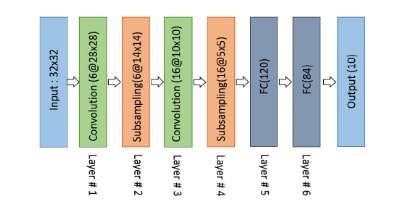
\includegraphics[height=4cm]{./LeNet.png}
	\end{center}
	\caption{LeNet architecture \cite{alom01}.}
	\begin{center}
		\label{LeNet}
	\end{center}
\end{figure}
\FloatBarrier

\subsubsection{AlexNet}
\label{alexnet_section} 
Consequently, AlexNet paper was introduced, which proved the effectiveness of their model, as it outperformed the state-of-the-art implementations and achieved the error rate of 15.3\% \cite{NIPS2012_c399862d}. Figure \ref{AlexNet} displays the proposed network. The architecture of AlexNet is similar to one of LeNet, though it is substantially deeper and has more than 60 million adjustable parameters. It has 5 convolutional layers of varying kernel size. The convolutional layers are followed byt ReLU activation functions and max-pooling layers. The architecture is finalized by attaching two FC layers with dropout rate of 0.5 and one softmax layer.

During dropout, there is a probability that the neuron will be excluded from computations in the subsequent layer. Utilizing such technique proved to be essential to fight over-fitting in FC layers and improve generalization  \cite{JMLR:v15:srivastava14a}. 

AlexNet architecture was the first CNN to split the model into two parts and to leverage mulitple GPUs in training due to GPU memory limitations of 3GB at the time \cite{NIPS2012_c399862d}. 

\begin{figure}[htb]
	\begin{center}
		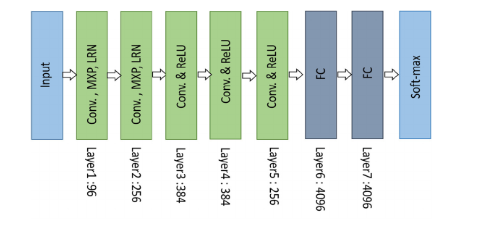
\includegraphics[height=4cm]{./AlexNet.png}
	\end{center}
	\caption{AlexNet architecture \cite{alom01}.}
	\begin{center}
		\label{AlexNet}
	\end{center}
\end{figure}
\FloatBarrier

\subsubsection{VGG}
Another milestone was achieved with the discovery proposed in VGGNet \cite{Simonyan2014}. This work proved that the depth of the network produces a significant impact on the performance of the CNN in classification tasks \cite{alom01}. Three different versions of the model were proposed with 11, 16 and 19 layers, respectively and with the deeper model being the best in performance, but more expensive in terms of computation. Equivalently to AlexNet, the network has blocks of convolutional layers of a mixed kernel size, followed by a ReLU block and max-pooling. The network is finalized with three FC and one softmax layers. 

\begin{figure}[htb]
	\begin{center}
		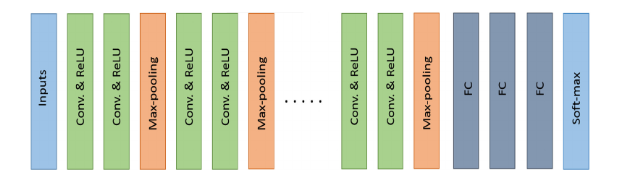
\includegraphics[height=4cm]{./vgg.png}
	\end{center}
	\caption{VGG architecture \cite{alom01}.}
	\begin{center}
		\label{VGG}
	\end{center}
\end{figure}
\FloatBarrier

\subsubsection{ResNet}
ResNet architecture \cite{He2015}, which was proposed in 2015, discovered that after reaching certain depth of the network, the performance of the model degrades. He et al. \cite{He2015} suggested that this happens due to the "vanishing gradient" problem. As the model gets deeper, several applications of the chain rule on during backpropogation tend to diminish either all the way to zero or becomes too large. As a result, no update is applied on the weights and hence, no training takes place. He et al. proposed to utilize a residual block, illustrated in Figure \ref{resnet}, which is used to skip some of the layers in between.  This solution essentially mitigates the problem of vanishing gradients by allowing the training loop to skip parts of the network that negatively affect the performance.

\begin{figure}[htb]
	\begin{center}
		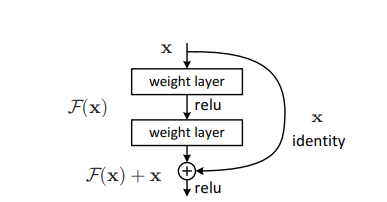
\includegraphics[height=4cm]{./resnet.png}
	\end{center}
	\caption{Residual block of ResNet \cite{He2015}.}
	\begin{center}
		\label{resnet}
	\end{center}
\end{figure}

ResNet adopts the VGG-19 architecture, but adds a skip connection block. He et al. implemented multiple versions of the model and the largest one is 152 layers deep. Nonetheless, the network has less trainable parameters than VGG, which substantially improves the training speed while preserving accuracy due to the residual block. As a result, the proposed model achieved the error of 3.57\% on ImageNet dataset, which is lower than the human eye error \cite{He2015}.

\begin{figure}[htb]
	\begin{center}
		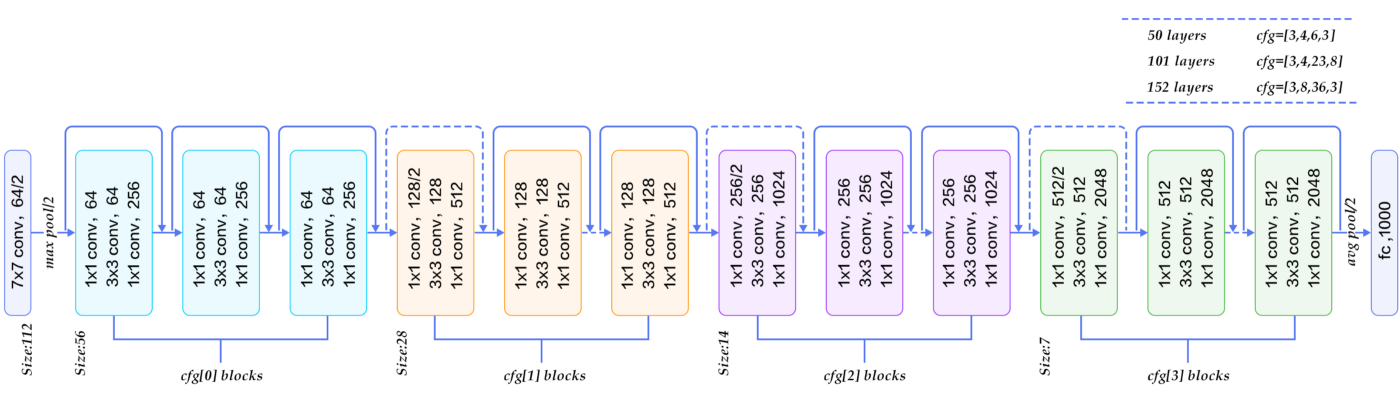
\includegraphics[width=16cm]{./resnetFull.png}
	\end{center}
	\caption{ResNet architecture \cite{resnet50}.}
	\begin{center}
		\label{resnetFull}
	\end{center}
\end{figure}
\FloatBarrier


\subsection{Object detection}
\label{obj_detection_section} 
The problem of object detection is an extended version of the image classification problem. However, unlike image classification, object detection aims to recognize not only the object, but also to localize it. Prior to arrival of deep learning, object detection considered to be a difficult task. With the discovery of the CNN architecture, the traditional computer vision techniques became obsolete. Since then, multiple different detector algorithms emerged. A typical object detection network contains two important modules - the base (or backbone) network  and the detector network. A base network is usually one of the pre-trained VGG or ResNet models, presented in the previous chapter. A base network acts as a feature extractor, and the features are then passed to a detector. Generally speaking, deep learning based detector networks can be classified into two categories: single- and two-stage detectors \cite{Zaidi2021}, as shown in Figure \ref{OD}.  

\begin{figure}[htb]
	\begin{center}
		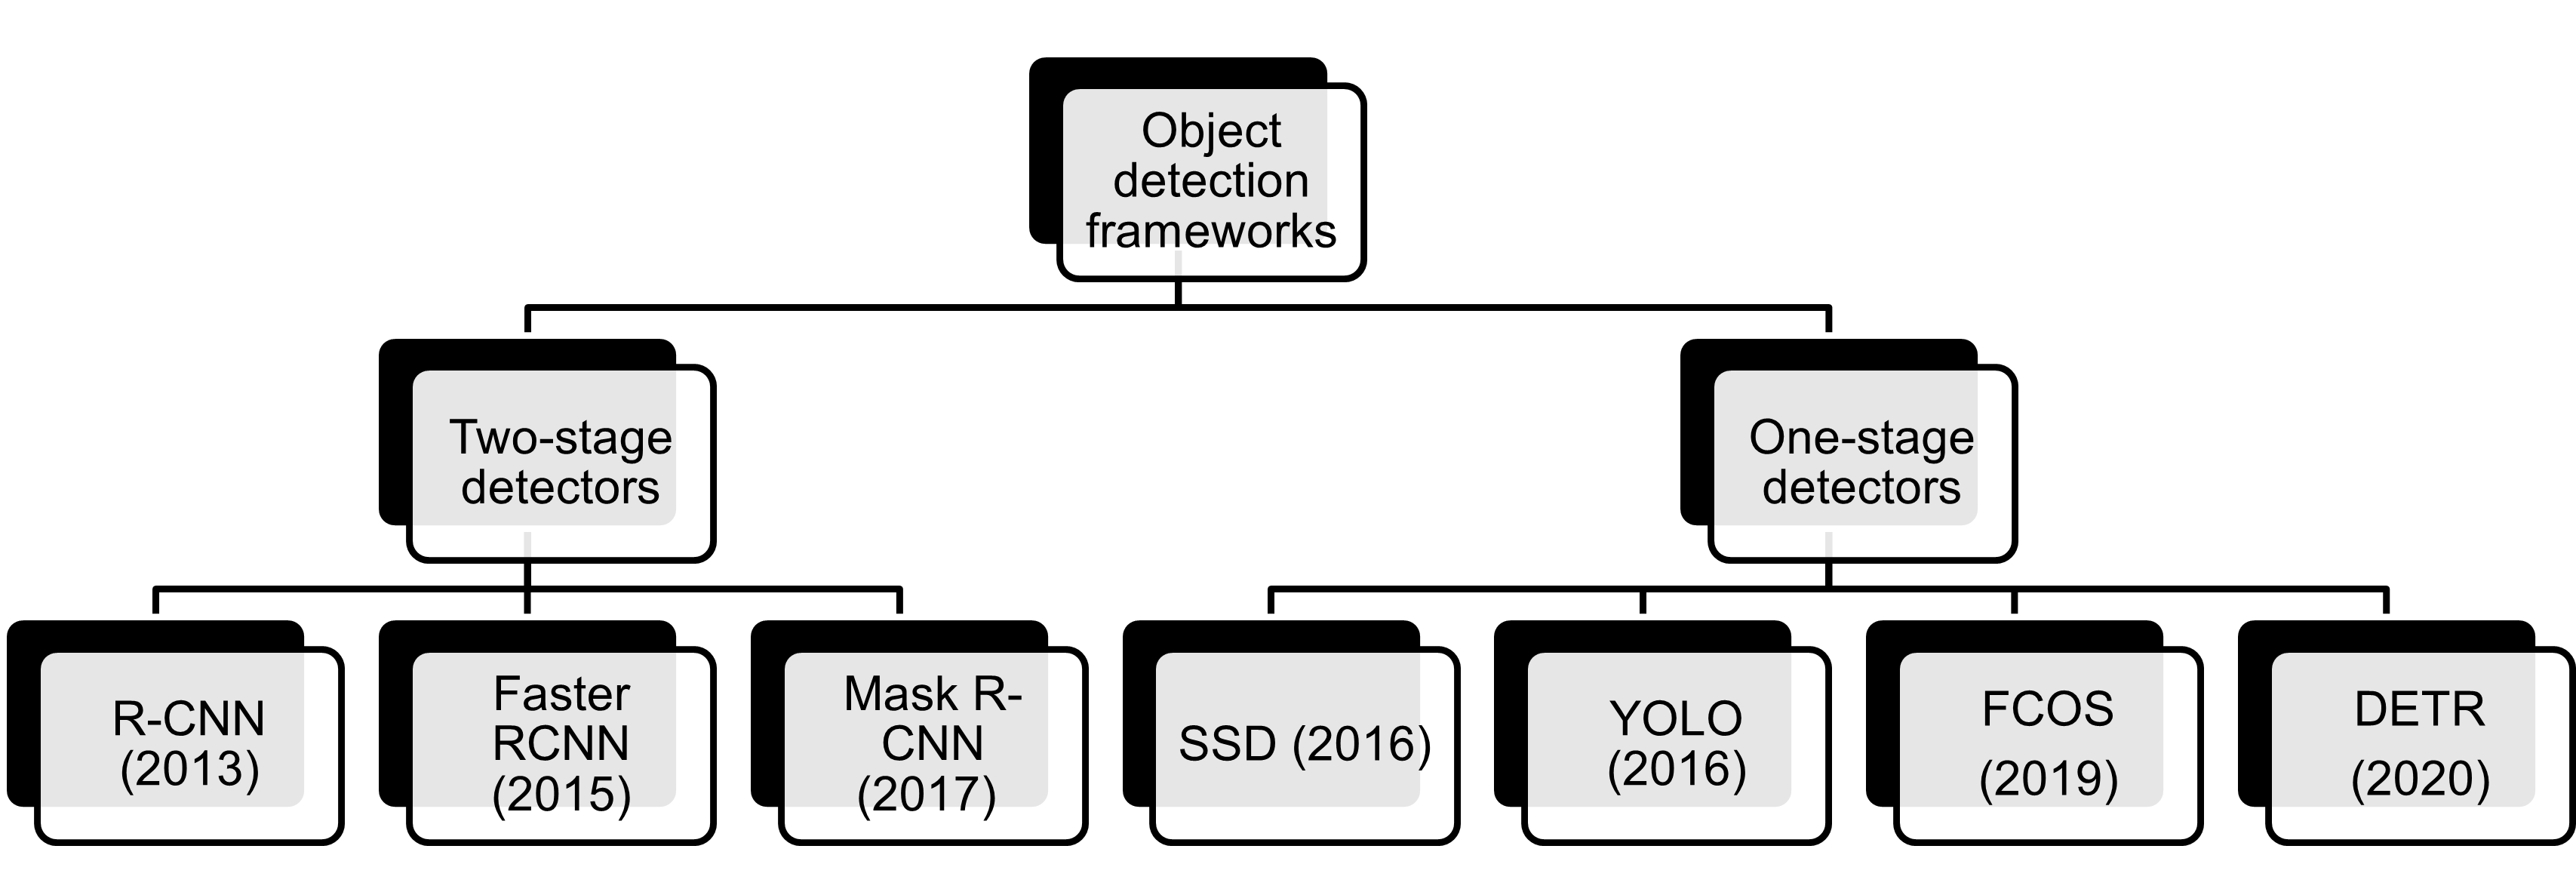
\includegraphics[width=16cm]{./OD.png}
	\end{center}
	\caption{Types of object detectors.}
	\begin{center}
		\label{OD}
	\end{center}
\end{figure}

Two-stage object detectors attempt to propose regions of the image that contain an object first, and then run the task of classification and localization on the proposed region. On the other hand, single-stage detectors try to detect objects directly without running the  Region Proposal Network (RPN). Figure \ref{fig:1vs2stage} illustrates the key differences in the architecture.

\begin{figure}[htb]
    \centering
    \subfloat{\raisebox{0.13\height}{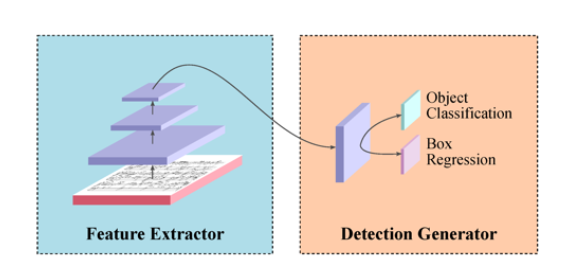
\includegraphics[width=6cm]{./1stage.png} }}%
    \qquad
    \subfloat{{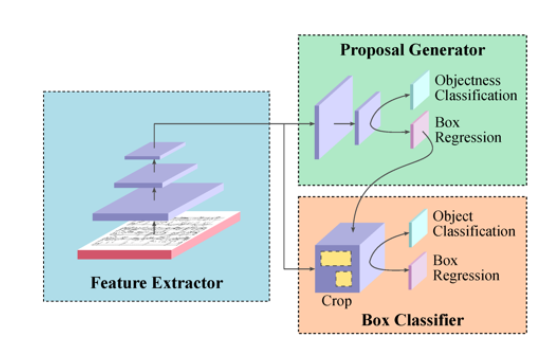
\includegraphics[width=6cm]{./2stage.png} }}%
    \caption{A simple single-stage detector(left) compared to a two-stage detector(right) \cite{app8091488}.}\label{fig:1vs2stage}%
\end{figure}

Typical examples of the single-stage networks are RetinaNet \cite{Lin2017}, Single-shot detector(SSD) \cite{Liu2015} and You Only Look Once(YOLO) \cite{Redmon2015a}. In two-stage detectors, Region-based CNN(R-CNN) \cite{Girshick2013}, Fast-RCNN \cite{Girshick2015} and Faster-RCNN \cite{ima} are considered to be the most important discoveries. Figure \ref{OD} also mentions detectors such as FCOS \cite{Tian2019}, Mask-RCNN \cite{He2017} and DETR \cite{Carion2020}. Although they show competitive performance, they are not reviewed in the thesis as they are not relevant to the method introduced in the \nameref{Methodology}.  The following subsection will introduce the reader to some of the main concepts of the selected detectors. 

\FloatBarrier

\subsubsection{R-CNN}

Figure \ref{rcnn} shows the structure of the R-CNN network \cite{Girshick2013}. R-CNN has been one of the first CNN-based models to be introduced \cite{Zaidi2021}. Girshick et al. essentially suggested to use a module that extracts the object proposals and then to pass it to a CNN. The CNN would then extract the features relevant, which would in turn allow to classify the proposed region as well as to localize it. In their original experiments, the selective search algorithm  \cite{Uijlings13} was used to produce roughly 2000 regions. AlexNet  \cite{NIPS2012_c399862d} was used as a backbone CNN to extract vectors of 4096 size dimensions. The features were then passed to binary classifiers that are bound to a certain class. As multiple regions are returned, non-maximum suppression(NMS) \cite{Hosang2017}  is used to identify the best proposal for the object. 

Unfortunately, the inference process in R-CNN took a whole 47 seconds per image \cite{Girshick2013}, which was not fast enough to be remain relevant in the object detection field. 

\begin{figure}[htb]
	\begin{center}
		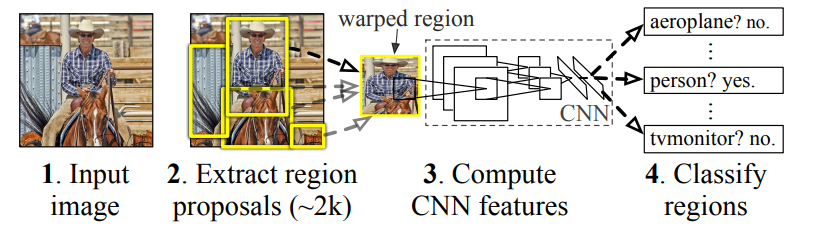
\includegraphics[width=12cm]{./rcnn.png}
	\end{center}
	\caption{R-CNN overview \cite{Girshick2013}.}
	\begin{center}
		\label{rcnn}
	\end{center}
\end{figure}
\FloatBarrier


\subsubsection{Fast-RCNN}
Unlike the classic R-CNN system, where the components such as the classifier and the regressor have to be trained separately, the same authors of the RCNN  model also introduced a Fast-RCNN model \cite{Girshick2015}, which proposed an end-to-end trainable system. Additionally, the Region-of-Interest (ROI) pooling layer was proposed. This ROI component essentially divides the image into a grid of a fixed size and applies average pooling. The resulted one-level pyramid of the image is used as a feature map for the detector head. This allows the rest of the network to focus purely on the features extracted for the proposed regions. Finally, two additional FC output layers are appended, where the first one classifies the features by returning the probability of N object classes in range $(0, N+1]$, which includes the background class as well. The other one returns a vector of a size $(0, 4\times N]$, thus including the bounding box coordinates for the foreground classes only \cite{Girshick2015}. Fast-RCNN showed a significant($\times 146$) speed improvement as compared to the R-CNN, thus allowing it to be used in real-time applications \cite{Girshick2013}. The original architecture of Fast-RCNN is shown in Figure \ref{fast_rcnn} below. 

\begin{figure}[htb]
	\begin{center}
		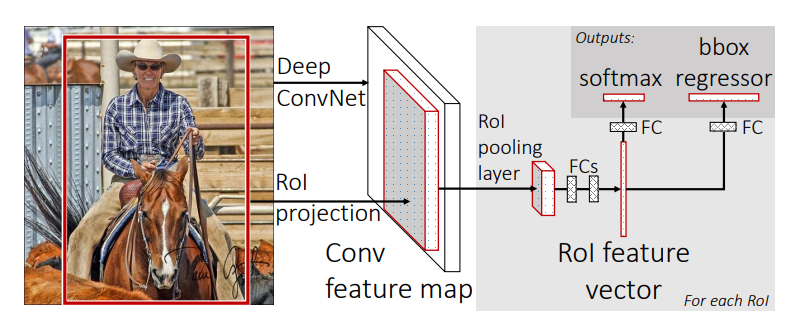
\includegraphics[width=10cm]{./fast_rcnn.png}
	\end{center}
	\caption{Fast-RCNN overview \cite{Girshick2015}.}\label{fast_rcnn}
	\begin{center}
	\end{center}
\end{figure}
\FloatBarrier

\subsubsection{Faster-RCNN} 
Ren et al. \cite{ima} discovered that even though Fast-RCNN was significantly faster than the preceding networks, the region proposing process was still causing a bottleneck. Therefore, in the novel Faster-RCNN \cite{ima} architecture it was suggested to replace the legacy region proposal module with a fully-convoluted architecture called region proposal network(RPN) \cite{Girshick2013}. Instead of using the one-level image pyramid to solve the problem as it was proposed by Girshick et al. \cite{Girshick2015}, Faster-RCNN utilizes anchor boxes of different aspect ratios to propose object candidates. Similarly to any other CNN, the features in Faster-RCNN are extracted from the convolutional layers based on a VGG backbone. The features maps are then sent to the RPN, which in practice is a sliding window  of $n\times n$ $(n=3)$ dimensions. At every sliding window position, the $k$ number of object proposals are predicted. Such boxes are called "anchors" as illustrated in Figure \ref{fig:faster_rcnn}. The acquired $2k$ classification predictions whether the proposed region is an object of interest or not and $4$ regression outputs of the bounding box coordinates are then mapped back to the ROI layer and, eventually, to the FC layers that predict the class of the proposed object \cite{ima}. 


\begin{figure}[htb]
    \centering
    \subfloat{{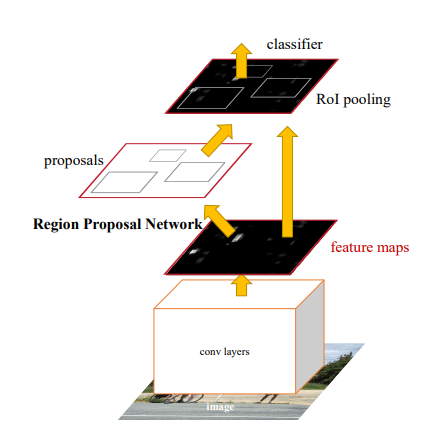
\includegraphics[width=6cm]{./faster_rcnn.png} }}%
    \qquad
    \subfloat{\raisebox{0.5\height}{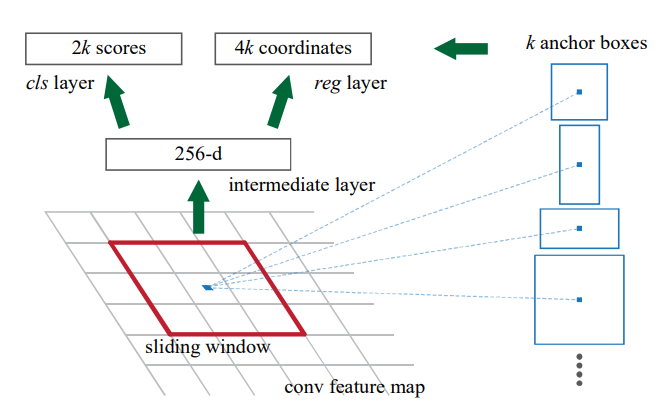
\includegraphics[width=6cm]{./faster_rcnn_rpn.png} }}%
    \caption{Faster-RCNN overview and its RPN module \cite{ima}.}
    \label{fig:faster_rcnn}%
\end{figure}

As the network returns the predictions, the loss function is as follows:  
\begin{equation}
\begin{array}{r}
L\left(\left\{p_{i}\right\},\left\{t_{i}\right\}\right)=\frac{1}{N_{c l s}} \sum_{i} L_{c l s}\left(p_{i}, p_{i}^{*}\right) + \lambda \frac{1}{N_{\text {reg }}} \sum_{i} p_{i}^{*} L_{r e g}\left(t_{i}, t_{i}^{*}\right)
\end{array},
\label{faster_rcnn_loss} 
\end{equation}

where $p_i$ is the probability of the predicted anchor $i$ to be an object,  $p_{i}^{*}$ is a ground-truth label from 0 to 1, $t_i$ is a vector with 4 coordinates of the bounding box and $t_{i}^{*}$ is its corresponding ground-truth vector. $\lambda$ is a trade-off between the $L_{cls}$ and $L_{reg}$, where $L_{c l s}$ is calculated as a binary log loss and $L_{reg}$ uses a smooth $L_1$ loss that was introduced in Fast-RCNN \cite{Girshick2015}.  




This implementation, unlike Fast-RCNN, allowed to return predictions nearly in real time with the breakthrough of 5 frames per second(FPS) \cite{ima}.
Although the two-stage Faster-RCNN detector is nearly 7 years old at the time of writing this thesis, it is still one of the most widely used detectors in the field, as can be noticed from Figure \ref{popularity}. In later chapters, this work will focus on the Faster-RCNN implementation. Nevertheless, it is worth mentioning single-stage competitors. Often they are slightly weaker in terms of accuracy, compared to two-stage detectors. However, these detectors offer a significant improvement in robustness as compared even to the fastest one of the two-stage detectors, Faster-RCNN. 

\begin{figure}[htb]
	\begin{center}
		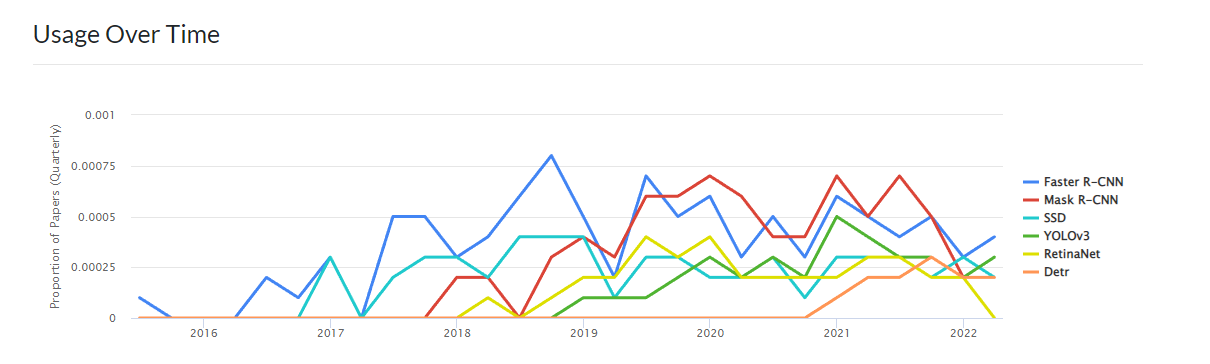
\includegraphics[width=14cm]{./detectorsPopularity.png}
	\end{center}
	\caption{The popularity of different detectors according to  \cite{paperswithcode_1:2022}.}
	\begin{center}
		\label{popularity}
	\end{center}
\end{figure}

\FloatBarrier

\subsubsection{YOLO}
\label{yolo_section} 

Unlike the two-stage methods presented, You Only Look Once(YOLO) \cite{Redmon2015a} algorithm attempts to solve the object detection problem purely as a regression problem by predicting the bounding boxes of the objects directly without region proposals. The YOLO network instead splits the image into a grid of $S\times S$ cells, for which a $B$ number of bounding boxes and $C$ probabilities of the class and  are predicted \cite{Redmon2015a}. The overview of the detection process is shown in Figure \ref{yolo}. The principle of the YOLO grid component is broadly similar the one of R-CNN \cite{Girshick2013}, where the algorithm of selective search \cite{Uijlings13} is used to propose regions. However, instead of proposing more than 2000 regions, YOLO only returns 98 proposal boxes per image. This, along with having an optimized single-stage detection process, allowed YOLO to achieve impressive nearly real-time FPS results. Redmon et al. reported YOLO to sustain the average FPS of 45, while the most accurate version of the Faster-RCNN network had 7 FPS \cite{Redmon2015a}. However, the proposed network still has multiple limitations, which were addressed in later iterations of the paper  \cite{Redmon2016, Redmon2018a}.

The architecture consists of 24 cascaded convolutional and 2 FC layers. The convolutional layers are first pre-trained on the ImageNet dataset \cite{Russakovsky2014}. The image size is reduced by applying $1\times1$ convolutional layers in between, also referred to as "reduction layers"  \cite{Redmon2015a}. The simplified architecture is presented in Figure \ref{ssd}.

\begin{figure}[htb]
	\begin{center}
		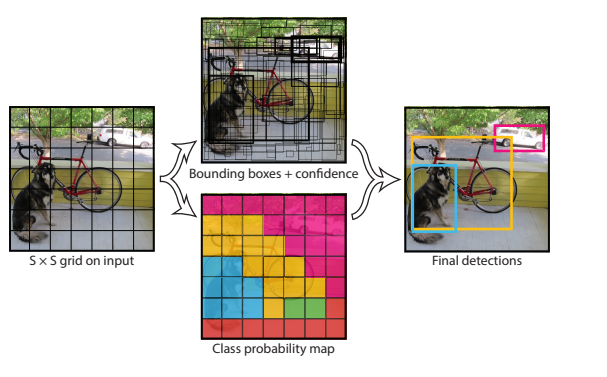
\includegraphics[width=12cm]{./yolo.png}
	\end{center}
	\caption{YOLO overview \cite{Redmon2015a}.}
	\begin{center}
		\label{yolo}
	\end{center}
\end{figure}
\FloatBarrier


%%\subsubsection{RetinaNet}

%%\begin{figure}[htb]
%%	\begin{center}
%%		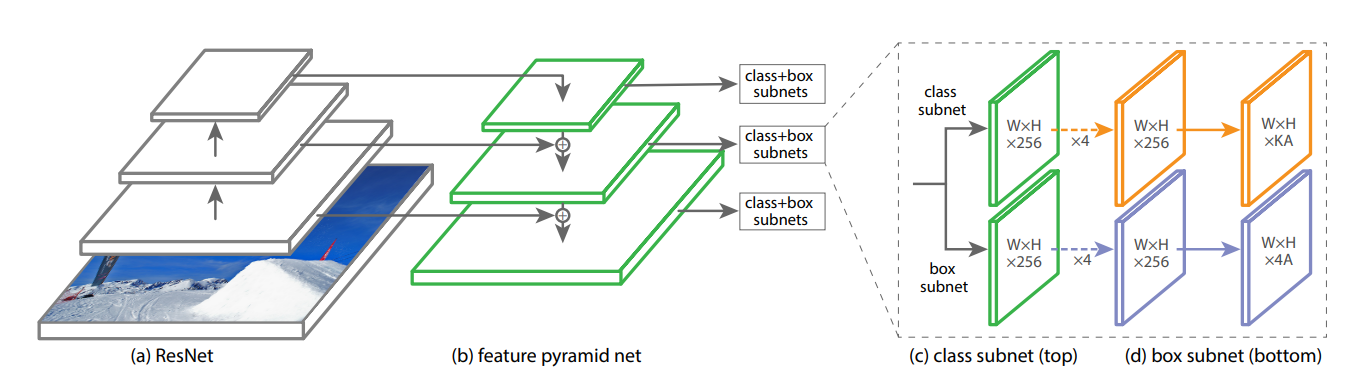
\includegraphics[width=14cm]{./retinaNet.png}
%%	\end{center}
%%	\caption{RetinaNet overview\cite{Lin2017}}
%%	\begin{center}
%%		\label{retinanet}
%%	\end{center}
%%\end{figure}
%%\FloatBarrier


\subsubsection{SSD}
Another implementation of a single-stage network worth mentioning is a Single-Shot MultiBox detector(SSD) \cite{Liu2015}. The differences in architectures of SSD and YOLO are displayed in Figure \ref{ssd}. Liu et al. proposed a model that detects objects in real-time while preserving the accuracy. First, the image is fed into the backbone CNN, in the original experiments - VGG-16. The SSD head layers added after the backbone network are convolutional as well. Similarly to YOLO, the image is split into a grid of $n\times n$ size, where it benefits from the anchor boxes of varying aspect ratio. 


\begin{figure}[htb]
	\begin{center}
		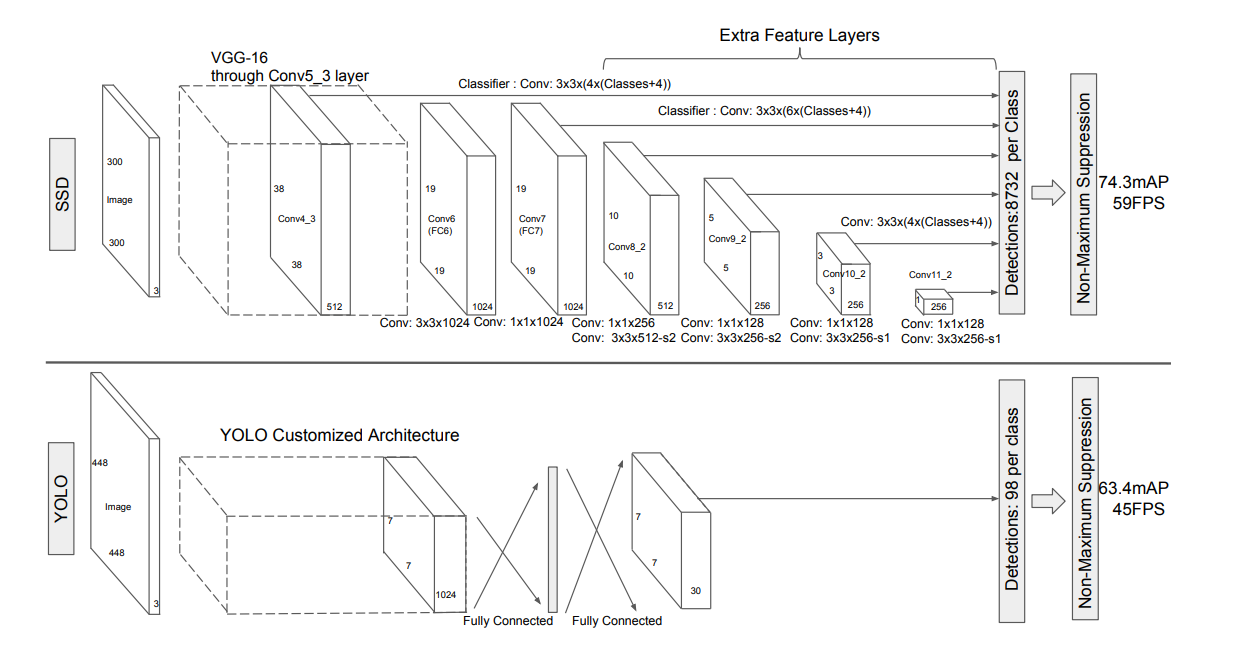
\includegraphics[width=14cm]{./ssd_yolo.png}
	\end{center}
	\caption{SSD compared to YOLO \cite{Liu2015}.}
	\begin{center}
		\label{ssd}
	\end{center}
\end{figure}

However, as the objects might not always be within the grid boundaries, as can be noticed from Figure \ref{ssd_boxes}. Therefore, SSD paper introduced a concept of anchor boxes with offsets. The anchor boxes with offsets that have the highest overlap with the ground truth box of the object are then passed to FC layers to predict the class and the location of the object. 

\begin{figure}[htb]
	\begin{center}
		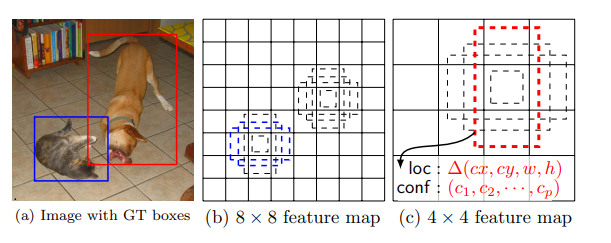
\includegraphics[width=12cm]{./ssd_boxes.png}
	\end{center}
	\caption{SSD anchor boxes \cite{Liu2015}.}
	\begin{center}
		\label{ssd_boxes}
	\end{center}
\end{figure}
\FloatBarrier

The key object detection models of the last decade are presented in Table \ref{detectorsTable} below. As it can be deducted from Table, Faster-RCNN shows the best performance on the PASCAL VOC dataset, while YOLO demonstrated the highest FPS. The survey of Zaidi et al. \cite{Zaidi2021} also discusses lightweight models. However, for the purpose of this study, the detection accuracy is the primary focus rather than speed, thus their review will be omitted. 

\begin{table}[htb]
	\captionof{table}{Overview of object detectors \cite{Zaidi2021}. }
	\begin{center}
		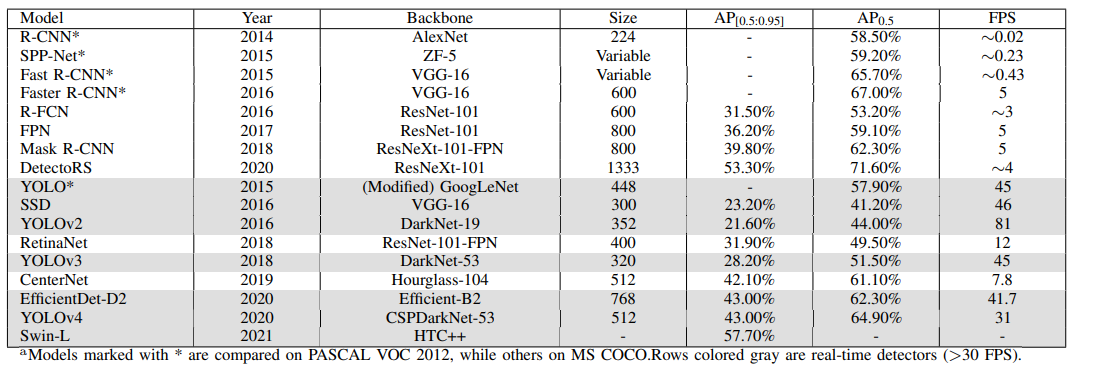
\includegraphics[width=16cm]{./detectorsTable.png}
	\end{center}
	\begin{center}
		\label{detectorsTable}
	\end{center}
\end{table}

As can be seen from Table \ref{detectorsTable}, there are multiple models that are not covered in this section. Additionally, there are several detectors that show promising results in the domain-adaptive object detection setup, such as FCOS \cite{Tian2019} and DETR \cite{Zhang2021b}. However, as their performance is not yet extensively evaluated, they will be omitted from this thesis. 
\FloatBarrier

\subsection{Object detection in industrial environments}
Although object detection is an extremely diverse field with applications varying from medicine \cite{9689485} to self-driving vehicles \cite{Janai2017, Shan2018}, the industrial object detection is mostly limited to safety and process monitoring \cite{Awalgaonkar2020, Banf2022}. Fewer research has addressed the topic of industrial object detection. In general, many of the introduced object detection methods can be applied to this problem directly as it is. Malburg et al. \cite{MALBURG2021581} has evaluated multiple different versions of object detection models such as YOLO \cite{Redmon2015a} in an industrial setup. However, often in industrial environments severe challenges such as overlapping and occlusion take place. Moreover, the object instances often are represented in multiple scales. Therefore, it is often impossible to obtain reliable results using a standard object detector architecture. Wu et al. \cite{Wu2022} has recently addressed the problem of industrial object detection using an R-CNN based approach that leverages Feature Pyramid Networks to improve detection at multiple scales and NMS with penalty factors to eliminate occlusion problem. However, the proposed method does not consider the data availability limitations and confidentiality issues that were outlined in the \nameref{objective}. On the other hand, Kim et al. \cite{Kim2020} minimized the need for labeling from a human by utilizing a deep active learning model. While the core of this approach is a standard Faster-RCNN \cite{ima} network, Kim et al. also proposed to utilize uncertainty evaluation in order to enable the model to label images interactively over time. As the training advances, the model evaluates whether the predicted bounding boxes are reliable or not using the sum of entropy for each bounding box. In the subsequent stage the model requests the user to manually label 10\% of the data with highest uncertainty. The model is then retrained with the updated knowledge. Although this approach seems promising, it  does not consider the domain shift phenomenon that takes place in the setup defined by the \nameref{objective}. Later sections of the thesis will address this phenomenon. 


\subsection{Transfer learning}
\label{transferLearning} 
In this section, multiple transfer learning(TL) techniques will be introduced. Despite the fact that the methods discussed in the previous chapters have been successfully implemented in various scenarios, ML in general often struggles to apply such methods in real life. This is normally caused by insufficient training data, as it is often expensive to collect it, both in terms of time, financially, and sometimes simply not possible at all due to data accessibility issues \cite{Zhuang2019}. Moreover, the requirement of having to train the models on new massive datasets often make ML solutions inefficient in practice. For this reason, TL concepts have been found advantageous as it addresses transferring knowledge learned from one task, domain or distribution to another. Here and in the subsequent sections, the notations are identical to those outlined by Pan et al. \cite{Pan2010} and are introduced as follows:  

\begin{itemize}
\item A domain $\mathcal{D}$ can be defined as a composite term, which is characterized by two elements: feature space $\mathcal{X}$ and a marginal probability distribution $P(X)$; $X=\left\{x_{1}, \ldots, x_{n}\right\} \in \mathcal{X}$. With this being said, two domains are defined as different if their feature spaces or marginal probability distributions are different. In this thesis, the domains are restricted with one source $\mathcal{D_S}$ and one target $\mathcal{D_T}$ domains \cite{Pan2010}. 
\item Similarly, a task $\mathcal{T}$ can be defined by its label space $\mathcal{Y}$ and a conditional probability of $\mathcal{Y}$ given $X$, e.g. $P(Y \mid X)$, $Y=\left\{y_{1}, \ldots, y_{n}\right\} \in \mathcal{Y}$. In practice, a conditional probability is defined as a function that can learn to predict a label $y_i$ given a sample vector $x_i$ \cite{Pan2010}. 
\end{itemize} 


 
\begin{figure}[htb]
	\begin{center}
		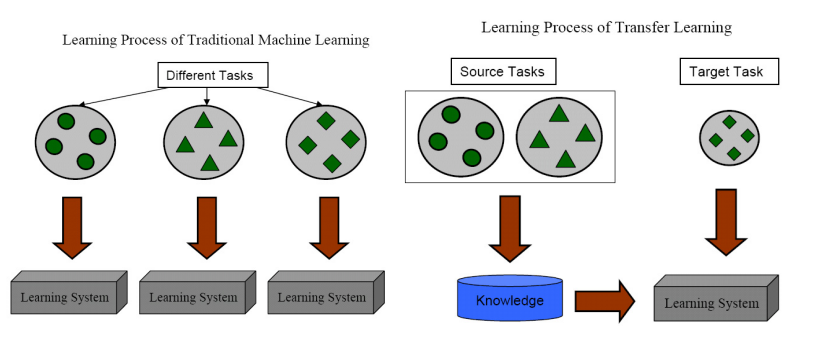
\includegraphics[width=16cm]{./TL.png}
	\end{center}
	\caption{Comparison of ML to TL \cite{Pan2010}.}
	\begin{center}
		\label{TL}
	\end{center}
\end{figure}

Sun et al. \cite{SUN201584} describes TL as a method to transfer knowledge when the feature space between the two given source and target domains is different, meaning that $\mathcal{X}_{S} \neq \mathcal{X}_{T}$. Pan et al. \cite{Pan2010} mentions that transfer learning can be also defined when the marginal probability is different, meaning that $P_{S}(X) \neq P_{T}(X)$. Similarly, transfer learning can be applied when $\mathcal{T}_{S} \neq \mathcal{T}_{T}$. An example of a simple TL problem is training a model that was trained for classifying cats, but instead is  required to learn a new task such as classifying dogs. However, in various scenarios, the task is essentially the same but the domain is similar yet different. For instance, a model that was trained to identify cats in sketches, is instead required to identify cats in real images. Solving such tasks is the main focus of domain adaptation(DA). Often the terms "domain adaptation" and "transfer learning" are used interchangeably. However, according to Wang et al. \cite{Wang2018} and Zhang et al. \cite{Zhang2021}, domain adaptation(DA) is a special case of TL. In scientific terms, the problem that DA attempts to solve can be defined when the source and target feature spaces are the same $\mathcal{X}_{S}=\mathcal{X}_{T}$, but the marginal probability distribution is not $P\left(\mathcal{X}_{S}\right) \neq P\left(\mathcal{X}_{T}\right)$ \cite{SUN201584}. This is not to be confused with semi-supervised machine learning, where both labeled and unlabeled data is typically supplied from one domain \cite{SUN201584}. 
\FloatBarrier

%https://www.v7labs.com/blog/transfer-learning-guide


\subsubsection{Domain adaptation}
\label{DA_section} 
Domain Adaptation (DA) has lately been gaining popularity in both image classification and object detection tasks \cite{Zhang2021}. Typically, DA is used to predict a label given the data from a source domain and limited or no data from the target domain. Most importantly, DA addresses the domain shift problem \cite{Zhang2021}. In a DA problem, a domain shift, also known as a distributional shift or dataset bias, can be defined as a change in distribution of data between source and target domains. 


Zhang et al. \cite{Zhang2021} classify DA methods into three categories that are similar to ML types - supervised, semi-supervised, and unsupervised DA. Alternatively, Oza et al. \cite{Oza2021} classify the collected DA methods into semi-supervised, weakly-supervised and unsupervised DA. Indeed, supervised DA is not commonly used since the primary goal of DA is to reduce the domain shift when the data availability is limited. 

According to Zhang et al. \cite{Zhang2021}, different methods that attempt to solve the distribution shift problem by minimizing the distance between marginal, conditional or joint distributions. 

The visual representation of these distribution alignment types are shown in Figure \ref{distribution} and the methods in the following subsections attempt to minimize the domain shift by one way or another. 

\begin{figure}[htb]
	\begin{center}
		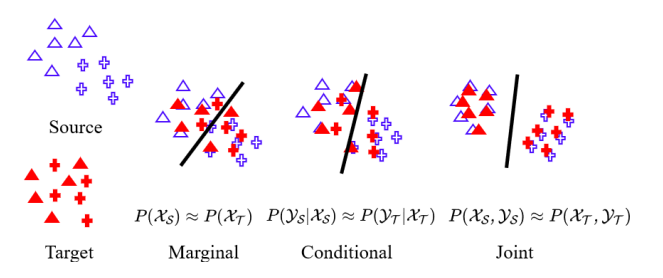
\includegraphics[width=12cm]{./distribution.png}
	\end{center}
	\caption{Distribution alignment types \cite{Zhang2021}.}
	\begin{center}
		\label{distribution}
	\end{center}
\end{figure}
\FloatBarrier 



\subsection{Domain-adaptive object detection}
\label{DAobj} 
Next subsection will discuss some of the methods that were proposed at different times to solve the problem of domain shift in object detectors. Oza et al.  \cite{Oza2021} have extensively reviewed and grouped the existing approaches into following six categories:
\begin{enumerate}
	\item Adversarial feature learning
	\item Pseudo-label based self-training
	\item Image-to-image translation
	\item Domain randomization 
	\item Mean-teacher training
	\item Graph reasoning
\end{enumerate} 

Many of the methods collected by Oza et al. overlap with each other and fall into more than one group. In this thesis, a few methods will be briefly reviewed for each of the categories above. Some of the methods are listed in Figure \ref{UDA_OD}.

\begin{figure}[htb]
	\begin{center}
		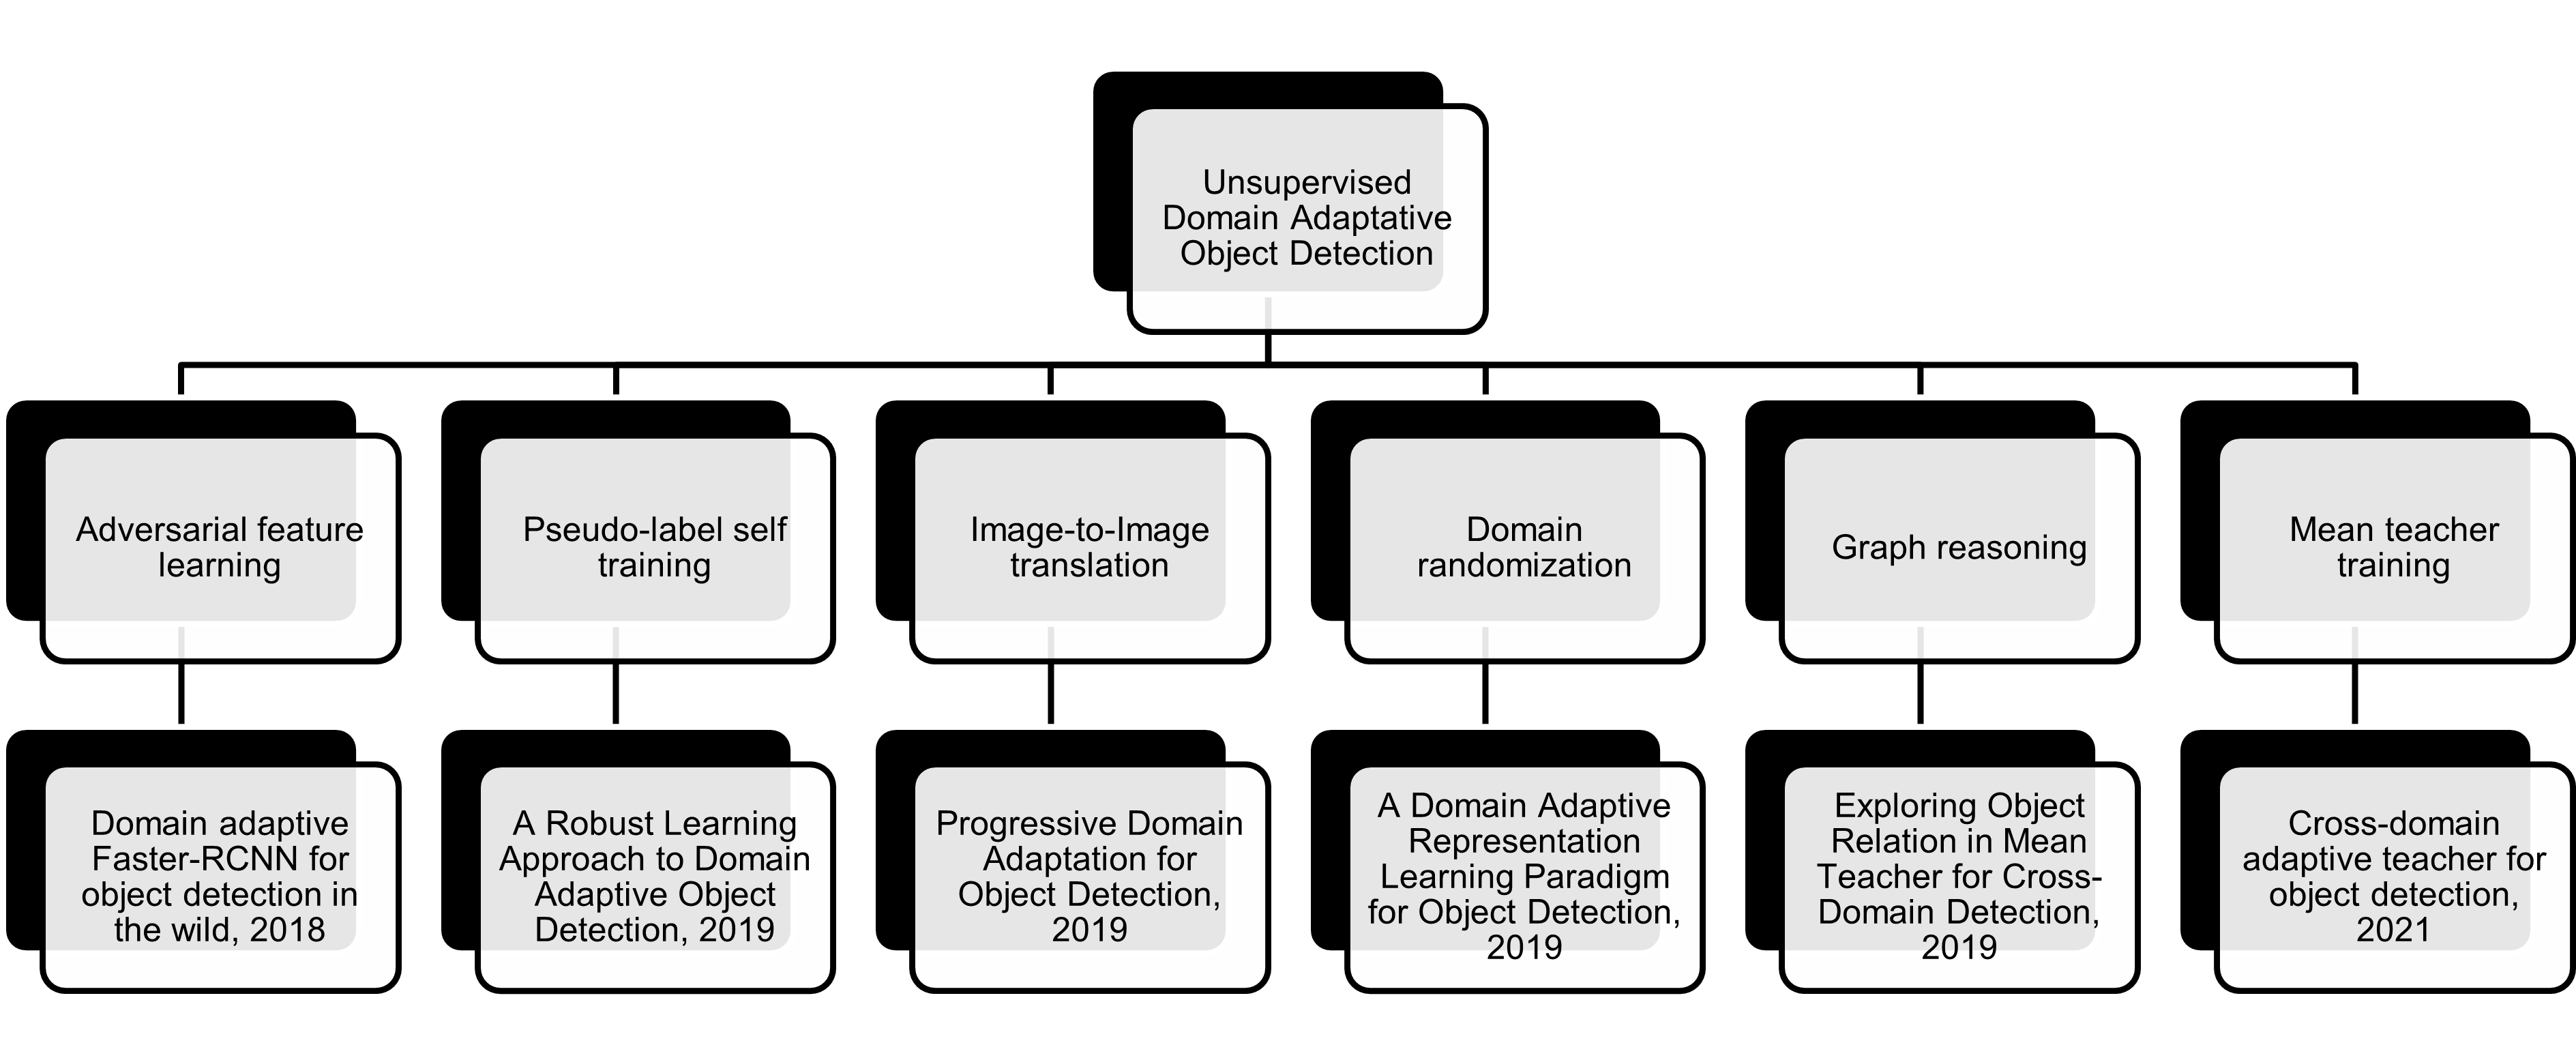
\includegraphics[width=16cm]{./UDA_OD.png}
	\end{center}
	\caption{Unsupervised Domain Adaptive Object Detection.}
	\begin{center}
		\label{UDA_OD}
	\end{center}
\end{figure}

In the following methods, it will be assumed that $\mathcal{D_S}$ and $\mathcal{D_T}$ originate from similar yet different distributions. Additionally, the papers introduced in the following section address unsupervised domain adaptation(UDA) problem, which is naturally more sophisticated than a supervised DA.
\FloatBarrier

\subsubsection{Gradient reversal layer}

One of the key components in a typical domain adaptive setup for both image classification and object detection problems is a gradient reversal layer (GRL) that has been proposed by Ganin et al. \cite{Ganin2015}. The authors suggest that in order to successfully solve the domain adaptation problem, the prediction should be based on the features that are as indistinguishable as possible  between the source and target domains. In other words, the network should propose features that are common for both domains. Figure \ref{DANN} illustrates the Domain-Adversarial Neural Network (DANN) proposed by Ganin et al. \cite{Ganin2015}. 

\begin{figure}[htb]
	\begin{center}
		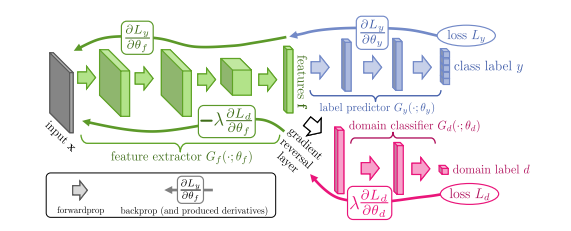
\includegraphics[width=16cm]{./GRL.png}
	\end{center}
	\caption{Domain-adversarial neural network and GRL \cite{Ganin2015}.}
	\begin{center}
		\label{DANN}
	\end{center}
\end{figure}

The network is essentially a simple feed-forward network with a feature extractor and a predictor that classifies the input image. Two additional components are appended to the last layer of the feature extractor - a gradient reversal layer (GRL) and a domain classifier. On the forward pass of the DANN, the network attempts to predict the class and the domain labels and GRL acts as an identity function $\mathbf{I}$. During the backpropogation, the GRL multiplies the gradient of the domain classifier by a fixed negative weight constant $\lambda$. This enables the domain classier to maximize the domain classification loss and, therefore, "confuse" the feature extractor and force it to generate only domain invariant features \cite{Ganin2015}. Assuming that the GRL can be described as a pseudo-function $R_{\lambda}(\mathbf{x})$, where $\mathbf{x}$ is an input vector, the  logic of a GRL is defined in the equations below:  

\begin{equation}
\begin{aligned}
R_{\lambda}(\mathbf{x})=\mathbf{x} \\
\frac{d R_{\lambda}}{d \mathbf{x}}=-\lambda \mathbf{I}
\end{aligned}
\label{eq: GRL},
\end{equation}

where the equations denote the forward- and backpropagation components, respectively. 

\FloatBarrier

\subsubsection{Adversarial feature learning}
\label{adv_approach} 

Although DANN implementation is originally meant for domain adaptive image classification, GRL is a fundamental component in adversarial feature learning of object detectors and will be referenced in the subsequent sections of the thesis. An adversarial learning approach is typically class-agnostic \cite{Rezaeianaran2021}, meaning that it aims to align the domains rather than the classes in the dataset.  

The majority of the methods, collected in the survey by Oza et al. \cite{Oza2021}, are based on the two-stage object detectors and Faster-RCNN \cite{ima} in particular. This has been presumably facilitated by Pytorch \cite{NEURIPS2019_9015} package in Python and frameworks such as Detectron \cite{Detectron2018} and Detectron2 \cite{wu2019Detectron2} that enabled researchers to extend the possibilities of Faster-RCNN and improve its scalability. With the arrival of the mentioned tools and their pre-trained models, Faster-RCNN became a good starting point to experiment with new tasks, which was done by replacing backbone networks and adding new components. 

One of the first implementations of such approach in object detectors is presented in the paper by Chen et al. \cite{Chen2018}. The proposed architecture is based on the Faster-RCNN object detector. As it can be seen from Figure \ref{Faster_rcnn_DA}, this method proposed to apply adversarial learning at multiple stages of the detection by applying the GRL strategy, namely in the image- and instance-levels of the network. To be more precise, a GRL and a domain classifier are appended to the extracted feature map, same way as in Figure \ref{DANN} to form an image-level domain classifier. Similarly, regions predicted by the FC layers of the Faster-RCNN network follow an equivalent procedure. Finally, the classifiers are regularized using consistency loss.   

\begin{figure}[htb]
	\begin{center}
		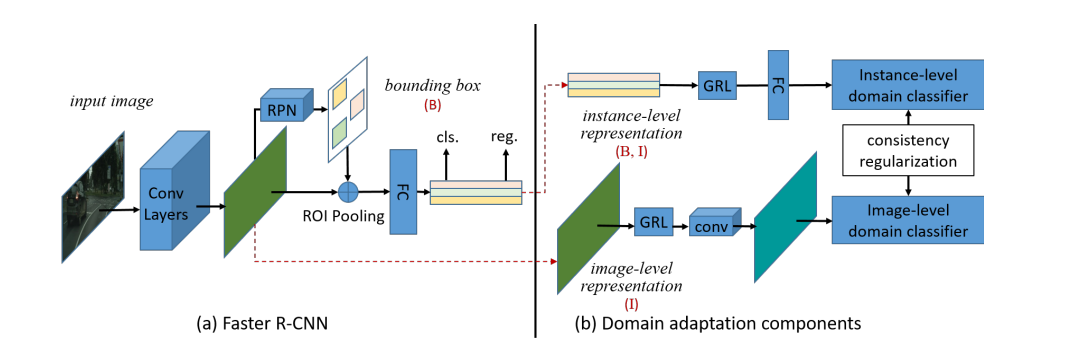
\includegraphics[width=16cm]{./faster_rcnn_DA.png}
	\end{center}
	\caption{Domain Adaptive Faster R-CNN for Object Detection in the Wild \cite{Chen2018}.}
	\begin{center}
		\label{Faster_rcnn_DA}
	\end{center}
\end{figure}

Here, to maximize the domain classification losses $L_{inst}$ and $L_{img}$, they are calculated as shown in Equation \ref{faster_DA_losses}. 

\begin{equation}
\label{faster_DA_losses} 
\begin{gathered}
\mathcal{L}_{i m g}=-\sum_{i, u, v}\left[D_{i} \log p_{i}^{(u, v)}+\left(1-D_{i}\right) \log \left(1-p_{i}^{(u, v)}\right)\right] \\ 
\mathcal{L}_{i n s} = -\sum_{i, j}\left[D_{i} \log p_{i, j}+\left(1-D_{i}\right) \log \left(1-p_{i, j}\right)\right]
\end{gathered}
, 
\end{equation}
where $D_i=0$ is a ground-truth label of the sample image $i$ that originates from  the source domain and $D_i=1$ originates from the target domain; $p_{i,j}$ is a prediction output of the instance-level classifier for $j$-th proposed region of the sample image $i$; $p_{i}^{(u, v)}$ is a prediction output of the image-level domain classifier for the feature map region $(u,v)$ of a sample image $i$ \cite{Chen2018}. 
Finally, two domain classifiers are regularized using consistency loss $\lambda \mathcal{L}_{\text {consistency }}$ \cite{Chen2018} as shown in Equation \ref{faster_DA_losses_consist}.  

\begin{equation}
\label{faster_DA_losses_consist} 
\mathcal{L}_{\text {consistency }}=\sum_{i, j}\left\|\frac{1}{|N|} \sum_{u, v} p_{i}^{(u, v)}-p_{i, j}\right\|_{2}
, 
\end{equation}
Due to the fact that the image-level domain classifier produces multiple $N$ predictions per image, first the average of them is calculated, and then the Euclidean (or L2 norm) distance is measured between the predictions of the image- and instance-level domain classifiers \cite{Chen2018}. 

The final objective of the network is then defined by minimizing the detection loss, while maximizing the image-level $\mathcal{L}_{img}$ and instance-level $\mathcal{L}_{inst}$ domain classification losses. The network additionally aims to minimize the consistency loss $\lambda \mathcal{L}_{\text {consistency }}$ between two classifiers \cite{Chen2018}.

Another most recent state-of-the-art study made by Rezaeianaran et al. \cite{Rezaeianaran2021} proposed different approach that compares the adversarial training to contrastive learning. Similarly to Chen et al. \cite{Chen2018}, the network with adversarial learning leverages a Faster-RCNN detector with instance- and image-level alignments. Rezaeianaran et al. also attempted a different approach for instance-level alignment by pushing the features closer in both domains if they represent the same class, and push them apart otherwise. This is performed by utilizing a max-margin contrastive loss. The margin here denotes how far the features can be in order to be considered to represent the same class. According to Rezaeianaran et al. \cite{Rezaeianaran2021}, a general constrastive loss term takes the form of Equation \ref{contrastiveL}:

\begin{equation}
\mathcal{L}_{C L}=\sum_{i}^{N}\left[\left\|\mathcal{F}_{S}^{i}-\mathcal{F}_{T}^{i}\right\|_{2}^{2}+\sum_{j, j \neq i}^{N} \max \left\{0, m-\left\|\mathcal{F}_{S}^{i}-\mathcal{F}_{T}^{j}\right\|_{2}^{2}\right\}\right],
\label{contrastiveL} 
\end{equation}

where $m$ is the max-margin value and $N$ is the number of classes. 

\begin{figure}[htb]
	\begin{center}
		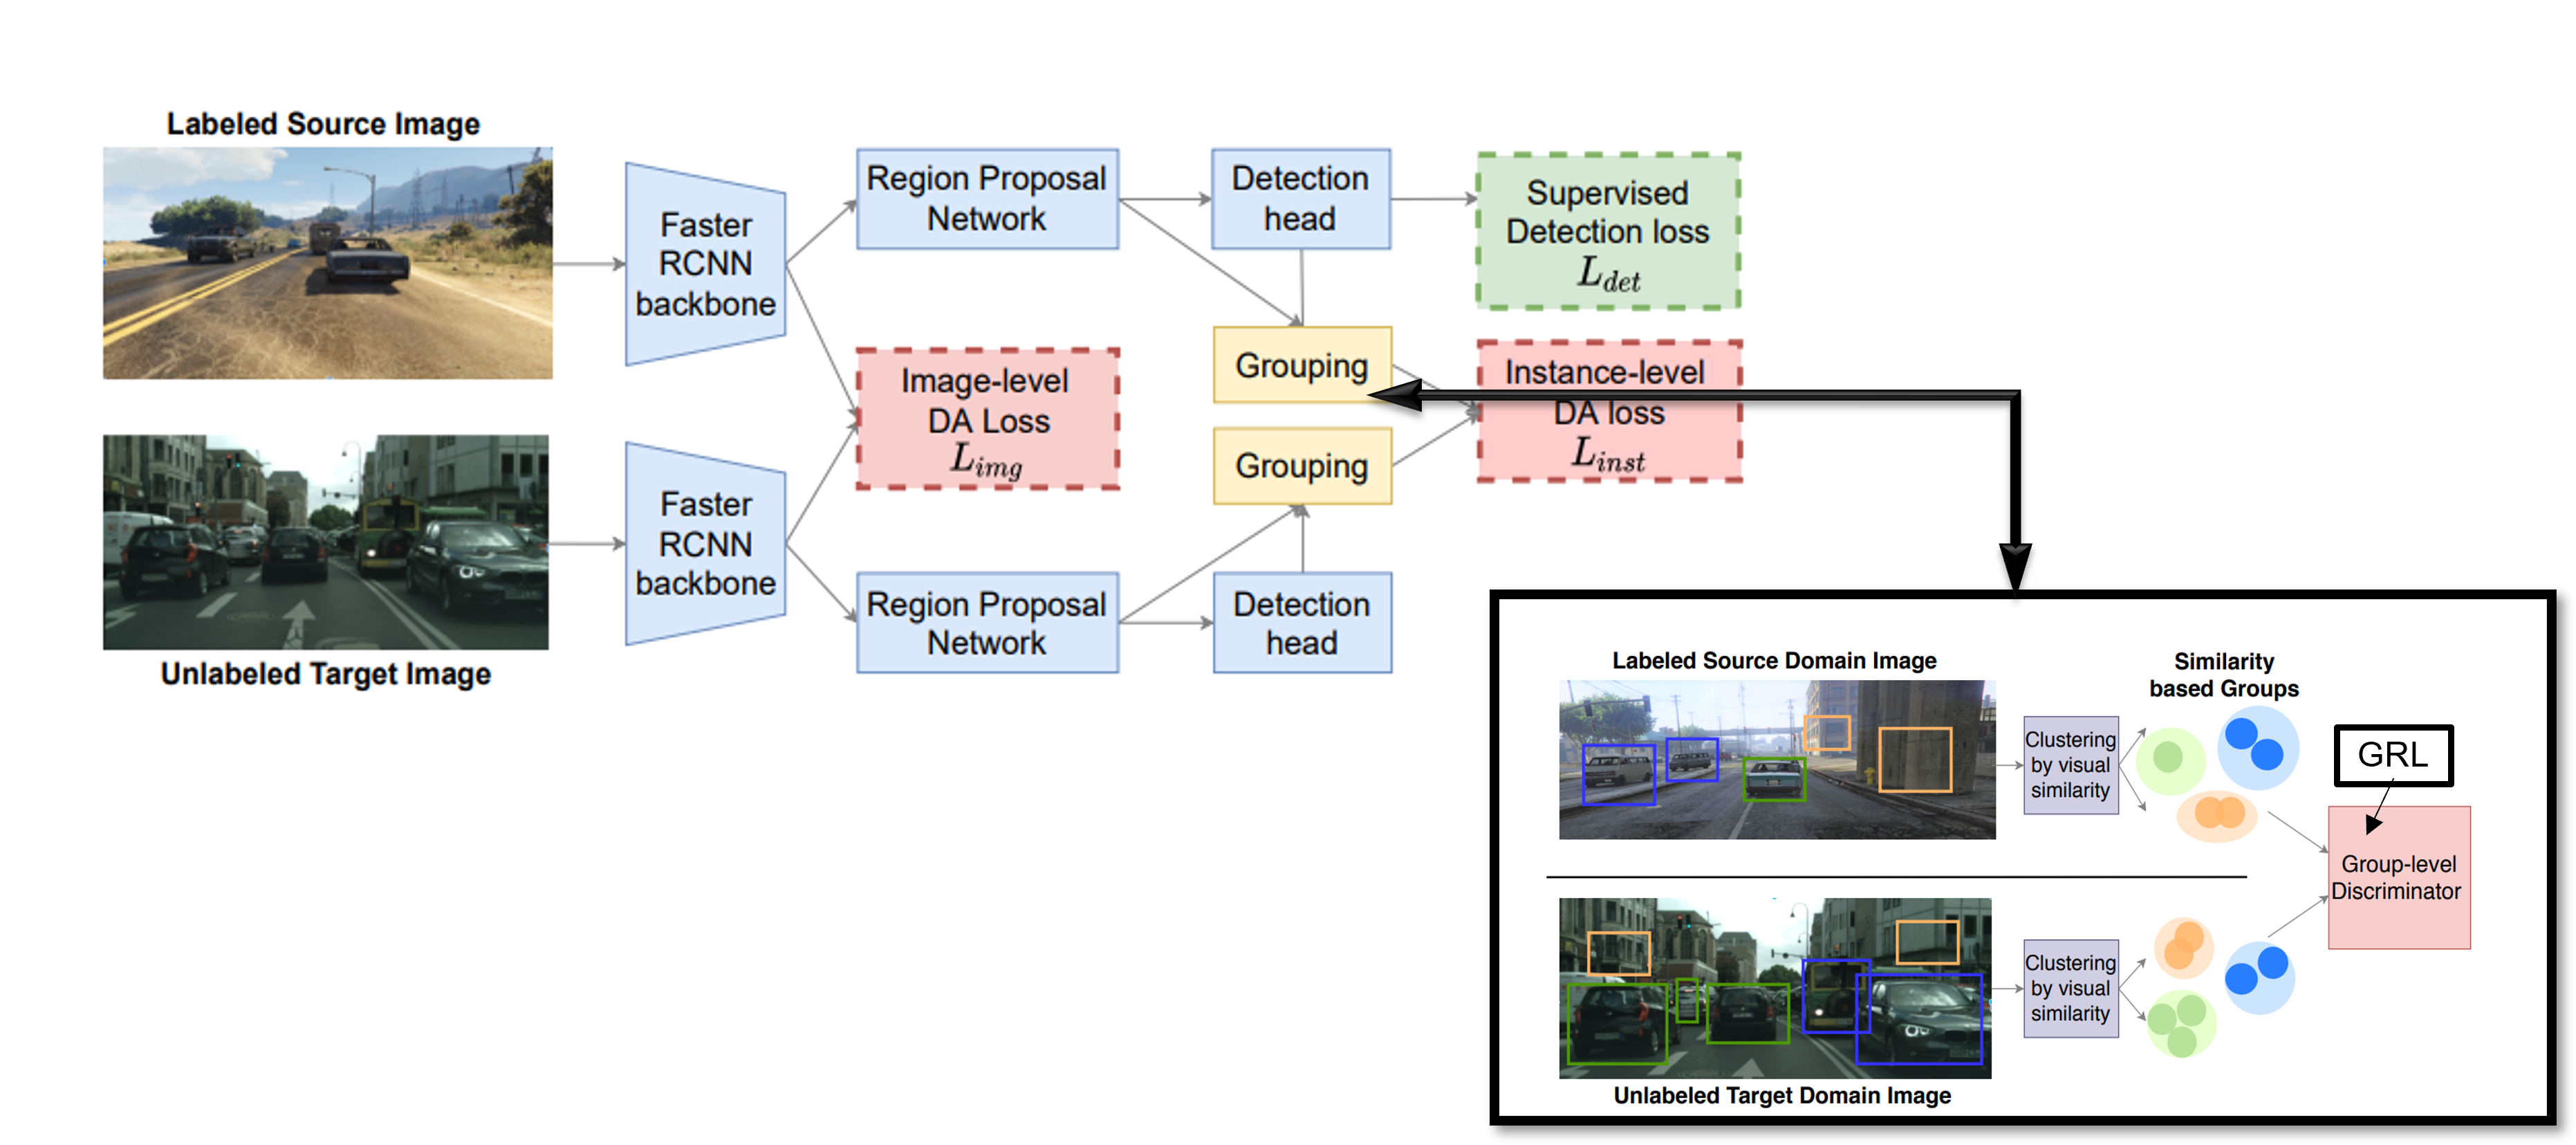
\includegraphics[width=16cm]{./VisGa.png}
	\end{center}
	\caption{Seeking Similarities over Differences: Similarity-based Domain Alignment for Adaptive Object Detection, adapted from \cite{Rezaeianaran2021}.}
	\begin{center}
		\label{visga}
	\end{center}
\end{figure}

Rezaeianaran et al. suggested that using only image-level domain adaptation might force the alignment of the background features relevant to the source domain (images from the simulator). For this reason, the authors proposed to first group the generated features using similarity-based clustering. Initially, all proposed regions are considered to be separate clusters. Next, at every  iteration, two closest clusters are merged based on the cosine distance. After this algorithm has converged, the average of the instances in each cluster is generated. The aggregated average proposal is then processed on a group-level in a standard adversarial manner using a GRL and a domain classifier. 
\FloatBarrier

\subsubsection{Pseudo-labeling based methods}

Another relatively straightforward method to solve an object detection problem can be done by using pseudo-labels. A naive approach to pseudo-labeling is to first train the source dataset $\mathcal{D}_{\mathcal{S}}=\left\{\mathcal{X}_{\mathcal{S}}^{i}, \mathcal{Y}_{\mathcal{S}}^{i}\right\}_{i=1}^{\mathcal{N}_{\mathcal{S}}}$ and later run inference to obtain pseudo-labels on the target dataset $\mathcal{D}_{\mathcal{T}}=\left\{\mathcal{X}_{\mathcal{T}}^{j}\right\}_{j=1}^{\mathcal{N}_{\mathcal{T}}}$. The resulted labels will then form a new dataset $\dot{\mathcal{D}_{\mathcal{T}}}=\left\{\mathcal{X}_{\mathcal{T}}^{j}, \mathcal{Y}_{\mathcal{T}}^{j}\right\}_{j=1}^{\mathcal{N}_{\mathcal{T}}}$ \cite{Oza2021}. However, the results obtained will naturally be noisy and of poor quality. Khodabandeh et al. proposed a three-phase training process illustrated in Figure \ref{robust} below. 

\begin{figure}[htb]
	\begin{center}
		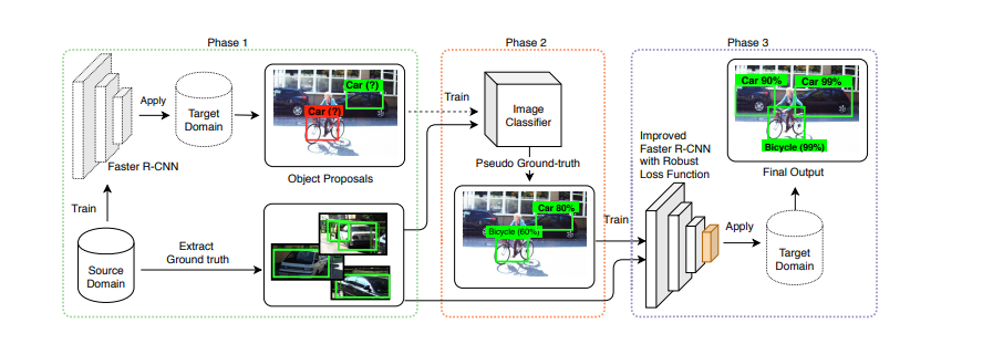
\includegraphics[width=16cm]{./robust.png}
	\end{center}
	\caption{A Robust Learning Approach to Domain Adaptive Object Detection \cite{Khodabandeh2019}.}
	\begin{center}
		\label{robust}
	\end{center}
\end{figure}

In the first stage, the network is treated as a typical Faster-RCNN network that is trained on the source dataset $\mathcal{D_S}$. Next, the pseudo-labels are generated as explained earlier. In the following stage, the proposed regions are fed into a pre-trained image classifier, which allows to refine the model.

For the process of refinement, Khodabandeh et al. proposed to use the Kullback-Leibler divergence and defined the optimization objective for classification as follows: 

\begin{equation}
\min _{q} \operatorname{KL}\left(q\left(y_{c}\right) \| p_{c l s}\left(y_{c} \mid \boldsymbol{x}, \tilde{\boldsymbol{y}}_{l}\right)\right)+\alpha \operatorname{KL}\left(q\left(y_{c}\right)|| p_{i m g}\left(y_{c} \mid \boldsymbol{x}, \tilde{\boldsymbol{y}}_{l}\right)\right)
\label{KL_DV} 
,
\end{equation}

where $y_c$ is the class label, $y_l$ is the bounding box location, $\alpha$ is a trade-off between two terms,  $p_{img}$ is the classification prediction of the image classification model and $p_{cls}$ is the classification prediction of the Faster-RCNN detector model \cite{Khodabandeh2019}. The goal of the refining process is to find a distribution $q(y_c)$ that is close to the models of $p_{cls}$ and $p_{img}$. The process is relatively similar for the bounding box refinement and the reader is advised to consult the original paper for more details \cite{Khodabandeh2019}.  

The third stage of the process finalizes the strategy by retraining the final network with the labeled ground truth data from $\mathcal{D_S}$ and the refined pseudo-labels from $\dot{\mathcal{D_T}}$. 
\FloatBarrier


\subsubsection{Image-to-Image translation}
\label{imagetoimage} 
Another category that Oza et al. \cite{Oza2021} outlined is image-to-image translation for UDA. Instead of trying to align features, this group of methods essentially attempt to pull the domains together first. Hsu et al. \cite{Hsu2019} has suggested a Cycle-Generative Adversarial Network(GAN) \cite{Zhu2017} based approach to transform images from the target domain into the source domain alike images. Figure \ref{gan} represents the complete network proposed by Hsu et al. 

\begin{figure}[htb]
	\begin{center}
		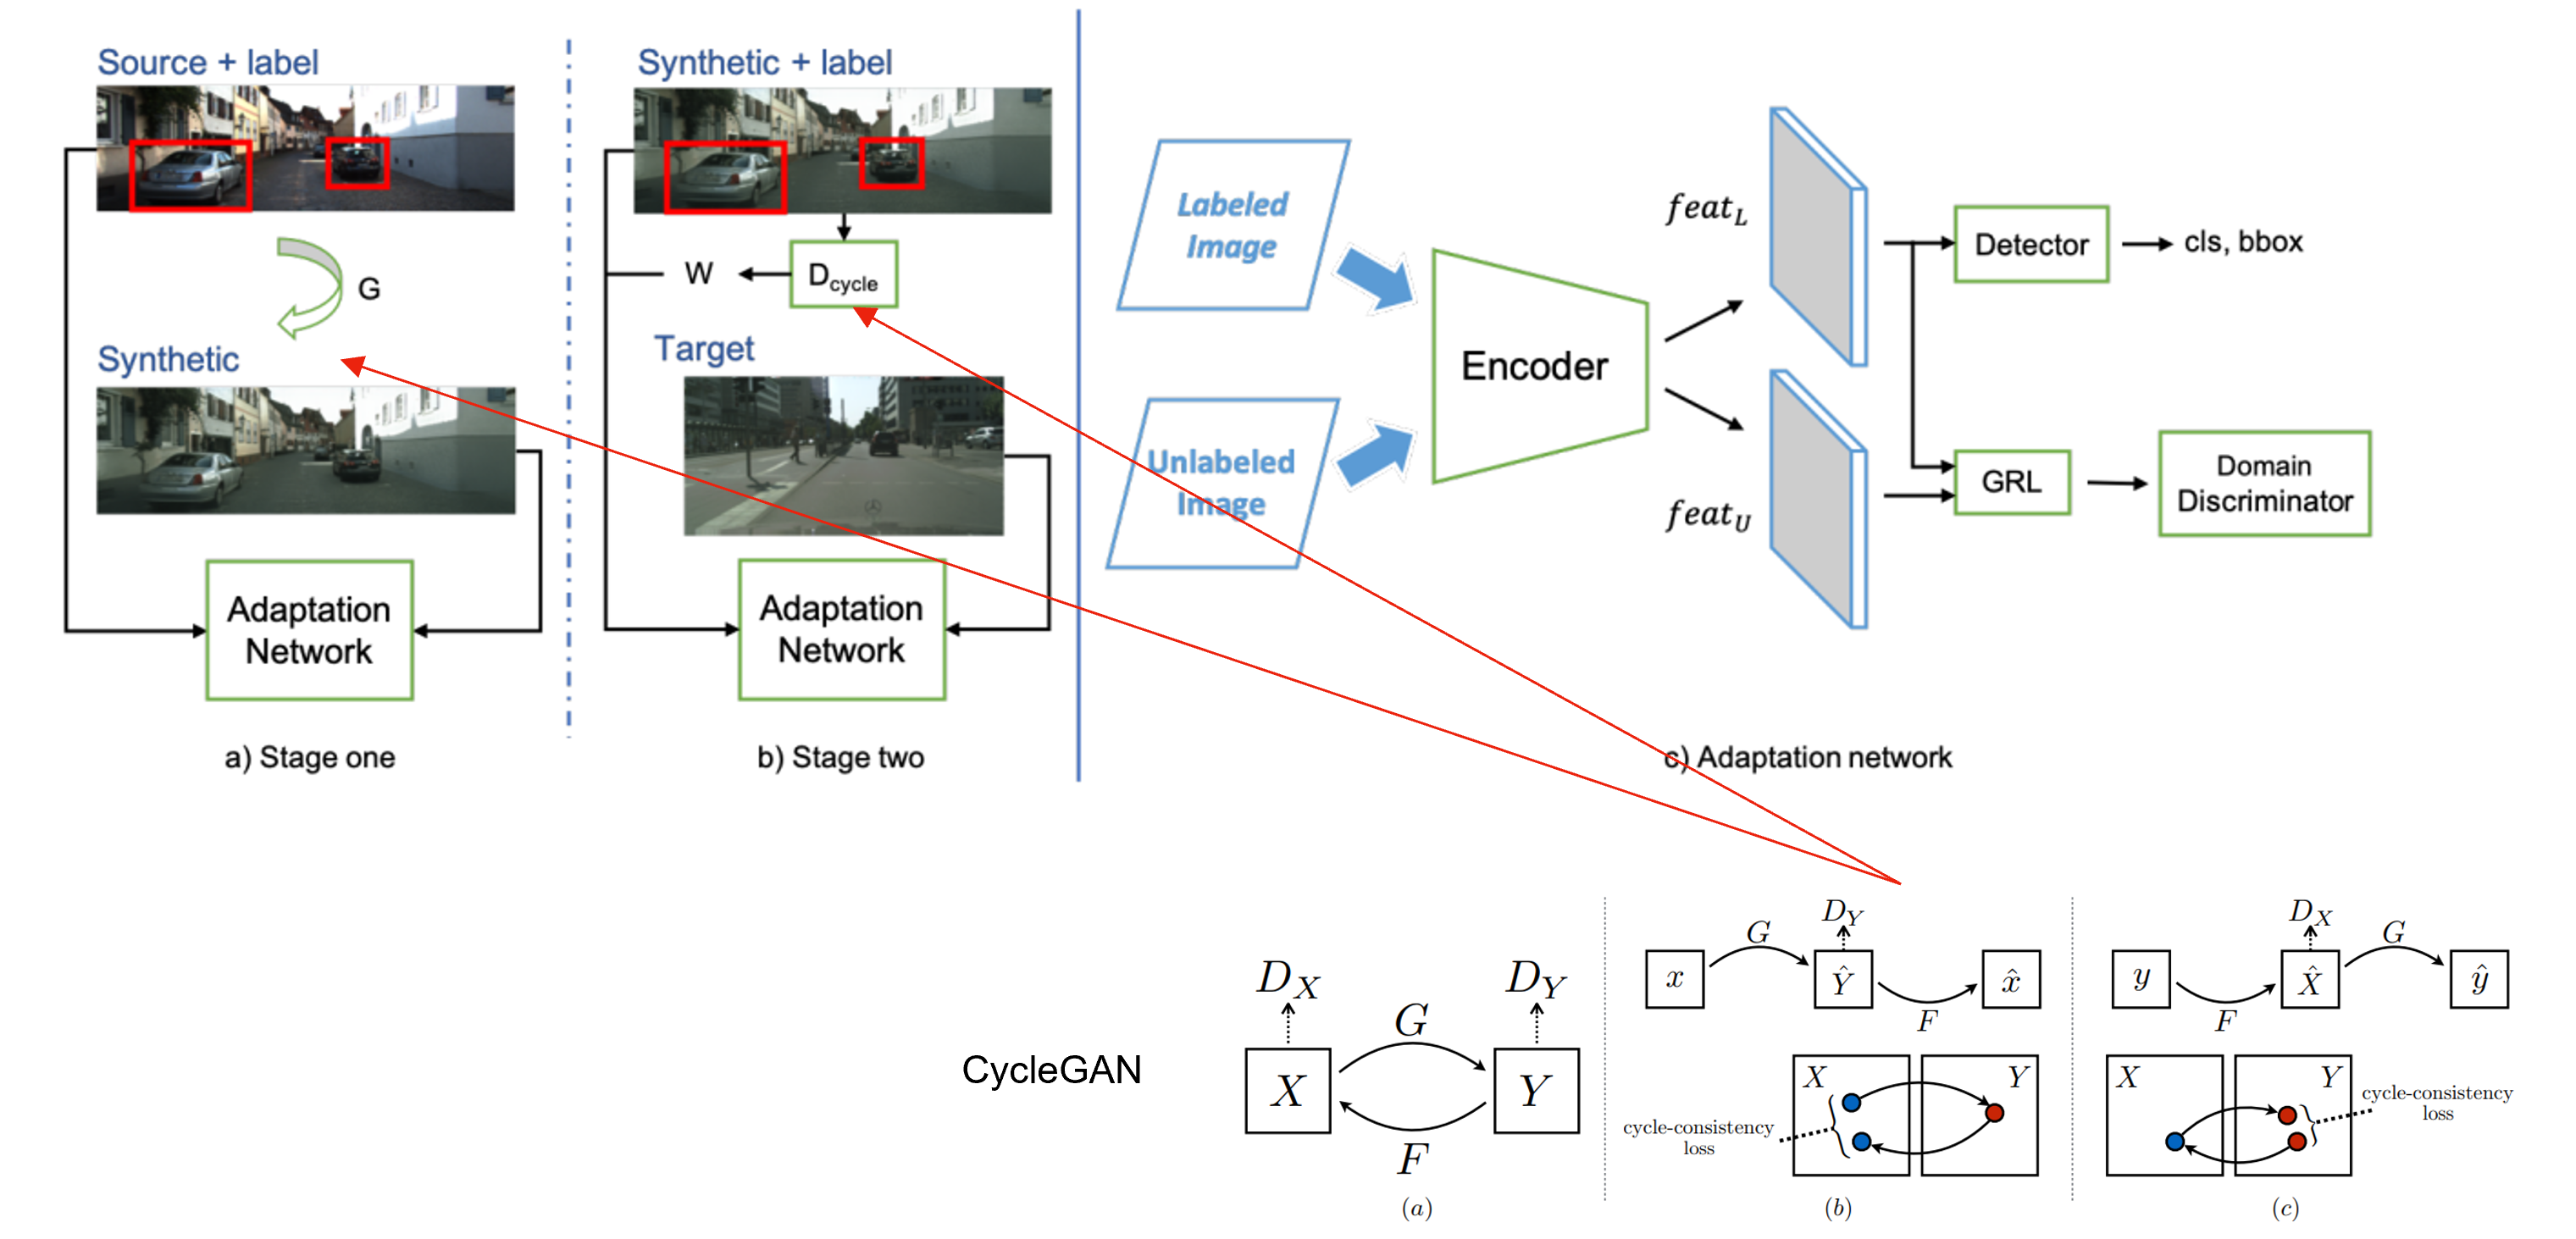
\includegraphics[width=16cm]{./GAN.png}
	\end{center}
	\caption{Progressive Domain Adaptation for Object Detection and CycleGAN, adapted from \cite{Hsu2019}.}
	\begin{center}
		\label{gan}
	\end{center}
\end{figure}

The generator part of the Cycle-GAN in Figure \ref{gan} (a) creates intermediate domain from images in the source domain. The source images are then passed together with the labels to the Faster-RCNN network. The network is then tries to adapt the source domain to the synthetic domain. To further minimize the domain shift, adversarial learning techniques are used, such as a combination of a GRL and a domain classifier \cite{Hsu2019}.


In Figure \ref{gan} (b), the synthetic source-alike images are then passed together with the inherited source labels back to the adaptation network to align the features with the target domain. In the second stage of the training process, Hsu et al. proposed to utilize the weights $w$ from the discriminator of the Cycle-GAN, which is additionally trained to differentiate between source and target domains. Ultimately, such approach allowed to amplify the importance of the synthetic samples that are closer to the target domain. The weighted loss from the discriminator was then summed with the detection loss and the adversarial loss to finally adapt the synthetic domain to target \cite{Hsu2019}. 
\FloatBarrier

\subsubsection{Domain randomization}

Oza et al. \cite{Oza2021} argues that often the accuracy of image-to-image translation methods is questionable as the domain shift between the synthetic and source domains still exists. Slightly different approach has been offered by Kim et al. \cite{Kim2019}. Instead of trying to pull two given domain distributions closer, they proposed a domain randomization technique, which generally attempts to generate a brand new domain that includes the same image in different style. This in practice allows the detector network to recognize features that are domain invariant and remove the domain bias. 

Kim et al. proposed a detector network that is based on Faster-RCNN with two additional components. The first component is a domain diversification module. Similarly to the method proposed by Hsu et al. \cite{Hsu2019}, the module leverages a Cycle-GAN \cite{Zhu2017}. However, the diversification module is used to generate images in a fixed set of new domains rather than to match the source dataset with target.  The second component is a multi-domain discriminator, which is essentially an adversarial feature learning approach, but instead of trying to confuse the detector in a binary set of domains, it tries to learn domain invariant features of multiple additional domains. The architecture of such domain randomization method is presented in Figure \ref{diversify}.

\begin{figure}[htb]
	\begin{center}
		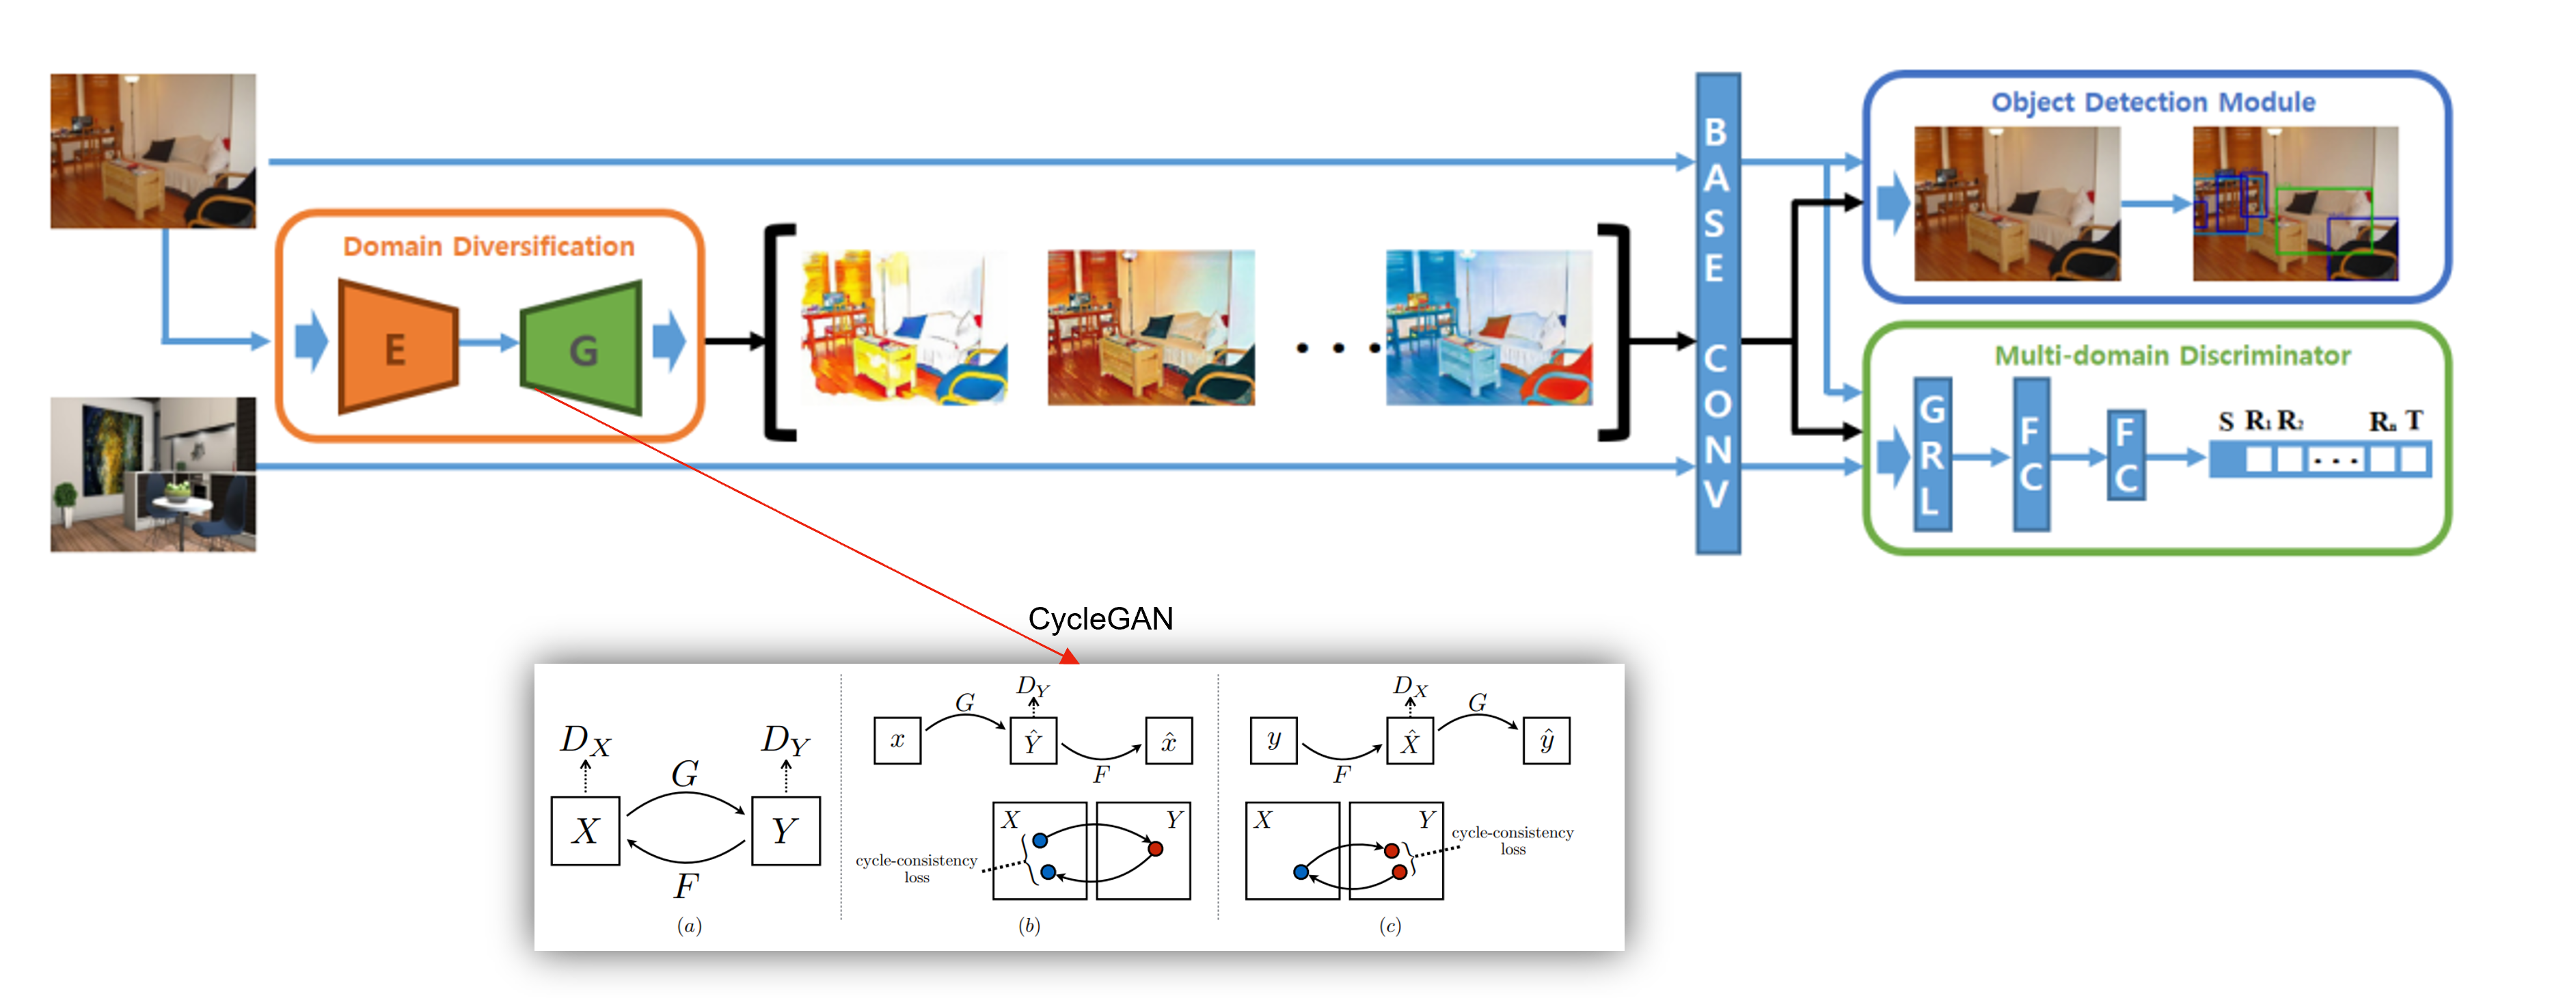
\includegraphics[width=16cm]{./diversify.png}
	\end{center}
	\caption{Diversify and Match: A Domain Adaptive Representation Learning Paradigm for Object Detection, adapted from \cite{Kim2019}.}
	\begin{center}
		\label{diversify}
	\end{center}
\end{figure}

During Cycle-GAN image generation, two additional loss terms limited the  randomization of an image - color preservation and reconstruction constraints. This was done in order to preserve features of the original image as it would otherwise affect the model negatively \cite{Oza2021}. In the original experiments Kim et al. considered three additional domains: a color preserved domain, a reconstructed domain, and a domain that combines both. Images from all the domains are then fed into the detector along with the inherited source labels   to train a domain-invariant network with help of a multi-class domain classifier and the resulted model was used to verify performance on the target dataset. 
\FloatBarrier

\subsubsection{Mean Teacher and Graph Reasoning}
\label{mean_teacher} 
Another common approach utilized in domain adaptation and transfer learning in general is mean teacher training. A typical mean teacher setup consists of two equivalent models. However, these models are trained using two separate strategies to adapt the detector network. On the other hand, graph reasoning based approaches of UDA have been gaining popularity not only in image classification problems, but also in object detectors. One potential reason for this is because graph models are easily applicable with other adaptation methodologies \cite{Oza2021}. Cai et al. \cite{Cai2019} proposed an architecture that combines both mean teacher and graph reasoning techniques in one solution and such architecture is presented in Figure \ref{graph_MT}. 
 
\begin{figure}[htb]
	\begin{center}
		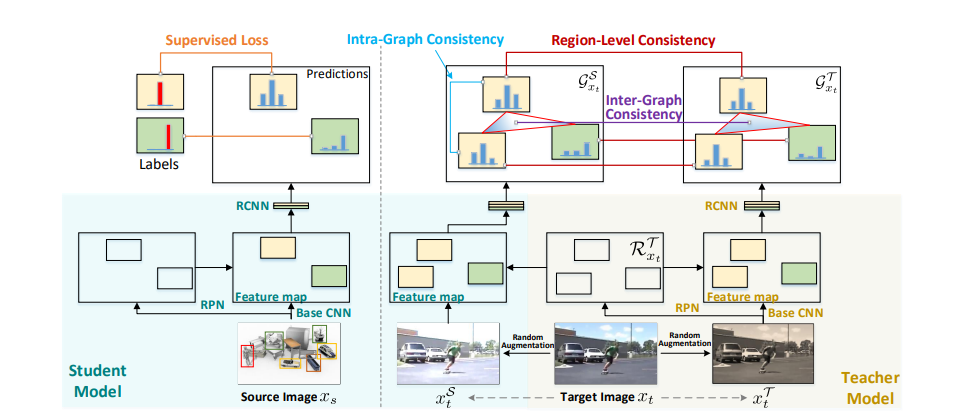
\includegraphics[width=16cm]{./graph_teacher.png}
	\end{center}
	\caption{Exploring Object Relation in Mean Teacher for Cross-Domain Detection \cite{Cai2019}.}
	\begin{center}
		\label{graph_MT}
	\end{center}
\end{figure}

The term "graphs" represents a complex data structure that contains multiple nodes or vertices connected to each other via edges. In case of an image as a graph, each pixel can be considered a node, which is linked to all of its neighbors. 
The setup developed by Cai et al. \cite{Cai2019} introduces a student-teacher framework based on Faster-RCNN that verifies the consistency of the graphs at three different levels using regional-level consistency, intra-graph consistency and inter-graph consistency. 

The training pipeline is split into two parts. Images from the source domain are trained in a locked student environment in a supervised manner.  On the other hand, images from the target domain are augmented in two steps. First, the images are randomly cropped, padded or flipped. These images are passed through the pre-trained supervised student model that generates predictions. Meanwhile, the original target images are augmented with color jittering or corruption with noise. This set is send to the teacher model. The teacher model also produces predictions, which are then compared with the predictions from the first set of augmented images by utilizing region-level consistency. Essentially, the region-level consistency is calculated as MSE of the region-level prediction error in  both the student and the teacher. 

Inter-graph level consistency is used to verify the quality of the two graphs produced by the teacher and student models. It is calculated by means of cosine similarity between the graph representations of the proposed regions. 

Finally, intra-level consistency is then calculated to measure the quality of predictions within the same class of the student model. However, since target domain has no labels included in the UDA setup, the closest prediction $\operatorname{argmin} (labels)$ is used to produce pseudo-labels. The intra-level consistency loss is then calculated for any two instances of the same class in one graph. For more detailed calculation of the loss terms the readers are referred to the original paper by Cai et al. \cite{Cai2019}.

A purely mean-teacher-based semi-supervised approach has been proposed by Liu et al. \cite{Liu2021} As it can be seen from the overview illustrated in Figure \ref{unbiased}, it consists of two sequential stages. During the burn-in stage, Faster-RCNN detector is trained on the labeled data as normal. Next, the training pipeline is split into two equivalent Faster-RCNN-based detectors. The teacher model is supplied with weakly-augmented data. On the other hand, strongly-augmented images are fed into the student model. According to Liu et al., the main reason for that was because while strong augmentation is needed to improve performance of the model, the weaker augmentations were still needed in the teacher model to generate reliable pseudo-labels. These pseudo-labels are in turn used in the student model.   
\begin{figure}[htb]
	\begin{center}
		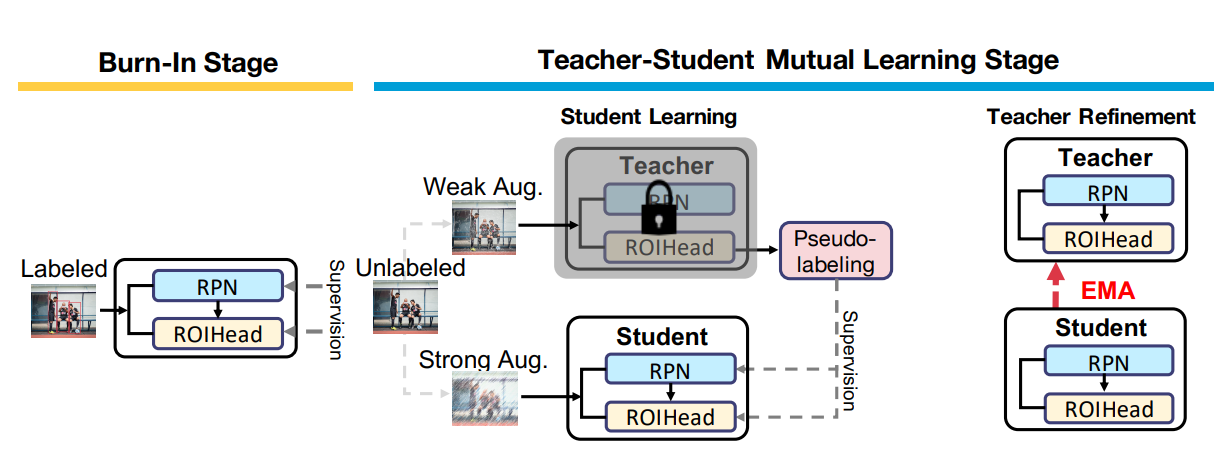
\includegraphics[width=14cm]{./unbiased.png}
	\end{center}
	\caption{Unbiased Teacher for Semi-Supervised Object Detection \cite{Liu2021}.}\label{unbiased}
	\begin{center}
	\end{center}
\end{figure}

In order to achieve higher accuracy of pseudo-labels, the unbiased teacher model includes an Exponential Moving Average(EMA) module, along with a few other techniques \cite{Liu2021}. EMA attempts to emphasize the most recent data by granting it a higher weight. The EMA in Unbiased teacher is defined as follows: 
\begin{equation}
\theta_{t}^{i}=\hat{\theta}-\gamma \sum_{j=1}^{i-1}\left(1-\alpha^{-j+(i-1)}\right) \frac{\partial\left(\mathcal{L}_{\text {sup }}+\boldsymbol{\lambda}_{u} \mathcal{L}_{u n s u p}\right)}{\partial \theta_{s}^{j}}
\label{EMA}
,
\end{equation}

where $\hat{\theta}$ is the initial (burn-in stage) model weight, $\theta_{t}^{i}$ is the weight of the teacher model, $\theta_{s}^{j}$ is the weight of the student model  at $i$-th and $j$-th iterations respectively. The weight of EMA in the training process is defined by $\alpha$ and $\gamma$ is the learning rate(LR) of the ensembled model \cite{Liu2021}.

Liu et al. also discusses the class imbalance problem that often causes the detector to learn underrepresented classes poorly \cite{Liu2021}. In order to solve this problem, Liu et al. propose to make use of the multi-focal loss \cite{Lin2017}, which attempts to put more weight on the samples with lower confidence, unlike a generic cross-entropy loss that treats all samples equally. 

However, this method only solves a semi-supervised object detection without addressing the domain shift issue. Expanding the unbiased teacher method, Li et al. \cite{Li2021} proposed to utilize mean teacher training in a domain adaptation setup. In addition to the original ensembled network proposed by Liu et al.  \cite{Liu2021}, Adaptive Teacher architecture employs adversarial feature learning techniques to adapt the target domain to the source. A typical domain adaptation network, which includes a GRL and a domain classifier, is appended to the backbone feature extractor of the student model. The complete architecture is displayed in Figure \ref{adapt_teacher}. 
 
\begin{figure}[htb]
	\begin{center}
		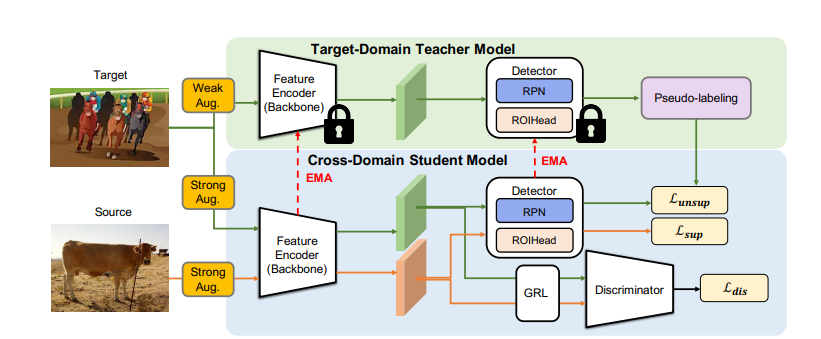
\includegraphics[width=16cm]{./adapt_teacher.png}
	\end{center}
	\caption{Cross-Domain Adaptive Teacher for Object Detection
\cite{Li2021}.}
	\begin{center}
		\label{adapt_teacher}
	\end{center}
\end{figure}

Liu et al. \cite{Liu2021} specified that the teacher model is supplied with weakly-augmented target images, while the student model uses both strongly-augmented source and target images. Weak augmentations include cropping and flipping the image horizontally, and strong augmentations included grayscaling, color jittering, Gaussian blurring and cutting out patches. The same strategy was employed in this Adaptive Teacher method. The augmentations used in these works  \cite{Li2021, Liu2021} are presented in Figure \ref{augmentations}. 
\begin{figure}[htb]
	\begin{center}
		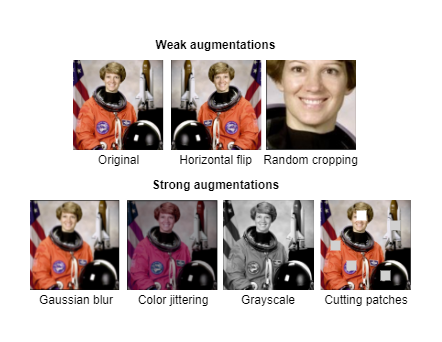
\includegraphics[width=10cm]{./augmentations.png}
	\end{center}
	\caption{Augmentations used in Unbiased teacher (adapted from the official Pytorch documentation \cite{pytorch}).}
	\begin{center}
		\label{augmentations}
	\end{center}
\end{figure}


Although all of the methods discussed in this chapter are based on the two-stage object detector Faster-RCNN, fewer papers also addressed a single-stage object detection in a domain adaptation setup, such as UDA for YOLO \cite{Hnewa2021}, \cite{Zhang2021a}, UDA for FCOS \cite{fcos1} and UDA for DETR \cite{Zhang2021b}, \cite{Vidit2021}. However, their review will be omitted with the grounds for it given in the \nameref{Methodology} section. 
\FloatBarrier

\subsection{Continual learning}
\label{cont_learning} 
While traditional transfer learning attempts to apply knowledge collected from one domain to another, lifelong learning offers adaptive algorithms, which  would accept a continuous stream of information that becomes available over time \cite{Parisi2018}. In case of the simple object detection problem, continual learning can be applied to a new task, such as to learn new classes of objects that are supplied progressively over time. This approach is potentially useful due to the scalability benefits it brings, since retraining the entire model every time a new object arrives to the database is computationally expensive. 

Similarly to the human brain, ANNs in object detectors tend to forget old knowledge learned as the memory gets overwritten with fresh data. This phenomenon in continual learning is commonly addressed as "catastrophic forgetting" \cite{Parisi2018}. Parisi et al. summarizes the up-to-date methods of continual learning that are effective against catastrophic forgetting into three categories: retraining with regularization, selective training with network expansion and retraining selective network with expansion. These methods are illustrated in Figure \ref{continual}. 

\begin{figure}[htb]
	\begin{center}
		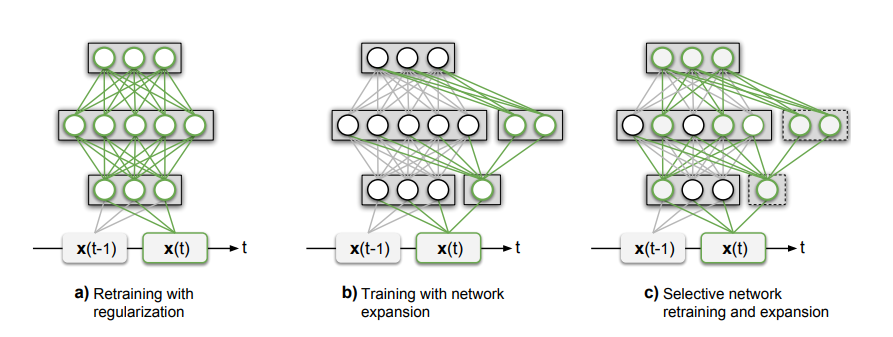
\includegraphics[width=16cm]{./continual.png}
	\end{center}
	\caption{Continual learning approaches
\cite{Parisi2018}.}
	\begin{center}
		\label{continual}
	\end{center}
\end{figure}

The methods proposed in Figure \ref{continual} (a) attempt to solve catastrophic forgetting by means of regularization. In these group of methods, the algorithm seeks to penalize the modifications in the model of the originally trained task. A simplistic approach of such method was presented by Razavian et al.  \cite{Razavian2014}, where the gradients calculation for the parameters of the original is disabled completely. Slightly modified version of this method was also proposed by Donahue et al. \cite{Donahue2013}, where the LR was decreased to minimize the parameter update instead of blocking the update altogether. 


In simplistic terms, the method of training with expansion denotes retraning the original network with an additional number of layers appended. A typical example of such a method was proposed by Rusu et al. \cite{Rusu2016}, where the network was trained on the initial task. As $N$ new tasks were added, $N$ number of layers were appended to the network, as shown in Figure \ref{continual} (b). The parameters of the original network were left unchanged, and only the additional connections were trained. Although the disadvantage of this method was that the network complexity would grow linearly over time as new tasks are added, the experiments delivered sufficient performance. 

The method proposed by Yoon et al. \cite{Yoon2017} falls into the third category, which is illustrated in Figure \ref{continual} (c). The concept is fundamentally similar to the one suggested by Rusu et al. \cite{Rusu2016}, with the exception that their model selectively retrains the network from the original task. Connecting the neurons sparsely reduced the computational overhead, as well as allowed the network to retain the previously learned tasks. Parisi et al. \cite{Parisi2018} have collected many other promising continual learning methods and the reader is advised to refer to the original survey for more details.   

In the context of the notation defined earlier in the \nameref{transferLearning} subsection, continual learning can be expressed as training on the task $\mathcal{T}_n$ given the task $\mathcal{T}_{n-1}$ within the same domain or a set of domains $\mathcal{D}_{n} = \mathcal{D}_{n-1}$.   

\FloatBarrier

\clearpage  
\section{Research Methodology}
\label{Methodology}

In this section, an in-depth study will be conducted to solve the challenges outlined in the \nameref{objective}. The section will first discuss the process of dataset selection. Next, several object detection candidates will be analyzed.  The selected object detection method will be examined in multiple domain-adaptive setups. Upon analyzing the existing DA methods, one candidate will be studied in greater detail to propose a novel architecture. Finally, continual learning will be investigated in the selected cross-domain object detection model. 


\subsection{Dataset}
\label{datasets} 
One of the objectives of this thesis was to implement an identification system using images of the equipment and images of the 3D models to expand the dataset. 3D images of the equipment can potentially be the main source of the dataset. Autodesk Navisworks offers a possibility of rendering both images and videos of the desired equipment. In order to make the process of data collection scalable, it was proposed to use Navisworks API to automate the process. Following the documentation of the API  \cite{navisworks}, a simple script with an extra toolbox was used to filter out the required model from Navisworks, to render and to export images in \texttt{.jpg} format. The results are presented in Figure \ref{navisworks} below.

\begin{figure}[htb]
    \centering
    \subfloat{{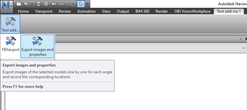
\includegraphics[width=6cm]{./toolbox.png} }}%
    \qquad
    \subfloat{{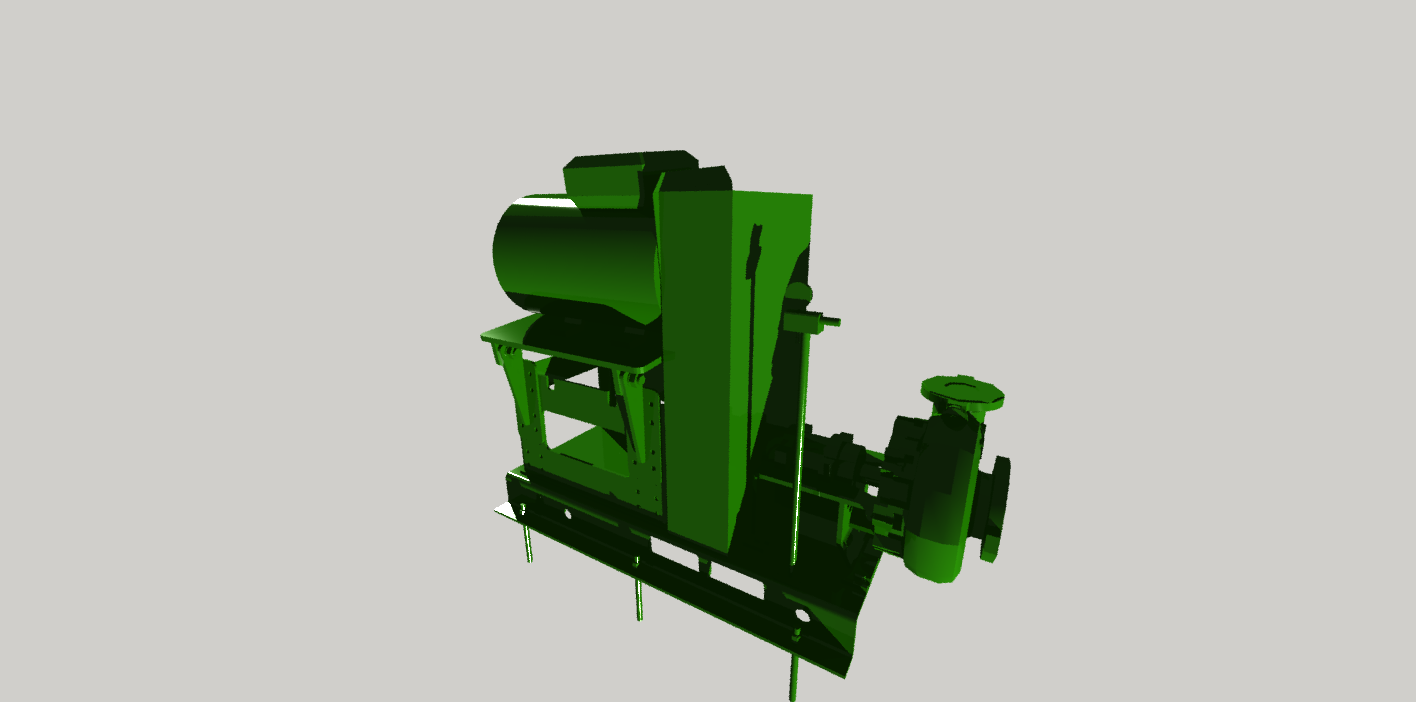
\includegraphics[width=6cm]{./model.png} }}%
    \caption{Example of the rendered image of an arbitrary model}\label{navisworks}%
\end{figure}
\FloatBarrier

It is possible to automatically rotate around the selected object in order to render images from all sides of the equipment as it is important to have variety while accumulating a dataset. However, due to the time constraints, it was decided to leverage existing open-source datasets for the purpose of this study. 

Previously, in the \nameref{neural_nets} section, few datasets, such as ImageNet \cite{Russakovsky2014}, PASCAL VOC \cite{Everingham10} and COCO \cite{Lin2014} were briefly mentioned. These datasets are universally used in image classification and object detection problems. However, in order to leave room for further research as well as to align with the objectives of the thesis, the dataset should ideally consist of industrial equipment and include corresponding 3D models for each object. Datasets such as ImageNet, PASCAL VOC and COCO typically contain generic objects that people face in everyday life. 

Ultimately, it was concluded that the dataset named Texture-LESS(T-LESS)  \cite{hodan2017tless} meets the requirements. It consists of nearly 39 000 training and 10 000 testing images of thirty industry-relevant objects. The training subset consists of rendered images in a simulated environment, while the test subset is taken in real-life conditions.  Different objects in the dataset are often distantly similar to each other, which makes the task slightly more challenging. Finally, the dataset also includes Computer-Aided-Design(CAD) \texttt{.ply} files with 3D models of the objects, which can then be easily converted into any other required CAD format. The dataset is originally meant for 6D-pose estimation \cite{hodan2017tless} as a part of the Benchmark for Pose Estimation(BOP) challenge \cite{hodan2018bop}. As a result, the format of the dataset is derived from the format defined by BOP \cite{hodan2018bop_format}. A script was developed to convert it into a format commonly used by the state-of-the-art object detection frameworks, as well as to remove redundant information that is only applicable to pose estimation tasks. Initially, the dataset was converted to mimic YOLO \cite{Redmon2015a} format, but later it was switched to PASCAL VOC due to its better flexibility in two-stage object detectors. An example of the annotated T-LESS image from a real setup is illustrated in Figure \ref{tless_real_example}. 

\begin{figure}[htb]
	\begin{center}
		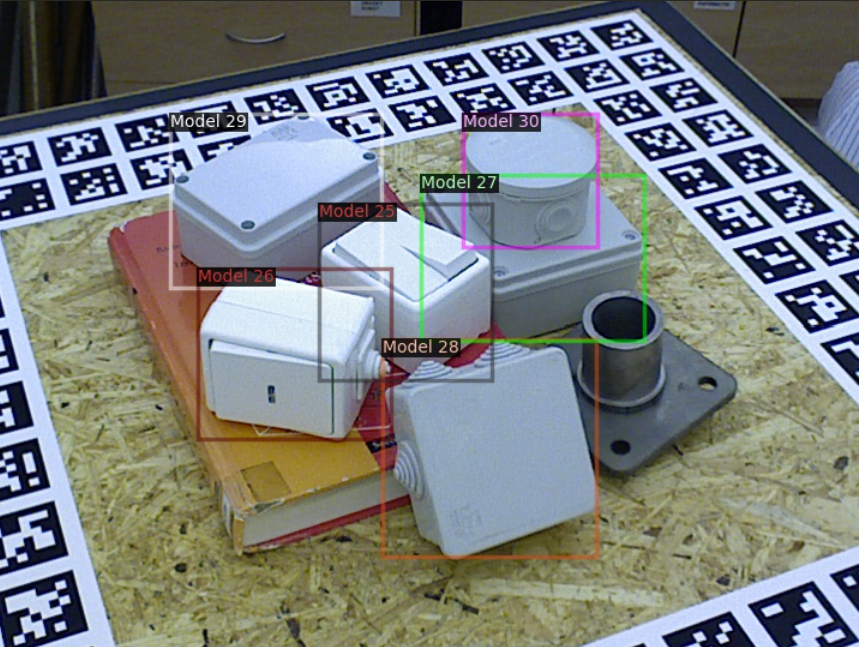
\includegraphics[width=10cm]{./tless_real_annotated.png}
	\end{center}
	\caption{T-LESS real setup, labeled
\cite{hodan2017tless}.}
	\begin{center}
		\label{tless_real_example}
	\end{center}
\end{figure}
\FloatBarrier

The names of the object classes presented in T-LESS, although undisclosed, are irrelevant to this thesis. Therefore, here and in the subsequent sections, when referred to individually, the classes will be named as "Model $N$". Additionally, in the experiments, the datasets with images from the simulator and the images from the real environment setup will be mainly referred to as "source" and "target" datasets, respectively. The images from the source dataset are saved in \texttt{.jpg} format, while the real images are stored as \texttt{.png} files, similarly as in the original T-LESS \cite{hodan2017tless}. Furthermore, for this work, the source dataset will be split in 85\%/15\%  proportion into the training and testing subsets. The distribution of the classes in the source dataset is presented in Figure \ref{tless_distribution_rend}.  

\begin{figure}[htb]
	\begin{center}
		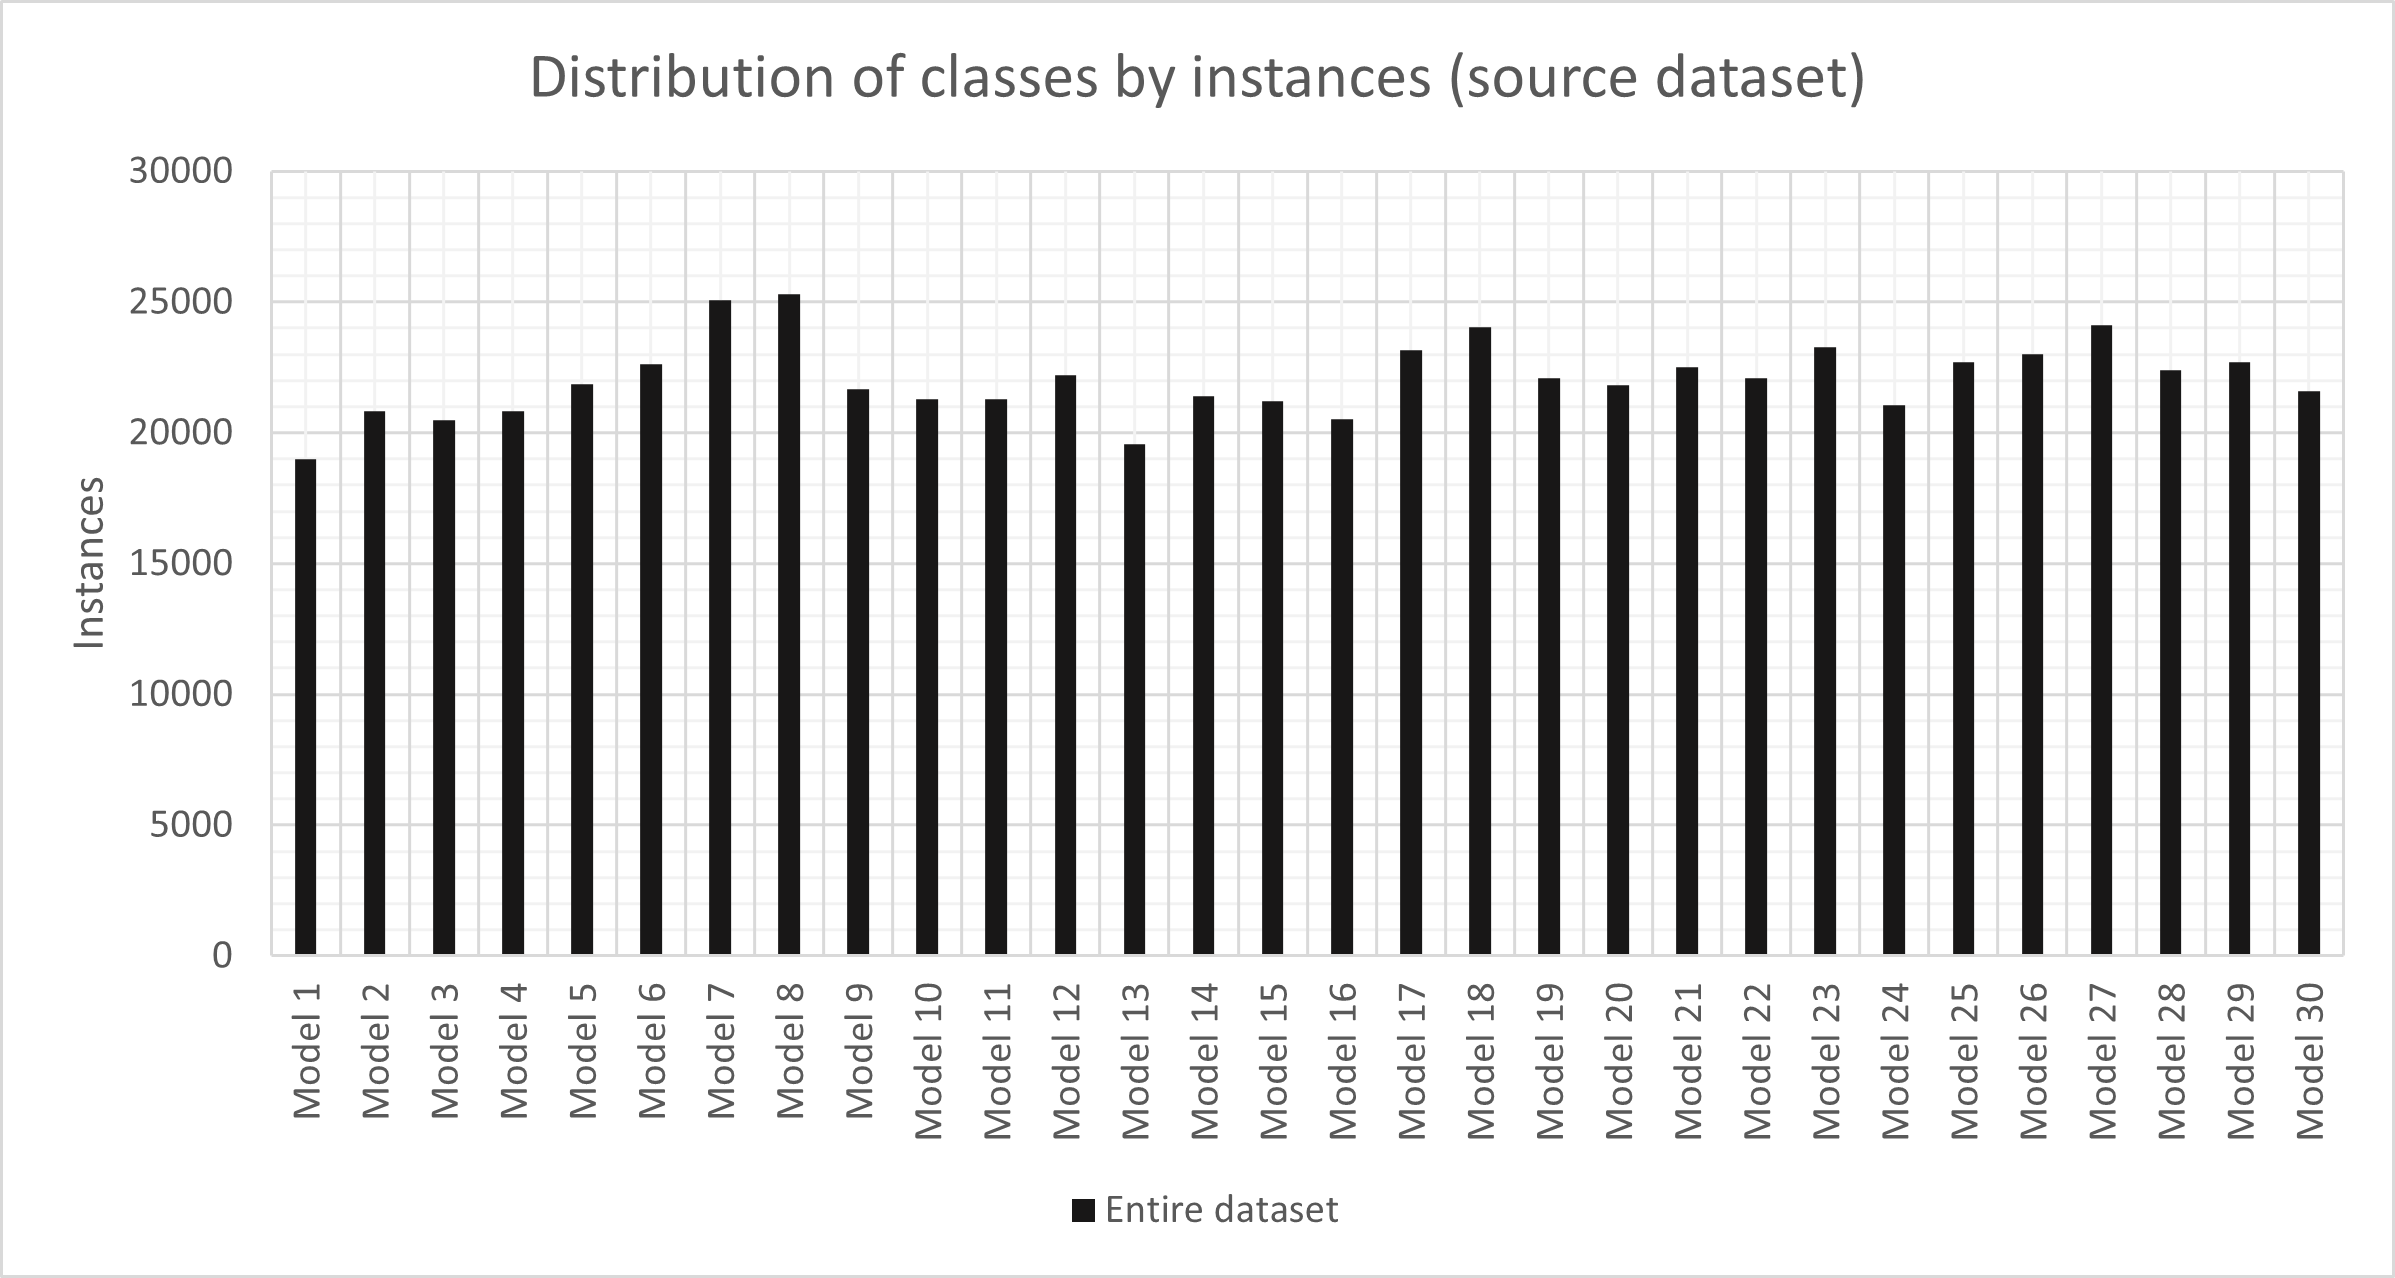
\includegraphics[width=14cm]{./rendered_distribution.png}
	\end{center}
	\caption{Distribution of the classes in the rendered subset of T-LESS dataset. 42 500 and 7 500 training and testing images, respectively. Total number of object instances: 720443}
	\begin{center}
		\label{tless_distribution_rend}
	\end{center}
\end{figure}
\FloatBarrier

On the countrary, real images are only used for validation and their distribution by class is shown in Figure \ref{tless_distribution_real}. The reasons for this will be discussed in later sections. 

\begin{figure}[htb]
	\begin{center}
		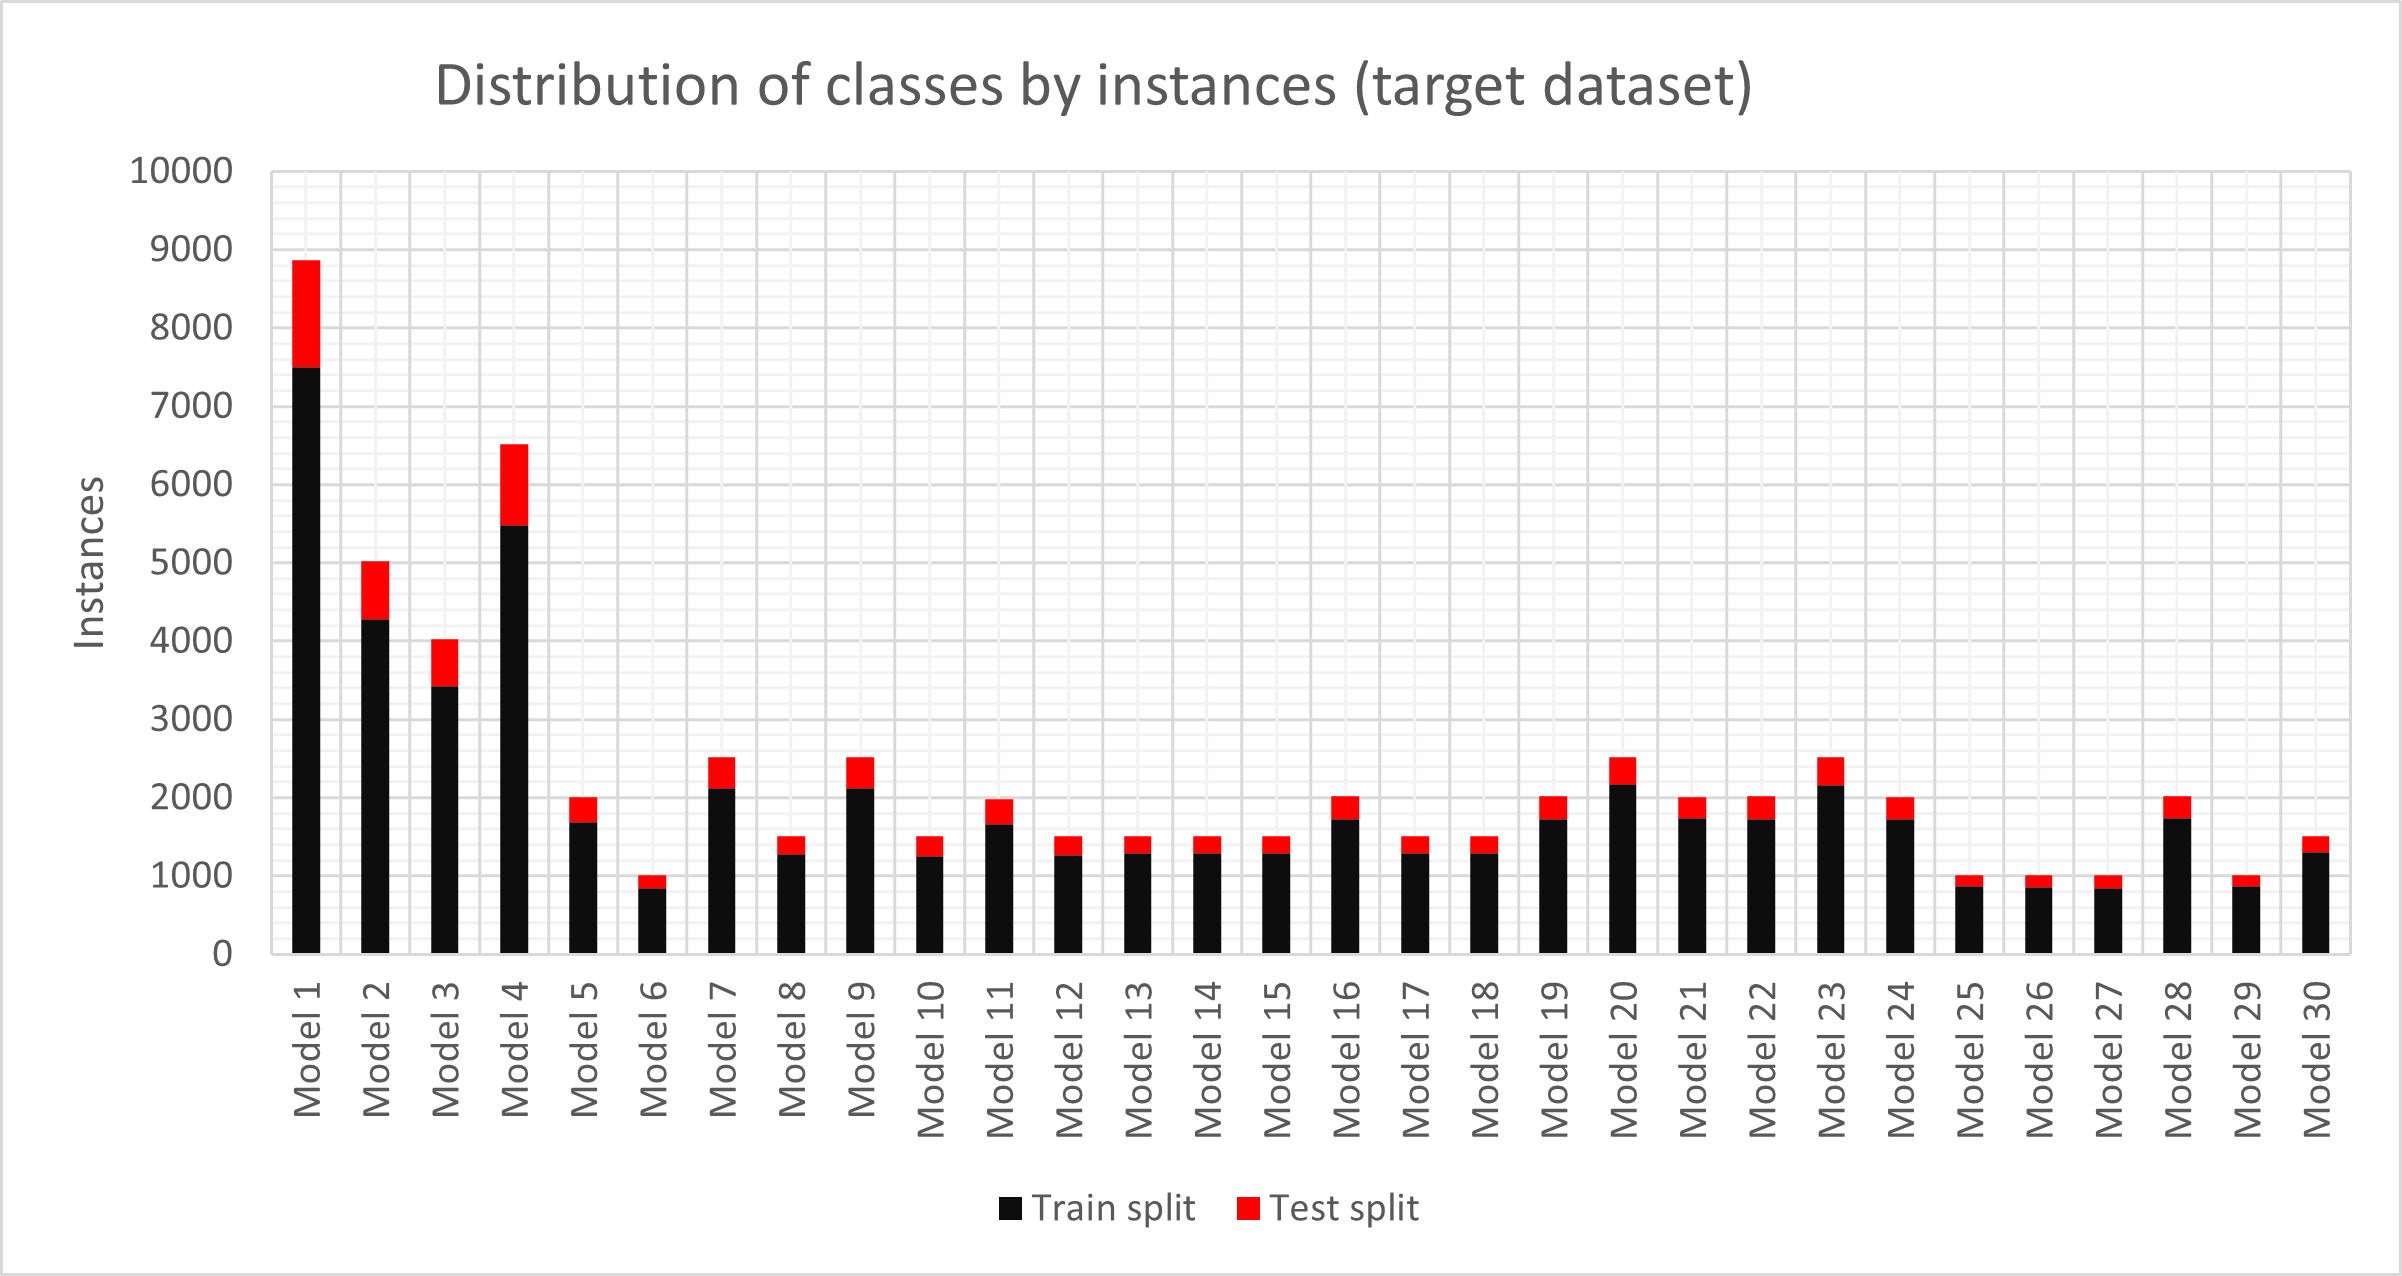
\includegraphics[width=14cm]{./real_distribution.png}
	\end{center}
	\caption{Distribution of the classes in the real subset of T-LESS dataset. Total number of object instances: 10362}
	\begin{center}
		\label{tless_distribution_real}
	\end{center}
\end{figure}
\FloatBarrier

\subsection{Preliminary experiments}
In the long term, the idea behind the project is to implement a scalable system that would identify real-life images of the equipment given the 3D images from the simulator. Therefore, as a default setup it was decided to use the rendered T-LESS-based dataset for training, and the real T-LESS-based dataset for evaluation. Naturally, in object detection problems, choosing the right detector is just as important as preparing the dataset. For the initial experiments, Faster-RCNN  \cite{Girshick2015} model was tested.

Additionally, YOLOv3 \cite{Redmon2018a} was considered. However, unlike Faster-RCNN, YOLO has not been as popular, according to Figure \ref{popularity}. This was partially due to flexibility of Faster-RCNN when it comes to replacing different components of the network in order to improve the results. Although YOLO proved to be significantly faster than Faster-RCNN as discussed earlier in the \nameref{yolo_section} section, in this thesis, the flexibility of the network and its accuracy are treated  as higher priority tasks. For these reasons, Faster-RCNN will be used in all further experiments.  
   

\subsubsection{Metrics}
\label{metrics_section} 

As for the detection evaluation, here and in the further experiments and in order to match the selected dataset format, the metrics were employed in accordance with the mean average precision metric(mAP) of the PASCAL VOC \cite{Everingham10} challenge. In order to measure the mAP, first the parameters should be calculated in the confusion matrix. Confusion matrix is a generic performance measurement tool in ML. According to PASCAL VOC, precision and recall are the most important terms in object detection tasks that can be extracted from the confusion matrix. The equations for precision and recall are outlined in Table \ref{confusion}.

\todo{Update this citation as suggested by Christian} 
\begin{table}[htb]
	\captionof{table}{Definition of confusion matrix and some of its terms, adapted from \cite{mAp_blog}.}
	\begin{center}
		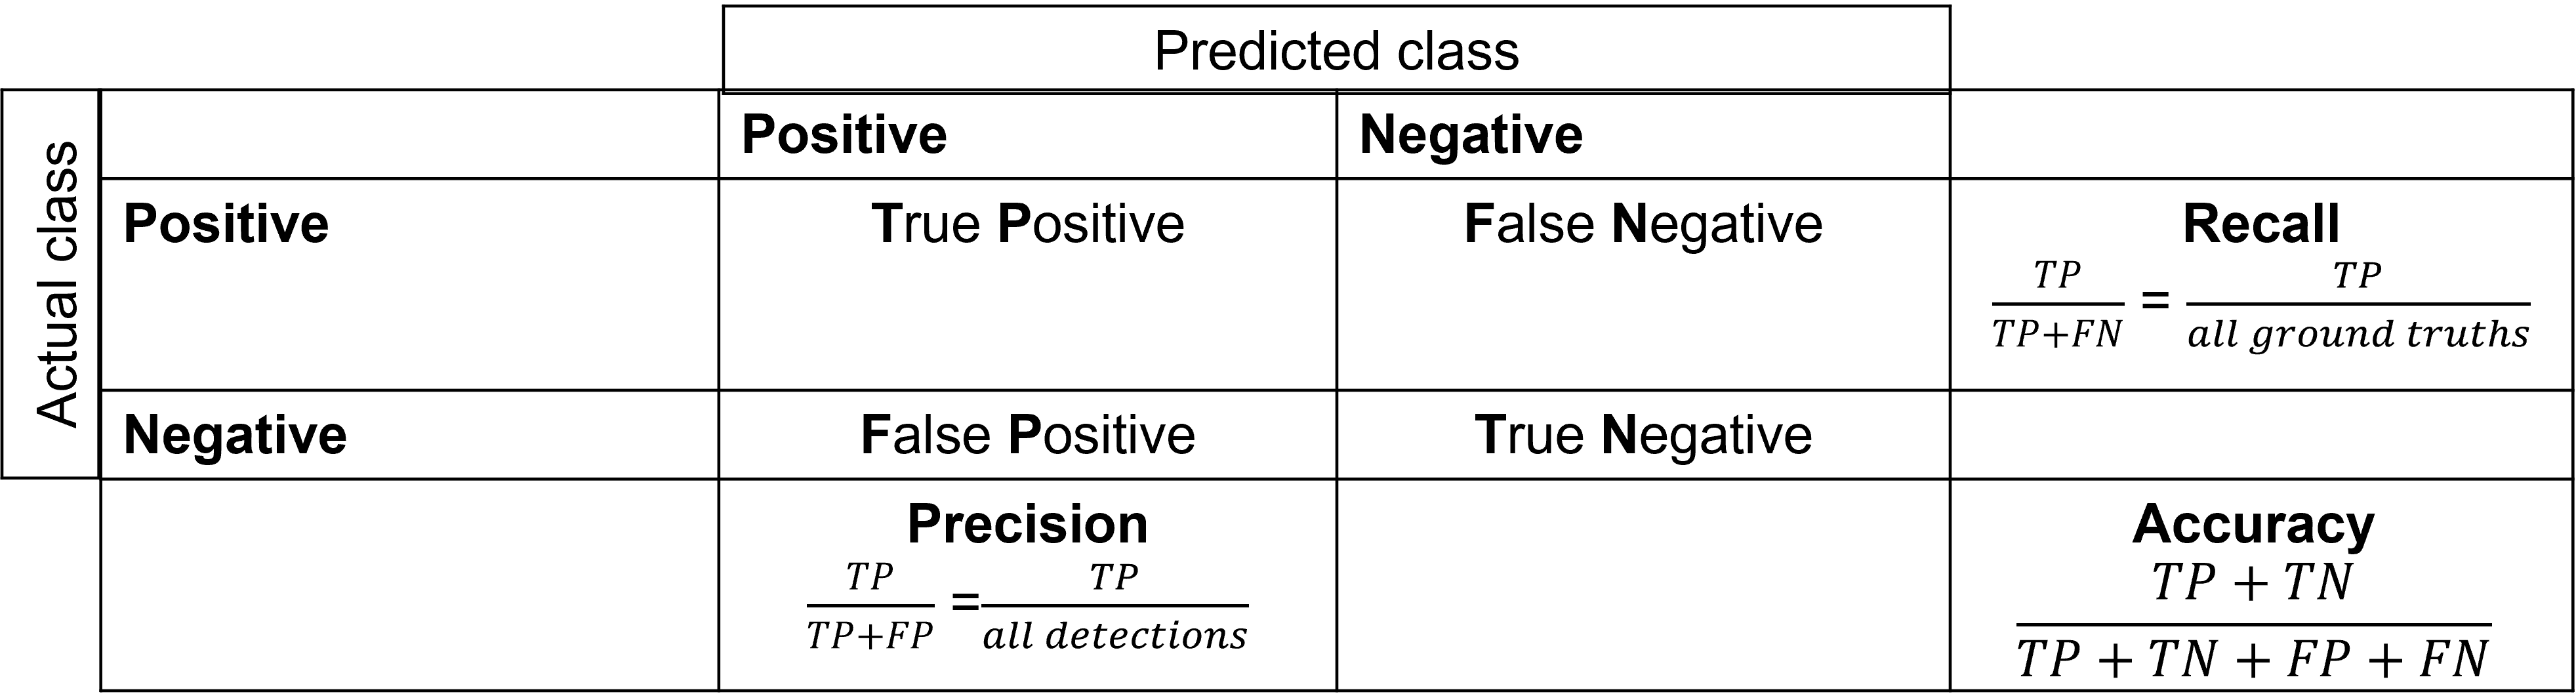
\includegraphics[width=14cm]{./confusion.png}
	\end{center}
	\begin{center}
		\label{confusion}
	\end{center}
\end{table}
\FloatBarrier

\todo{add the IOU image that was used in the presentation} 
To calculate precision and recall, it is important to define how the True Positive (TP) term is calculated. Unlike, in image classification tasks, this calculation is not as straightforward. Since the objects need to be localized correctly as well as identified, comparing ground-truth labels against the predicted classes is not enough. This issue was addressed in COCO challenge \cite{Lin2014} by measuring the Intersection-over-Union (IoU) metric. As the model proposes an anchor box, the classifier outputs a confidence score. The confidence score is a probability of the box to contain an object. The region is then additionally compared against the ground truth bounding box labels using the Equation \ref{iou}. Finally, if the IoU ratio, also known as Jaccard distance, is above the pre-defined threshold, the predicted object is considered to be a TP. In PASCAL VOC evaluation, the default threshold is 0.5 \cite{mAp_blog} and only predictions with the highest confidence scores count. 

The prediction is labeled as False Positive(FP) when either the predicted class is wrong or its IoU is below the threshold. Otherwise, if the confidence score of the proposed region is lower than the threshold, the value is labeled as False Negative(FN). Next, precision and recall values are calculated as specified in Figure \ref{confusion}.

\begin{equation}
\operatorname{IoU}\left(\text { Area }_{\text {Prediction }}, \text { Area }_{\text {Ground truth }}\right)=\frac{\mid \text { Area }_{\text {Prediction }} \cap \text { Area }_{\text {Ground truth }} \mid}{\mid \text { Area }_{\text {Prediction }} \cup \text { Area }_{\text {Ground truth }} \mid}
\label{iou} 
\cite{mAp_blog} 
\end{equation}

The area under the Precision-to-Recall curve is known as Average Precision(AP). The pairs of precision and recall are recorded at multiple confidence scores and compared against each other in the Precision-to-Recall curve. In PASCAL VOC 2010-2012 \cite{Everingham10}, the area under the curve is smoothed first, and then the rectangles below the interpolated curve are summed as shown in Figure \ref{AUC}. The interpolation $p_{\text {interp }}$ of the curve $p$ is performed using Equation \ref{interp}, where $r$ is a recall level. 

\begin{figure}[htb]
	\begin{center}
		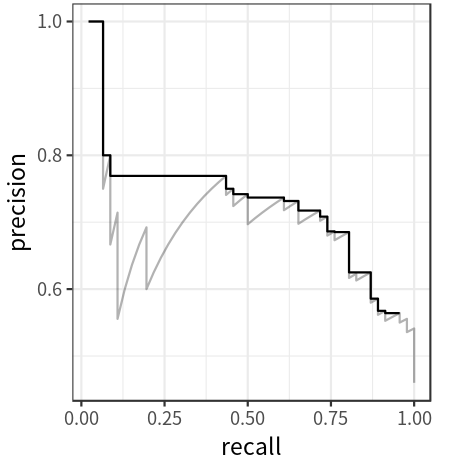
\includegraphics[width=12cm]{./AUC.png}
	\end{center}
	\caption{Average precision curve \cite{mAp_blog}.}
	\begin{center}
		\label{AUC}
	\end{center}
\end{figure}
\FloatBarrier


\begin{equation}
p_{\text {interp }}(r)=\max _{r^{\prime} \geq r} p\left(r^{\prime}\right)
\label{interp}
\cite{mAp_blog}  
\end{equation}

In the subsequent sections, \texttt{AP50} and \texttt{AP75} denote average precision at IoU of 0.5 and 0.75, respectively, as defined by COCO \cite{Lin2014}. According to PASCAL VOC \cite{Everingham10} evaluation methods, \texttt{AP} stands for average precision at all confidence intervals, unlike COCO \cite{Lin2014} and earlier iterations of PASCAL VOC, where \texttt{AP} was only calculated at 11 equally spaced fixed intervals. In the following sections, the terms mAP and \texttt{AP} will be used interchangeably. Finally, in all the experiments listed in this thesis, \texttt{AP50} will be the primary metric for evaluation of a method.  


\subsubsection{Naive object detection approach}
\label{naive} 
Due to the simplicity of setup, Faster-RCNN \cite{ima} was selected as  candidate for object detection pipeline. In this setup, Faster-RCNN detector in Detectron2  \cite{wu2019Detectron2} was applied to the dataset presented in the \nameref{datasets} section. 

For the initial experiments, a Faster-RCNN network with a ResNet backbone was used as it was concluded to be the best among the networks listed in the section \nameref{classification_section}. The ResNet architecture had 50 layers. The training has been conducted in three stages. First, the model was trained on the source dataset. Next, the trained model was evaluated on the real images of the same classes. Finally, an identical model has been trained on the target dataset for comparison. The evaluation in all three stages followed the metrics outlined in the section \nameref{metrics_section}. After training the model for a short duration, corresponding to 20 000 iterations and the base LR of 0.00125, it quickly became evident that the solution has to be more complex in order to solve the challenges outlined in the \nameref{objective}. The results of the initial experiments are shown in Figure \ref{faster_init}.


\begin{table}[htb]
	\captionof{table}{Experiments with a simple Faster-RCNN model. }
	\begin{center}
		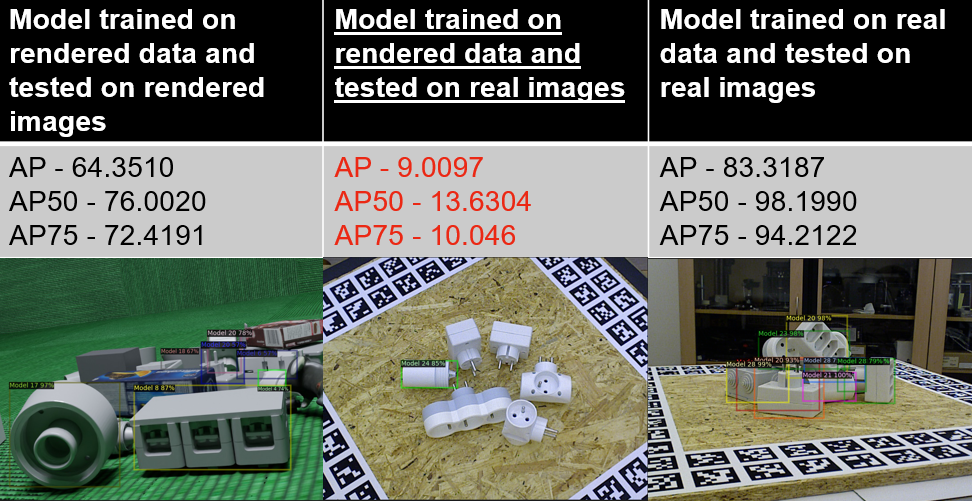
\includegraphics[width=14cm]{./initialExp.png}
	\end{center}
	\begin{center}
		\label{faster_init}
	\end{center}
\end{table}
\FloatBarrier

As it can be concluded, there is a significant performance drop when the environment is slightly changed. This is essentially a result of two related problems combined: over-fitting and domain shift. Naturally, the regular detector fails when two datasets originate from different environments and not only their background, but also their lighting conditions, positioning and textures deviate from one another. Moreover, because the target dataset is substantially smaller, there is a chance that the model overfits in the third training stage. To conclude, it is believed that with right hyperparameters and a carefully refined training  process with longer training time, the results can be improved, though not significantly. 

\subsubsection{Experiments with classical domain adaptive methods}
To overcome the domain shift phenomenon, it was proposed to experiment with domain adaptation applications. For these experiments, two existing open-source methods were suggested. 

In the initial study, a model based on decoupled adaptation for cross-domain object detection \cite{Jiang2021} was tested. The model introduced by Jiang et al. essentially proposes an \nameref{adv_approach} approach, where a GRL is applied to the classifier and the box regressor in a decoupled way, i.e. the problem is split into two sub-problems to avoid them from interfering with each other. According to Jiang et al., this could improve the discriminability of the detector. Readers can refer to the original paper \cite{Jiang2021} for more information. The results of the experiments are outlined in the Table \ref{dadapt}.

\begin{table}[htb]
	\captionof{table}{Results of the experiments with a D-Adapt based method.}
	\begin{center}
		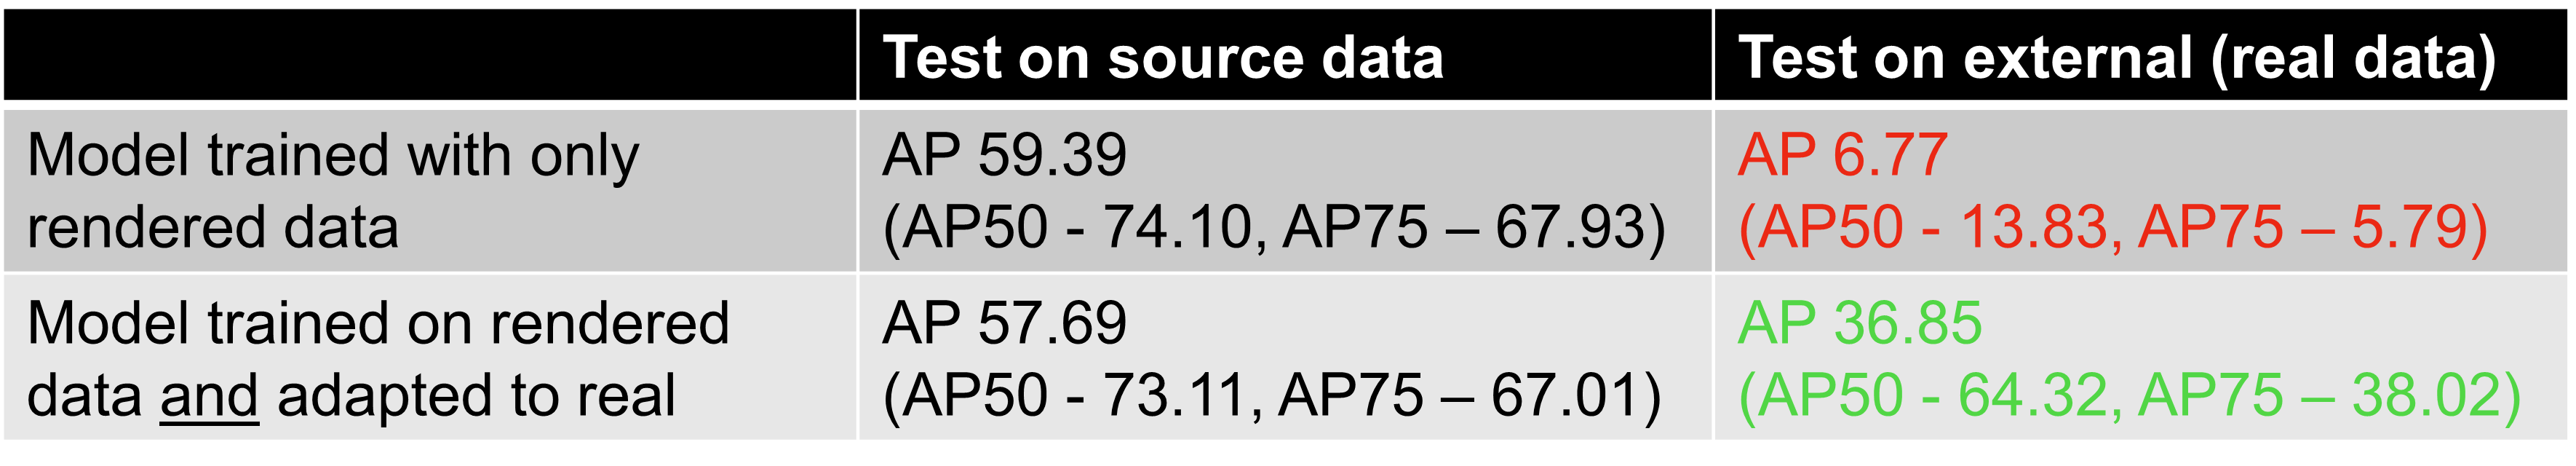
\includegraphics[width=14cm]{./dadapt.png}
	\end{center}
	\begin{center}
		\label{dadapt}
	\end{center}
\end{table}
\FloatBarrier

First, a model was trained on the source dataset for 4 hours. Similarly to the \nameref{naive}, the performance drops dramatically when testing the model on the target dataset. However, after running the adaptation network for another 4 hours, the results have improved by a considerable margin. The final result on the combined dataset is \texttt{AP50} $= 64.32\%$. The result has significantly improved over the experiment without any adaptation presented in Table \ref{faster_init} with \texttt{AP50} $= 13.63\%$. 

Recently, many open-source solutions proposed \cite{Inoue_2018_CVPR, Chen2020, Arruda2019} an \nameref{imagetoimage} approach in a cross-domain object detection setup. Following Zhu et al., Cycle-GAN \cite{Zhu2017} was used in an attempt to generate an intermediate domain. The results obtained after training the model for 44 epochs(= 36 hours) are compiled in Table \ref{cyclegan}.  

\begin{table}[htb]
	\captionof{table}{Results of the experiments with Cycle-GAN}
	\begin{center}
		\includegraphics[width=16cm]{./cyclegan.png}
	\end{center}
	\begin{center}
		\label{cyclegan}
	\end{center}
\end{table}
\FloatBarrier

As it can be noted, even after an extensive training with a massive dataset of nearly 50 000 images, Cycle-GAN still produced fairly low-quality results, especially for the real-alike images. This problem has also been acknowledged by Zhu et al. as a limitation of Cycle-GAN \cite{Zhu2017}, where differences in the distribution characteristics of the training dataset caused similar artifacts. Due to the low performance on the T-LESS dataset and long training time, this method was excluded from further tests. 


\subsection{Experiments with Adaptive teacher}
\label{ensemExp} 
For the next set of experiments, this thesis proposes an ensembled setup. An ensembled setup is a combination of multiple algorithms that leverage their benefits to produce a superior result. In regards to domain adaptive object detection, such setups were summarized earlier in the \nameref{mean_teacher} section. As a base study for this thesis, the adaptive teacher \cite{Li2021}  framework is studied extensively. Unlike the  previous architectures, mean teacher training frameworks implement multiple adaptation strategies. In case of the adaptive teacher method, Li et al. proposed to use both adversarial and pseudo-labeling techniques. To validate the suitability of this architecture, the code base has been modified to accept the prepared T-LESS dataset and was trained as it is. Figure \ref{adapt_experiment1} illustrates the results when visualizing the trained model. Similarly, to the previous experiments, the model was based on Faster-RCNN \cite{ima} and a ResNet \cite{He2015} backbone network with 101 layers, which was pre-trained on the ImageNet  \cite{Russakovsky2014} dataset. Although traditional ML and DL algorithms utilize the term epoch, which stands for one forward and one backward passes of the loop for the entire set of the training samples, Detectron2 \cite{wu2019Detectron2} uses the term "iterations" instead. Iterations denote a number of times to complete the forward and backward passes for a batch of training samples, where a batch is a small subset of data. 

\begin{figure}[htb]
    \centering
    \subfloat[Visualization on the source dataset]{{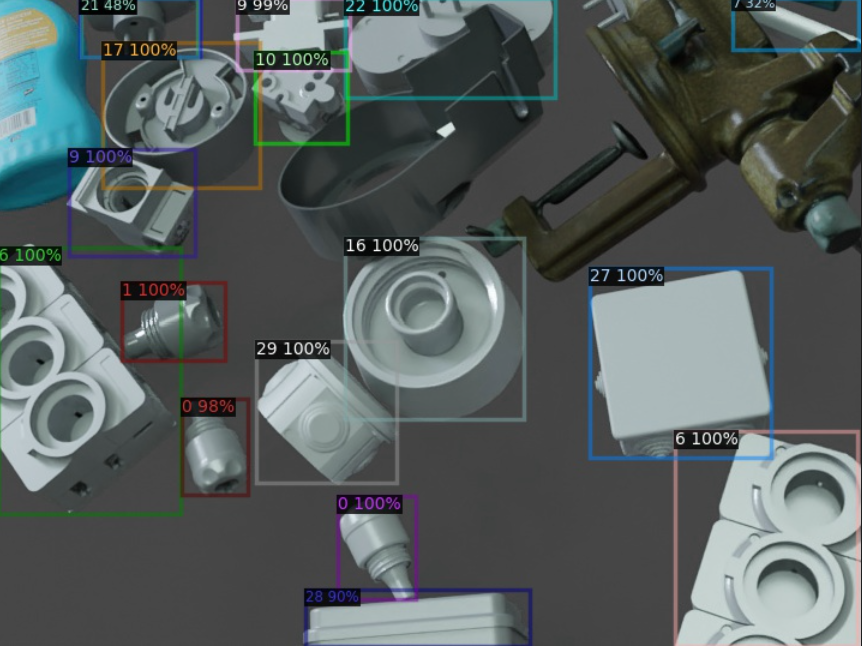
\includegraphics[width=6cm]{./experiments_original_1.png} }}%
    \qquad
    \subfloat[Visualization on the target dataset]{{\includegraphics[width=6cm]{./experiments_original_2.png} }}%
    \caption{Results of the experiments with Adaptive Teacher as it is}\label{adapt_experiment1}%
\end{figure}
\FloatBarrier

Expectedly, the model performs poorly on the custom dataset without tweaking any hyperparameters. Although the performance on the source dataset is more than satisfactory (Figure \ref{adapt_experiment1} (a)), random artifacts take place in the form of noisy bounding boxes, as can be seen in Figure \ref{adapt_experiment1} (b). For this round of experiments, the number of iterations was set as high as possible in order to explore the limits of the setup. Although the model was trained for 360 000 iterations, such huge values are often redundant as the selected dataset has extensive amount of images and, therefore, less iterations can be used, as will be presented in \nameref{results}. 
\todo{perhaps convert iterations to epochs} 

To overcome the issue of noisy predictions, two steps have been carried out. First, the LR scheduler has been adjusted in the original Adaptive teacher \cite{Li2021} implementation. In the original setup, the Adaptive teacher algorithm used a warm-up two-stage multi-step scheduler. This scheduler initializes the LR in two stages, where it first gradually increases for a number of warm-up iterations $\texttt{WARMUP\textunderscore ITERS} = 1000$, until it reaches the fixed $\texttt{BASE\textunderscore LR} = 0.001$.  Instead, this thesis suggests to use the multi-stage scheduler with a cosine annealing, as suggested by Loshchilov et al. \cite{Loshchilov2016}. In these experiments, the learning rate first slowly ascends to the $\texttt{BASE\textunderscore LR} = 0.001$. However, as the ceiling is reached, it starts to decay to zero by the time of the last iteration $\texttt{MAX\textunderscore ITERS}$ is reached. This in theory allows to protect the scheduler from overshooting as it approaches the global minimum. Although Loshchilov et al. additionally proposes resetting the scheduler after it reaches the minimum, in this thesis such implementation is neglected for the time being. Both schedulers are compared against each other and are illustrated in Figure \ref{annealing}.

Another issue that potentially caused the noisy predictions on the real images is over-fitting. This might happen when, given the model complexity, the model is trained for an excessive amount of time. As a result, the model would only perform well on the training data. 
Therefore, in order to identify the suitable number of iterations required for training, an early stoppage algorithm was added. Instead of checking whether the loss keeps decreasing, the \texttt{AP50} metrics is tracked for the validation set at every \texttt{EVAL\textunderscore PERIOD} interval. If the value does not improve for more than $\texttt{EVAL\textunderscore PERIOD} \times \texttt{PATIENCE}$ iterations, the best model is saved and the training is terminated. The results of such modification are presented later in the \nameref{results} section.  

\begin{figure}[htb]
	\begin{center}
		\includegraphics[width=14cm]{./LR.jpg}
	\end{center}
	\caption{a) The original LR scheduler against b) The proposed cosine annealing LR scheduler without restarts}
	\begin{center}
		\label{annealing}
	\end{center}
\end{figure}
\FloatBarrier

\subsection{Regularized Cross-Domain Adaptive Teacher}
\label{mainExperiments} 
In the subsequent sections, a novel architecture will be introduced. The effectiveness of the existing methods has been evaluated to address domain shift  between various open-source datasets. Most often domain adaptation is performed to transfer knowledge from one dataset for autonomous driving(Cityscapes) to another(Foggy-Cityscapes, Sim10k, KITTI), or to transfer knowledge from one dataset with general objects (PASCAL VOC) to another(Clipart, Watercolor, Clipart) \cite{Oza2021}.  

However, no comprehensive work have addressed the industrial cross-domain object detection. Additionally, motivated by works of Li et al. \cite{Li2021} and Xu et al. \cite{Xu2020}, this thesis assesses the practicality of the categorical regularization in the adaptive teacher framework. Unlike the original architecture of Adaptive teacher \cite{Li2021}, the model is aligned at two stages:  image-level and instance-level. Following Chen et al. \cite{Chen2018} and Xu et al. \cite{Xu2020}, a consistency loss term has been added to regularize both stages. The training process follows similar principles to the ones outlined in the \nameref{ensemExp} section. The proposed architecture is presented in Figure \ref{mymodel}. 

\begin{figure}[htb]
	\begin{center}
		\includegraphics[width=16cm]{./MyModel.png}
	\end{center}
	\caption{A proposed architecture for cross-domain object detection. Blue elements represent standard Faster-RCNN components, purple elements - domain adaptation components and yellow elements are Faster-RCNN modified components for continual learning, which will be discussed later.}
	\begin{center}
		\label{mymodel}
	\end{center}
\end{figure}
\FloatBarrier

Chen et al. \cite{Chen2018} was one of the first methods to use a two-level alignment, which was discussed earlier in the \nameref{adv_approach} section. Xu et al. \cite{Xu2020} expanded further on this method by adding a consistency regularizing term. Upon analyzing multiple papers, Xu et al. comments that using only image-level adaptation would result in the alignment of the non-transferable background regions between the source and target domains, which would in turn result in poor accuracy in the target domain \cite{Xu2020}. Instance-level alignment would allow to reduce the distance between the local features, such as object appearance, size and viewpoint \cite{Chen2018}. On the other hand, it is not possible to omit image-level alignment as it is important to address adaptation of the global features of the image, such as image scales, illumination and style \cite{Chen2018}. 

Therefore, this setup employs a mean teacher based Faster-RCNN \cite{ima} setup with two domain adaptation networks in the student model. Similarly to the preceding architectures \cite{Li2021,Liu2021}, data augmentation is used to assist in the training process, For these experiments, random cropping was excluded from tests as it was negatively affecting the pseudo-labeling. Instead, a few other transformations such as histogram equalizing and sharpness adjustments, were added to strong augmentation. The complete list of used augmentations is shown in Figure \ref{newAugmentations}. It is believed that rotations and random affine transformations are not as important with the T-LESS dataset as the number of images taken in a rotational manner seems to be fairly sufficient.

\begin{figure}[htb]
	\begin{center}
		\includegraphics[width=16cm]{./Tless_augm.png}
	\end{center}
    \caption{Augmentations used in the experiments.}
	\begin{center}
		\label{newAugmentations}
	\end{center}
\end{figure}
\FloatBarrier

Identically to the earlier experiments, the backbone was chosen to be ResNet \cite{He2015} with 101 layers. Following Li et al. \cite{Li2021}, one adaptation module is attached to the output of a CNN backbone.  Another domain adaptation network is attached to the output layers of Faster-RCNN. While the backbone generates image-level features, Faster-RCNN outputs the proposed foreground regions. Both modules utilize a standard GRL block \cite{Ganin2015} followed by a domain classifier.



In this work, the image-level domain classifier is similar to the basic CNN architecture illustrated in Figure \ref{CNN} and it was defined in accordance with the setup of Li et al. \cite{Li2021}. It has three convolutional layers with batch normalization and leaky-ReLUs followed by a convolutional classier layer. The instance-level classifier resembles the architecture in \cite{Xu2020} and consists of two linear layers with leaky-ReLUs and dropout layers and finalized with a classifier and a sigmoid. Dropout layers were added due to the reasons specified in Section \ref{alexnet_section}. A detailed description of the architecture can be found in the \nameref{appendix}. 

Naturally, both an image and a region proposed by Faster-RCNN should represent the same domain. Similarly to Xu et al., to minimize the difference between predictions of the domain classifiers, they are regularized using $\mathcal{L}_{\text {consist }}$ consistency loss. In these experiments, consistency loss is based on simple MSE loss between instance- and image-level domain classifier loss terms $\mathcal{L}_{\text {ins }}$ and $\mathcal{L}_{\text {img }}$, as it was described in Equation \ref{MSE_eq}.

The calculations of both $\mathcal{L}_{\text {ins }}$ and $\mathcal{L}_{\text {img}}$ follow the practices outlined in Equation \ref{faster_DA_losses}. Additionally,  the consistency loss $\mathcal{L}_{\text {consist }}$ follows the formula in Equation \ref{faster_DA_losses_consist}. However, instead of L2 norm, MSE is utilized.  

To trade-off between different loss parameters, the weights of the domain classification and consistency losses have been added to the original setup of the Adaptive teacher network. The complete formula for loss computation is displayed in Equation \ref{total_loss}. 

\begin{equation}
\mathcal{L}=\mathcal{L}_{\text {sup }}+\lambda_{\text {unsup }} \cdot \mathcal{L}_{\text {unsup }}+\lambda_{\text {img }} \cdot \mathcal{L}_{\text {img }}+\lambda_{\text {ins }} \cdot \mathcal{L}_{\text {ins }}+\lambda_{\text {consist }} \cdot \mathcal{L}_{\text {consist }},
\label{total_loss} 
\end{equation}

where $\mathcal{L}_{\text {sup }}$ is the standard Faster-RCNN detector loss in the student model; $\mathcal{L}_{\text {unsup }}$ is the unsupervised loss between pseudo-labels generated by the teacher model and supervised predictions and the $\lambda$-s are the corresponding hyper-parameters to regularize the weights of different loss terms. The $\mathcal{L}_{\text {sup }}$ is calculated in a similar manner as it was introduced earlier in Equation \ref{faster_rcnn_loss}. 
 
Pseudo-labels for the unlabeled target dataset are obtained identically as in \cite{Li2021}. The noisy pseudo-labels are filtered using a confidence threshold and a class-wise NMS \cite{Liu2021}. These pseudo-labels are considered as a ground-truth in the calculation of the unsupervised loss $\mathcal{L}_{\text {unsup }}$. It is essentially based on a standard Faster-RCNN loss. However, it does not include the bounding box regression loss, as it not possible to filter out the bounding boxes using only confidence threshold, which was specified by Liu et al. \cite{Liu2021}.  Instead, to improve the quality of pseudo-labels, EMA is applied to gradually move weights from the student to the teacher model as discussed in the  \nameref{mean_teacher} section, and it is the only place where updating the teacher model takes place \cite{Li2021}.  
 
Multiple experiments have been conducted with the architecture defined in Figure \ref{mymodel}. These experiments will be discussed in the \nameref{results} section.  

In the following section, a proposed continuously learning domain adaptative object detection setup is introduced. 


\subsection{Object detection with continual learning}
\label{cont_learning_section} 
Although the pre-trained model performs fairly well on the target dataset, it will not be able to predict unknown objects. In order to solve the scalability problem defined in the \nameref{objective}, the proposed architecture should be able to keep learning when new data is added. Often such problems are addressed by a special case of transfer learning known as "fine-tuning". A typical example of fine-tuning is done by freezing certain deeper layers and only retrain the top level components of the network. This procedure would enable the network to apply previously learned knowledge on an unknown yet similar problem, while significantly reducing the training time. In regards to the objectives of this thesis, it would allow to utilize the knowledge of the previously learned equipment parts to promptly retrain it and apply it to new classes of objects. 
In the first set of experiments, a naive fine-tuning approach without freezing was attempted. The model was trained based on the architecture, which was demonstated in the \nameref{mainExperiments}. The regular training stage included both source and target datasets that contained classes 1 to 20, while the fine-tuning stage only included the data for classes 21-30 and the pre-trained weights file from the previous stage. After the model has been trained on the first 20 classes, the FC layers of the trained model have been removed and replaced with new FC layers that can produce predictions for 30 classes. Both models were trained for the same number of iterations. The results are presented in Table \ref{naive_finetuning}.

\begin{table}[htb]
\caption{The naive fine-tuning results}
\label{naive_finetuning}
\resizebox{\textwidth}{!}{%
\begin{tabular}{l|l|l|ll}
\cline{2-3}
                                         & Model trained on data from classes 1-20      & Model trained on data from classes 21-30   &  &  \\ \cline{1-3}
\multicolumn{1}{|l|}{Base learning rate} & 0.001                              & 0.0005                           &  &  \\ \cline{1-3}
\multicolumn{1}{|l|}{Outputs}            & Predictions for 20 classes         & Predictions for 30 classes       &  &  \\ \cline{1-3}
\multicolumn{1}{|l|}{Max iterations}     & 35000                              & 35000                            &  &  \\ \cline{1-3}
\multicolumn{1}{|l|}{Training time}      & about 8 hours                      & about 8 hours                    &  &  \\ \cline{1-3}
\multicolumn{1}{|l|}{Data} &
  \begin{tabular}[c]{@{}l@{}}source (labeled) and target (unlabeled) \\ datasets limited to classes 1-20\end{tabular} &
  \begin{tabular}[c]{@{}l@{}}Saved weights(.pth) from the original model(1-20) \\ + datasets limited to classes 21-30\end{tabular} &
   &
   \\ \cline{1-3}
\multicolumn{1}{|l|}{Results}            & \textbf{AP} 58.1596, \textbf{AP50} 75.27, \textbf{AP75} 66.89 & \textbf{AP} 19.93, \textbf{AP50} 29.78, \textbf{AP75} 22.36 &  &  \\ \cline{1-3}
\end{tabular}%
}
\end{table}

As can be easily noted, the results dropped significantly even though the initial weights are supposed to give a decent advantage. This setup would not only have low performance on the new data, but also unable to classify and localize original dataset. A few important modifications were considered in the next experiment: 

\begin{enumerate}
\item In order to fine-tune the network successfully, a freezing process should be carried out on the deeper, more specifically, on the backbone layers of the network. Skipping this step is the main result of the performance drop in Table \ref{naive_finetuning}. By freezing deeper parts of the network, key trained features will be preserved, and the number of trainable parameters will be reduced, which will in turn speed up the training time. 
\item Too many unfamiliar cases will lead to a higher performance drop. Adding fewer additional classes in each subsequent task will help to maintain the performance drop at the lower level. This has been proven by experiments of Peng et al. \cite{Peng2020}. In other words, instead of retraining the original model with 10 more unknown classes, the model should be retrained with one or two at most. 
\item Additionally, the weights file \texttt{.pth}, which was originally trained for the first $N$ classes, also contained the states of the optimizer, i.e. of the training process. This included the iteration number and the learning rate at that iteration. As a result, the training process is started from a much lower base LR. Therefore, before proceeding, the optimizer states were removed from the dictionary of the weights file. 
\item Finally, instead of replacing the original FC layers altogether, a new architecture is proposed, as illustrated in Figure \ref{continualModel} (b). 
\end{enumerate}

Following the studies presented in the \nameref{cont_learning} section, the detector head of the custom model is additionally modified to address a scalable training setup. The architecture presented in Figure \ref{continualModel} (b) replicates the method proposed by Rusu et al. \cite{Rusu2016}, but in a cross-domain mean teacher setup. An overview of this method was shown earlier in Figure \ref{mymodel}, where both detector heads of the student and the teacher networks are modified. In this experiment, the original detector head is frozen, which includes both the classifier and the box regressor. Freezing essentially prevents the weights from being modified by disabling the learning rate updates. Consequently, new output layers are attached to the network. These layers are responsible for the unknown $M$ number of classes and unlike the original detector, they are not frozen. The original detector head classifies an $N+1$ number of objects, which also includes the background. Therefore, to preserve data integrity, the appended detector head ignores the background class and only predicts $M$ new objects. 

One potential disadvantage to such approach is that the original detector head is trained to recognize the background as well, which also included the shapes of the new $M$ objects. Moreover, the weights for the original detector are frozen. Therefore, it is believed that the appended detector head will struggle predict the new classes if the original detector forces it to be predicted as "background". 

To solve this problem, a new architecture has been introduced in Figure \ref{continualModel} (c). This model further combines the ideas proposed by Rusu et al. \cite{Rusu2016} and Donahue et al. \cite{Donahue2013}, which were introduced in the \nameref{cont_learning} section. Instead of completely freezing the original detector weights, the learning rate is reduced for the previously trained objects. The additional FC layers are trained with a standard LR.  According to Parisi et al. \cite{Parisi2018}, reduced learning rate will prevent the model from making significant changes in the original weights, while also learning new data. This might potentially enable the network to slowly be re-trained and learn the difference between the new classes and the background. Meanwhile, the dynamically expanding architecture of Rusu et al. \cite{Rusu2016} will focus on fighting the catastrophic forgetting problem. Ultimately, in the proposed method the model aims to train network expansion along with regularization. 

The results of such architecture are summarized in the \nameref{cont_learning_results} section. 


\begin{figure}[htb]
	\begin{center}
		\includegraphics[width=16cm]{./FC.png}
	\end{center}
	\caption{A proposed architecture for continual learning setup. Blue elements represent standard Faster-RCNN components, yellow elements are modified components for continual learning.}
	\begin{center}
		\label{continualModel}
	\end{center}
\end{figure}
\FloatBarrier


\clearpage 


\section{Results} 
\label{results} 
This section summarizes the key findings of the experiments that were conducted based on the architectures presented in the sections \ref{ensemExp},  \ref{mainExperiments} and \ref{cont_learning_section} of the thesis. Additionally, this section briefly introduces the simplistic UI and evaluates the proposed model on one equipment item from a real plant. 

\subsection{Cross-domain adaptation results}

In order to achieve fair comparison, all experiments obey the following specifications:
\begin{enumerate}
\item The results presented in the subsequent sections will be evaluated predominantly on the T-LESS dataset as introduced in the \nameref{datasets} section. 
\item Thirty objects in the dataset were given arbitrary class names using the following notation: \texttt{Model 1..Model 30}
\item According to the setup defined in Figure \ref{mymodel}, the \underline{teacher model} accepts only the weakly-augmented images from the \underline{target} domain. The primary objective of the model is to improve performance on the target images. Therefore, the primary objective for this ensembled model is to improve the \texttt{AP} on the teacher model. Thus, \texttt{AP50} metrics are recorded for the target images and are then used for comparison. 
\item The base learning rate is defined as \texttt{BASE\textunderscore LR} = 0.001.
\item The number of iterations is fixed at \texttt{MAX\textunderscore ITER} = 50 000.
\item The evaluation happens every \texttt{EVAL\textunderscore PERIOD} = 1000 iterations. Considering that there are 50 000 iterations total, this results in 50 evaluation points across the \texttt{AP50} plot.
\end{enumerate}  

\subsubsection{Scheduler adjustment}
\label{scheduler_section} 
First set of experiments was conducted in accordance with the \nameref{ensemExp} section.  For the baseline comparison, the Adaptive Teacher network was initially trained as it is. This implies that no external components were added and the original learning rate scheduler was used. The pattern of the original scheduler was presented earlier in Figure \ref{annealing} (a). The results of such setup are presented in Figure \ref{original_experiment}. The first graph illustrates the evaluation \texttt{AP50} results for both the teacher and the student models. Although the training process seems idle for the first 20 000 iterations, the model eventually finds better gradients and stabilizes at $max$ (\texttt{AP50}) = 71.40 \% at 31 000 iterations. Even though it might seem that the loss value is decreasing by the end of the training, the \texttt{AP50} value also steadily drops. In order to address the noisy predictions shown earlier in Figure \ref{adapt_experiment1}, the learning rate scheduler has been modified to implement a cosine annealing algorithm without restarts \cite{Loshchilov2016}, as shown in Figure \ref{annealing} (b). The original warm-up period of \texttt{WARMUP\textunderscore ITERS} = 1000 is preserved. 

\begin{figure}[htb]
	\begin{center}
		\includegraphics[width=16cm]{./loss&AP50_original.jpg}
	\end{center}
	\caption{Results of the original Adaptive Teacher model evaluated on the custom T-LESS dataset without any modifications.}
	\begin{center}
		\label{original_experiment}
	\end{center}
\end{figure}
Theoretically, this setup would have allowed to find better gradients and reduce overshooting. The results achieved after modifying the scheduler are shown in Figure \ref{comparison_1}. Although the \texttt{AP50} value peaked much faster with the new scheduler, it was only able to reach $max$ (\texttt{AP50}) = 62.50 \%, which is almost 10 \% lower than the original result.   

\begin{figure}[htb]
	\begin{center}
		\includegraphics[width=14cm]{./AP50_scheduler.jpg}
	\end{center}
	\caption{a) \texttt{AP50} results of the original model and b) \texttt{AP50} results of the model with a cosine scheduler.}
	\begin{center}
		\label{comparison_1}
	\end{center}
\end{figure}
\FloatBarrier

\subsubsection{Additional augmentations}
\label{augmentations_section} 
Following the ideas proposed in Figure \ref{newAugmentations}, an identical model was trained with two additional strong augmentations. This in theory allows to further diversify the dataset, which will make it less prone to over-fitting. Furthermore, in this and the subsequent  experiments, the model leverages the early stopping algorithm with the parameter of $\texttt{PATIENCE} = 10$. The early stopping algorithm will prevent the model from unnecessary training in case if the \texttt{AP50} does not improve for more than $\texttt{PATIENCE} \times \texttt{EVAL\textunderscore PERIOD} = 10 000$ iterations. The results of the evaluation process with the additional augmentations can be found in Figure \ref{augmentation_experiment}. 
 
\begin{figure}[htb]
	\begin{center}
		\includegraphics[width=14cm]{./AP50_augmentation.jpg}
	\end{center}
	\caption{a) \texttt{AP50} of the model with a cosine scheduler only and b) \texttt{AP50} results of the model with a cosine scheduler, two additional strong augmentations and the early-stopping algorithm.}
	\begin{center}
		\label{augmentation_experiment}
	\end{center}
\end{figure}

By analyzing these results, it can be easily noticed that the model reaches the peak much faster and the maximum value (\texttt{AP50} = 70.53 \%) is higher than the equivalent model without additional augmentations (\texttt{AP50} = 62.49 \%). Additionally, this model achieves the results, which are competitive to the original Adaptive Teacher implementation (71.40 \%).

\FloatBarrier  

\subsubsection{Instance-level DA and consistency regularization}
The following set of experiments evaluates the custom model presented in Figure \ref{mymodel}. The model utilizes the same principles as in the previous experiment, which includes the cosine scheduler and additional augmentations. On top of it, in this experiment, an instance-level domain adaptation is added along with the consistency regularization term. The regularization weights from Equation \ref{total_loss} are initialized as $\lambda_{\text {consist }} = \lambda_{\text {ins }} = 0.07$. Figure \ref{myModel_experiment} presents the comparison between this model and the model presented in Section \ref{augmentations_section}.

\begin{figure}[htb]
	\begin{center}
		\includegraphics[width=14cm]{./AP50_Augm_consistency.jpg}
	\end{center}
	\caption{a) \texttt{AP50} of the model with a cosine  scheduler and two extra augmentations against b) \texttt{AP50} of the model with a cosine scheduler, two additional augmentations and a consistency regularization.}
	\begin{center}
		\label{myModel_experiment}
	\end{center}
\end{figure}

As it can be concluded, the plot with consistency regularization follows a similar pattern as the pattern in the original model with two custom augmentations. However, the results drop from $max$ (\texttt{AP50}) = 70.53 \% back to  $max$ (\texttt{AP50}) = 62.87 \%. In order to verify the design of the custom components and that they work as intended, an additional experiment was conducted. 

Figure \ref{myModel_constloss_total} illustrates the plots of the instance-level loss and the  consistency loss. As it was defined earlier in the \nameref{mainExperiments} section, the proposed model, similarly as any other adversarial DA model, aims to maximize the instance-level alignment loss in order to confuse the classifier and produce domain invariant features. On the other hand, the model also aims to minimize the consistency loss to force both instance- and image-level classifiers to generate identical outputs for the same image. Although both terms are working as designed, which can be concluded from Figure \ref{myModel_constloss_total}, the \texttt{AP50} value does not improve significantly compared to the original Adaptive Teacher model. 

\begin{figure}[htb]
	\begin{center}
		\includegraphics[width=14cm]{./consistency_loss.jpg}
	\end{center}
	\caption{a) The total loss calculation is independent from consistency loss and the instance-level loss terms b) The total loss is proportional to the consistency loss and the instance-level loss terms.}
	\begin{center}
		\label{myModel_constloss_total}
	\end{center}
\end{figure}

A small-scale set of experiments has been additionally carried out in order to identify the optimal weights $\lambda_{\text {consist }}$ and $\lambda_{\text {ins }}$. In order to facilitate the training speed, while preserving fairness in the  comparison process, the maximum number of iterations in all experiments was set as \texttt{MAX\textunderscore ITER} = 30 000. Additionally, to decrease the training time, only the classes 1 to 20 were used for training. The results of six different experiments are shown in Figure \ref{myModel_varying_params}.

\begin{figure}[htb]
	\begin{center}
		\includegraphics[width=14cm]{./AP50_varying_lambda.jpg}
	\end{center}
	\caption{\texttt{AP50} values for varying weight parameters of $\lambda_{\text {consist }}$, $\lambda_{\text {ins }}$ and \texttt{BASE\textunderscore LR}.}
	\begin{center}
		\label{myModel_varying_params}
	\end{center}
\end{figure}
\FloatBarrier  

From these results, the plot with the $\lambda_{\text {consist }} = 0.07$, $\lambda_{\text {ins }} = 0.07$ and \texttt{BASE\textunderscore LR} = 0.001 were identified to be the best parameters with the resulted \texttt{AP50} = 73.26 \%. However, in practice, more comprehensive experiments should be carried out to determine the best trade-off parameters and the learning rate. 

To verify the performance of the components, one last experiment evaluates the network without the cosine scheduler, which seemed to negatively affect the performance of the subsequent experiments the most (see Figure \ref{comparison_1}). The results of the Regularized Cross-Domain Adaptive Teacher model with the original scheduler are presented in Figure \ref{myModel_withOrigSched}.

\begin{figure}[htb]
	\begin{center}
		\includegraphics[width=14cm]{./AP50_myModel_origScheduler.jpg}
	\end{center}
	\caption{a) Original model without any modifications b) The custom model with the cosine scheduler c) The custom model with the original scheduler.}
	\begin{center}
		\label{myModel_withOrigSched}
	\end{center}
\end{figure}
\FloatBarrier

According to the results from Figure \ref{myModel_withOrigSched}, the model with consistency regularization, custom augmentations and the default scheduler shows competitive results (\texttt{AP50} = 69.57 \%) compared to the original Adaptive Teacher model (\texttt{AP50} = 70.56 \%, while also peaking significantly earlier (>15 000 iterations faster).  

An additional step has been carried out to verify whether a higher distribution of certain classes affects the model performance (see Figure \ref{tless_distribution_real}). The results of the custom Adaptive teacher model with the original scheduler were filtered and averaged out for the first four classes \texttt{Model 1..Model 4}, which were then compared to the average of the remaining classes \texttt{Model 5..Model 30}. The results can be found in Figure \ref{myModel_withOrigSched_grouped}. 
    
\begin{figure}[htb]
	\begin{center}
	\includegraphics[width=14cm]{./AP50_per_class_group.jpg}
	\end{center}
	\caption{a) Average values of \texttt{AP50} for the classes 1 to 4 b) Average values of \texttt{AP50} for the classes 5 to 30 extracted from the same model results. }
	\begin{center}
	\label{myModel_withOrigSched_grouped}
	\end{center}
\end{figure}

The results of \texttt{AP50} = 53.65 \% for the classes \texttt{Model 1..Model 4} seem to be significantly lower than \texttt{AP50} = 71.32 \% for the remaining classes in the identical setup. This might indicate that higher object distribution in the dataset results in lower detection accuracy as the model struggles to generalize. However, due to a low number of samples, these results might also suggest that the first classes \texttt{Model 1..Model 4} are simply harder to detect. Therefore, more experiments are needed with higher variety in the dataset.  

\subsection{Continual learning results}
\label{cont_learning_results} 
\FloatBarrier 
As was introduced in Figure \ref{tless_distribution_rend}, the entire T-LESS dataset contains 30 different models with objects named arbitrary as \texttt{Model 1..Model 30}. To evaluate the methodology presented in the \nameref{cont_learning_section} section, the following procedure was applied:
 
\begin{enumerate}
\item In the initial experiment, the network was trained on the classes \texttt{Model 1..Model 30}.
\item The second network was only trained on the class \texttt{Model N}, where \texttt{N} is a number between 21 and 30.
\item The third network was trained on the classes \texttt{Model 1..Model 20}.
\item The third network was additionally re-trained to predict the class \texttt{Model N} in a continuous manner from a pre-trained model that was derived in Step 3.
\end{enumerate} 

All networks were based on the model with the cosine annealing scheduler, two custom augmentations and the consistency regularization term. This model was presented earlier in Figure \ref{myModel_experiment}.

Training on the single-class \texttt{Model 21} was selected for the first set of experiments. The results on the class \texttt{Model 21} were filtered out, extracted and, ultimately, the performance was compared between the three suggested methods of training: training from scratch, training individually on one class and training continuously. The combined results for the single class \texttt{Model 21} are presented in Figure \ref{myModel_continuous_experiment_1}.
\FloatBarrier

\begin{figure}[htb]
	\begin{center}
		\includegraphics[width=16cm]{./AP50_continual_21.jpg}
	\end{center}
	\caption{The \texttt{AP50} results for class \texttt{Model 21} evaluated in three different setups.}
	\begin{center}
		\label{myModel_continuous_experiment_1}
	\end{center}
\end{figure}

The model trained individually on the \texttt{Model 21} (Figure \ref{myModel_continuous_experiment_1}, a)  rises just as rapidly as it declines. This is contrary to the model trained on the entire dataset (Figure \ref{myModel_continuous_experiment_1}, b), which takes longer to train but also grants better performance on the given class. Meanwhile, the model trained in a continual manner (Figure \ref{myModel_continuous_experiment_1}, c) learns the new class almost just as fast as the model trained purely on the \texttt{Model 21}. However, after a while it stagnates and barely reaches 36\%. 


\begin{figure}[htb]
	\begin{center}
		\includegraphics[width=14cm]{./AP50_continual_21_allClasses.jpg}
	\end{center}
	\caption{a) The total \texttt{AP50} value evaluated on the classes \texttt{Model 1..Model 21} using continual learning b) The total \texttt{AP50} results for the classes \texttt{Model 1..Model 30} on the model that was trained from scratch.}
	\begin{center}
	\label{myModel_continuous_experiment_0}
	\end{center}
\end{figure}
\FloatBarrier

The average continual learning results of the total \texttt{AP50} for classes \texttt{Model 1..Model 21} (Step 4) were also compared to the average total \texttt{AP50} results for classes \texttt{Model 1..Model 21} when trained from scratch (Step 1). This comparison is presented in Figure \ref{myModel_continuous_experiment_0}. According to this plot, the overall \texttt{AP50} trend seems to be increasing, which means that the model is slowly learning new data without losing the previously obtained knowledge, thus solving the catastrophic forgetting problem. 

The plots follow similar patterns when repeating the training steps for other classes of objects. The results can be found in Figure \ref{myModel_continuous_experiment_2}.

\begin{figure}[htb]
	\begin{center}
		\includegraphics[width=14cm]{./continualAP_average_21to30.jpg}
	\end{center}
	\caption{a) The average \texttt{AP50} value for continual learning on classes \texttt{Model 21..Model 30} given the model trained on classes \texttt{Model 1..Model 20}  b) The average \texttt{AP50} value for classes \texttt{Model 21..Model 30} extracted from the original model trained from scratch on classes \texttt{Model 1..Model 30} c)  The \texttt{AP50} value for each of the classes \texttt{Model 21..Model 30} when trained individually. The values are then averaged out for all 10 classes.}
	\begin{center}	\label{myModel_continuous_experiment_2}
	\end{center}
\end{figure}
\FloatBarrier

  
Here, Step 4 was repeated for the classes \texttt{Model 21..Model 30} based on the model derived from Step 2. Consequently, the average of the mean results for each of the classes were combined to form the plot in Figure \ref{myModel_continuous_experiment_2} (a). For  comparison, the training results for the classes \texttt{Model 21..Model 30} were extracted from the results of the training on the entire dataset (Step 1). Such plot is illustrated in Figure \ref{myModel_continuous_experiment_2} (b). Finally, Figure \ref{myModel_continuous_experiment_2} (c) illustrates the \texttt{AP50} value for the average of each of the classes \texttt{Model 21..Model 30} when trained individually (Step 2). 

As it can be concluded, training the model on each of the classes individually yields the best results \texttt{AP50} = 70.21 \%. Additionally, it can be noted that the model achieves a higher \texttt{AP50} when trained from the scratch (\texttt{AP50} = 63.672\%), compared to the model trained continuously, which saturates at the much lower value of \texttt{AP50} = 43.56\%. However, it takes considerably less time to train the model continuously, as this lifelong learning model reaches 90 \% of its maximum \texttt{AP50} value already in about 7000 iterations.


To conclude, the presented continual learning approach has proven to be able to learn new classes. Despite being less efficient that training the model from scratch, it adequately solves the catastrophic forgetting problem, which was discussed earlier in Section \ref{cont_learning}.

\FloatBarrier
\clearpage
\subsection{Deployment results}
\FloatBarrier
In order to showcase the performance of the proposed model, a simple web app was developed. The app was hosted on a local server and it leverages Flask API to connect the detector app to the user interface. The app utilizes the model, which was presented in Figure \ref{myModel_withOrigSched} due to its relatively good performance and the fastest training speed among the competitors. The prototype of the UI is presented in Figure \ref{demo}. 

\begin{figure}[htb]
	\begin{center}
		\includegraphics[width=14cm]{./demo.png}
	\end{center}
	\caption{A screenshot of the simple web app. The image on the left-hand side represents an uploaded target image with the objects to predict, and the image on the right-hand side returns the localized objects.}
	\begin{center}
		\label{demo}
	\end{center}
\end{figure}

The app sends \texttt{POST} requests to upload an image to localhost via Flask API. The uploaded image is forwarded as an input to the model and returned to the user interface along with the predictions (if any) after running the inference on the CPU node. Loading an image to the model takes about 0.0012 s, while running the inference on the image takes about 0.0466 s. However, the uploading time is essentially the bottleneck of the detection process as it would vary depending on the internet connection speed and whether the server is located on the localhost or not. 

The complete app is built using Python 3.9, while the model additionally utilizes packages and frameworks such as Pytorch 1.10.1, CUDA 11.3 and Detectron2 v0.6. The model was trained on Nvidia A100 units. The hardware and the computing resources were provided by CSC - Finnish IT Center for Science. 


\FloatBarrier

\clearpage

\subsection{Evaluation on the real equipment}
\label{real_equipment_tests} 
In the final set of experiments, the proposed model was briefly evaluated on the real equipment. As discussed in the \nameref{datasets} section, the rendered images of the equipment can be obtained from the 3D CAD models. Although the images can be rendered using a script that would automatically rotate around the object in 3D-plane and save the images, for the purpose of this experiment, the rotation around the object was performed manually and the video recording of the operation was saved. Then, the recording was split into frames and 1 000 images of an industrial \texttt{HM-75S} pump were collected. These images were then labeled using LabelImg \cite{2015} annotation tool as illustrated in Figure \ref{Fig:rendered_pump}. This subset of images will act as a source domain and is used only for training. 

On the other hand, a handful of 28 real \texttt{HM-75S} pump images were collected from the plant. An example image is shown in Figure \ref{Fig:real_pump}. These real images will act as a target domain and the main objective of this experiment is to identify and localize the real images of the pump correctly. 

\begin{figure}[!htb]
   \begin{minipage}{0.45\textwidth}
        \centering
     \includegraphics[width=0.9\linewidth]{./annotation_process.jpg}
     \caption{Labeled image of the rendered \texttt{HM-75S} pump}\label{Fig:rendered_pump} 
   \end{minipage}\hfill
   \begin{minipage}{0.45\textwidth}
\centering
     \includegraphics[width=\linewidth]{./pump_real.jpg}
     \caption{Unlabeled image of the real \texttt{HM-75S} pump}\label{Fig:real_pump}
   \end{minipage}
\end{figure}

In theory, these images do not require labeling. However, as it was defined in the \nameref{datasets} section, the target dataset is split into two subsets for training and for testing. This in practice means that in order to evaluate the model and to compare the results, the testing subset must be labeled. For this experiment, the splitting ratio was selected to be 70 \% to 30 \% for the training and testing subsets, instead of the originally proposed ratio of 85 \% to 15 \%. The number of the testing images was essentially increased to account for the target dataset of a fairly limited size. This resulted in 19 training and 9 testing images of the real pump. 

The entire training dataset (1000 rendered and 19 real images) was then forwarded to the Adaptive Teacher model with consistency regularization and the original scheduler (see Figure \ref{myModel_withOrigSched}). The training conditions were identical as in the previous experiments and the obtained results are shown in Figure \ref{pump_results}. 

\begin{figure}[htb]
	\begin{center}
		\includegraphics[width=14cm]{./loss&AP50_pump.jpg}
	\end{center}
	\caption{The performance of the proposed model on the custom dataset with one industrial object.}
	\begin{center}\label{pump_results}
	\end{center}
\end{figure}
\FloatBarrier

The results suggest that the model performance starts improving at 10 000 iterations, similarly to the earlier experiments (see Figure \ref{myModel_withOrigSched}). The best \texttt{AP50} result of 85.86 \% is achieved at 22 999 iterations. Finally, the model was deployed to the simplistic web app and the results of the prediction are visualized in Figure \ref{pump_demo}.


\begin{figure}[htb]
	\begin{center}
		\includegraphics[width=16cm]{./pump_demo.jpg}
	\end{center}
	\caption{The demonstration of the model that was trained on the source and target images of the \texttt{HM-75S} pump. The model correctly identifies a pump in the real environment. }
	\begin{center}\label{pump_demo}
	\end{center}
\end{figure}
\FloatBarrier

Although the model seems to show a relatively good performance on the target dataset and correctly identifies the pump in the given images, this experiment was carried out to showcase the applicability of the method on the real-life industrial datasets, rather than to extensively evaluate the performance. In reality, a dataset of 28 real images is rather insufficient and a larger target dataset must be collected in order to produce more practical results. 


\clearpage

 

\section{Conclusion} 
This section summarizes the results of the thesis. First, the results of the proposed cross-domain object detection approach is presented. Next, the subsequent section discusses the results of the introduced continual learning approach. Finally, this section discusses the directions for future work. 

The codebase for this project will shortly be published to \url{https://github.com/darkhan-s/master-thesis-equipment-detection}. However, the access will be restricted and will be available to certain parties upon request.  
\todo{revise after all done or if the real equipment is available} 

\subsection{Summary of the DA results}

This thesis evaluates the performance of multiple object detection approaches on a custom T-LESS dataset, which includes images of thirty industry-relevant equipment parts in two different domains. The source domain consists of rendered labeled images from the simulated environment, while the target domain consists of a smaller subset of real unlabeled images. The results of the performances after running the tests with the  standard Faster-RCNN object detector suggested that the distribution between the domains differs, which leads to a significant performance drop. 

In order to address the domain shift problem, several existing domain adaptation methods were suggested. Upon analyzing these methods, this thesis proposed a novel cross-domain object detection architecture. The architecture is primarily based on the Adaptive teacher implementation, which aims to align two domains by means of mean teacher training, adversarial feature learning and pseudo-labeling. In this thesis, multiple versions of the Adaptive teacher model have been evaluated. First, the original LR scheduler has been replaced with the cosine annealing LR scheduler without restarts. Consequently, additional augmentation techniques have been evaluated. Finally, inspired by the two-level adversarial feature learning approach, the Adaptive teacher model has been modified to include two additional components - instance-level domain alignment and consistency loss. Instance-level alignment was used to produce domain invariant features in the proposed regions of the Faster-RCNN network, which is the base detector of the Adaptive teacher model. On the other hand, the consistency loss term was used to minimize the difference between the outputs of the image- and instance-level alignment losses. The discussed modifications have been extensively evaluated on the custom T-LESS dataset using \texttt{AP50}, which is based on the traditional PASCAL VOC 2012 metrics. The summarized results are presented in Table \ref{summary_table_1}. 

The resulted comparison suggests that the original Adaptive teacher network performs the best with $max$ (\texttt{AP50}) = 71.39 \%, followed by the original model with the cosine scheduler and two additional augmentations($max$ (\texttt{AP50}) = 70.53 \%).  However, the proposed architecture with instance-level alignment and consistency regularization shows competitive results ($max$ (\texttt{AP50}) = 69.57 \%) almost twice as faster compared to the original model. The optimal value of $\lambda$ has been identified at  $\lambda = 0.7$. Nevertheless, more additional experiments with the hyperparameters are needed to achieve the best results. 

\begin{table}
\centering
\caption{The summary of the DA methods evaluated in this thesis.}\label{summary_table_1} 
\begin{tabularx}{0.95\textwidth}{|X|X|X|X|} 
        \hline
        \textbf{Method} & \textbf{Best result, iteration} & \textbf{Best AP50, \%} & \textbf{Notes} \\
        \hline
        Faster-RCNN \cite{ima} * & 20 000 & 13.63 \% & \multicolumn{1}{m{3cm}|}{The model was trained on source domain and evaluated on target domain} \\ 
        \hline
        Cycle-GAN \cite{Zhu2017} * & N/A & N/A & \multicolumn{1}{m{3cm}|}{No metrics were recorded due to poor performance}\\ 
        \hline
        D-Adapt \cite{Jiang2021} * & 16 000 & 64.32 \% & \multicolumn{1}{m{3cm}|}{} \\ 
        \hline
        Adaptive teacher (AT) \cite{Li2021} without modifications & 30 999 & \uline{71.39 \%} & \multicolumn{1}{m{3cm}|}{} \\ 
        \hline
        AT with cosine scheduler & 24 999 & 62.49 \% & \multicolumn{1}{m{3cm}|}{Cosine scheduler only} \\ 
        \hline
        AT with extra augmentations & 18.999 & 70.53 \% & \multicolumn{1}{m{3cm}|}{Cosine scheduler + Augmentations} \\ 
        \hline
        AT with instance-level adaptation and consistency regularization (= \textbf{Custom AT}) & 20 999 & 62.87 \% & \multicolumn{1}{m{3cm}|}{Cosine scheduler + Augmentations + consistency regularization with $\lambda = 0.7$}  \\ 
        \hline
        Custom AT with original scheduler & \uline{14 999} & 69.57 \% & \multicolumn{1}{m{3cm}|}{Original scheduler + Augmentations + consistency regularization with $\lambda = 0.7$ } \\ 
        \hline
        Oracle (Faster-RCNN) \cite{ima} * & 20 000 & 98.19 \% & \multicolumn{1}{m{3cm}|}{The model was trained on target images and evaluated on the target domain} \\
        \hline
\end{tabularx}
\begin{tablenotes}
      \small
      \item Note: The methods were evaluated on the target dataset and the best \texttt{AP50} scores are compared. For the methods marked with *, only the latest score is recorded, which is achieved at the maximum number of  iterations. 
    \end{tablenotes}
\end{table}
\FloatBarrier 

\subsection{Summary of the continual learning results}

In order to address the scalability and to enable the model to learn new objects, this thesis has additionally proposed a continual learning approach. The detector head of the custom Adaptive teacher model has been modified to solve the catastrophic forgetting problem, which happens when older knowledge is replaced by new data. The model attempts to learn new data in a lifelong manner using an continuous network expansion, which appends a new classifier and a regressor to the original detector head every time a new class is added. Additionally, to preserve learned knowledge of the older classes, the learning rate of the original detector head modules is regularized to avoid the catastrophic forgetting phenomenon, while enabling the model to learn new patterns of data. Table \ref{summary_table_2} presents the summarized results of the described continual learning approach.  


\begin{table}
\centering
\caption{The summary of the continual learning approach.}\label{summary_table_2} 
\begin{tabularx}{\textwidth}{|p{1.5cm}|p{1.5cm}|p{1.5cm}|X|} 
 \hline
\multicolumn{4}{c}{\textbf{Results for continual learning on one class}} \\ \hline
\textbf{Method} & \textbf{Best result, iteration} & \textbf{AP50} & \textbf{Notes} \\
\hline
Single class training & \textbf{6999} & 56.10 \% & \multicolumn{1}{m{9cm}|}{Given the \uline{images} for the class \texttt{Model 21} $\rightarrow$ predict \texttt{Model 21}.} \\ 
\hline
Training from scratch  & 26999 & \textbf{59.97} \% & \multicolumn{1}{m{9cm}|}{Given the \uline{images} for the classes \texttt{Model 1..Model 30} $\rightarrow$ predict \texttt{Model 21}.} \\ 
\hline
Continual learning & 19999 (6000*) & 36.18 \% & \multicolumn{1}{m{9cm}|}{Given the \uline{weights} for the classes  \texttt{Model 1..Model 20} $\rightarrow$ predict \texttt{Model 21} (continuously).} \\ 
\hline  
\end{tabularx} 
\begin{tabularx}{\textwidth}{|p{1.5cm}|p{1.5cm}|p{1.5cm}|X|} 
\multicolumn{4}{c}{\textbf{Average results for continual learning on 5 classes 21-25}.} \\ 
\hline
Single class training  & \textbf{5999} & 63.97 \% & \multicolumn{1}{m{9cm}|}{Given the \uline{images} for the classes \texttt{Model 21..Model 25} $\rightarrow$ predict \texttt{Model 21..Model 25}. The average results for the  separate classes are combined.} \\ 
\hline
Training from scratch & 19999 & \textbf{69.66 \%} & \multicolumn{1}{m{9cm}|}{Given the \uline{images} for the class \texttt{Model 1..Model 30} $\rightarrow$ predict \texttt{Model 21..Model 25}. Results filtered and the average value among the classes \texttt{Model 21..Model 25} is collected.} \\ 
\hline
Continual learning & 16999 (6000*) & 43.87 \% & \multicolumn{1}{m{9cm}|}{Given the \uline{weights} for the classes \texttt{Model 1..Model 20} $\rightarrow$ predict \texttt{Model 21..Model 25} (continuously). } \\ 
\hline      
\end{tabularx}
\begin{tablenotes}
\small
\item Note: 95 \% of the \texttt{AP50} value marked by * is achieved within about 6000 iterations.
\end{tablenotes}
\end{table}
\FloatBarrier 

\subsection{Directions for future work}
Inspired by Oza et al. \cite{Oza2021} and by the \nameref{objective}, this thesis studied multiple research directions in domain adaptation. Oza et al. summarized a few scenarios, where the cross-domain object detection was not researched as extensively. A few of these scenarios overlap with the thesis goals and these will be discussed in the following section. 

\subsubsection{Other applications and real world datasets}
As it was discussed in \nameref{mainExperiments} section, common DA approaches in object detection address either autonomous navigation, or common day-to-day datasets and to the best of the author's knowledge, no DA work has been conducted on  industrial datasets. Additionally, many of these datasets are barely suitable to reflect the domain gap between the real world and the simulations. This thesis attempts to reduce the knowledge gap by utilizing an industry-relevant dataset. However, the target dataset proposed in the \nameref{datasets} section was collected in a typical household setup, where the environment has a stable lighting and background. Therefore, for future work, it is advised to experiment with images from a real industrial plant. \todo{Modify if we manage to obtain real equipment pics} 

\subsubsection{Other detectors}
As it could be noted from the \nameref{DAobj} section, Faster-RCNN is a de-facto object detector framework used in such problems. Oza et al. \cite{Oza2021} suggested to experiment with single-stage object detectors such as YOLO \cite{Redmon2015a}, SSD \cite{Liu2015}, FCOS \cite{Tian2019} and DETR \cite{Carion2020}. In this thesis, two-stage Faster-RCNN was selected due to its simple plug-and-play compatibility with Detectron2 \cite{wu2019Detectron2} and with the existing DA methods. Additionally, the robustness that single-stage detectors offer is not as critical in this thesis. However, there is a potential of extending the application to video-stream and identify the objects in real-time. As it was discussed in the \nameref{obj_detection_section} section, single-stage detectors offer a significant speed improvement over Faster-RCNN. Upon analyzing the feasibility of implementing other detectors in Detectron2 \cite{wu2019Detectron2} framework, it was identified that FCOS network has already been adapted for use in Detectron2. Hence, it is believed that among the detectors listed, the FCOS detector will be the most compatible with the model proposed in Figure \ref{mymodel}. 


\subsubsection{Improved scheduler}
This thesis has only evaluated the cosine annealing scheduler without restarts. One possible way to improve the results presented in the \nameref{scheduler_section} could be achieved by implementing the restart cycles introduced in the original paper by Loschilov et al. \cite{Loshchilov2016}.   


\subsubsection{Imbalanced classes}
Although the classes were distributed fairly well in the source dataset, huge class imbalance was observed in the target T-LESS dataset, as it can be noted from Figure \ref{tless_distribution_real}. The models 1 to 4 over-represented and are the largest in the target dataset by a tremendous margin. This could be a potential reason for the performance drop as the disproportionately highly represented classes shifted the alignment of the domains in their favor. Even though the class-imbalance problem has been briefly discussed in Figure \ref{myModel_withOrigSched_grouped}, more experiments with higher class imbalance are needed.

Oza et al. proposed re-weighting the classes based on their frequency. However, as the target domain does not contain any labels, it becomes a challenging task to track the frequency \cite{Oza2021}. Luckily, the proposed in the \nameref{mainExperiments} section cross-domain adaptation method leverages pseudo-labels. Therefore, re-weighting the classes can be carried out in stages as the pseudo-labeling accuracy improves. 

On the other hand, it is possible to benefit from the class imbalance. Section \ref{cont_learning_results} discusses objects that are harder to detect. Instead of trying to re-weight imbalanced classes, one could provide a higher number of image samples for the objects that can be classified as "hard", while providing a regular number of samples for the objects that are easier to detect.

\subsubsection{Multi-source adaptation}
Another practical problem formulated by Oza et al. \cite{Oza2021} is that often the images can be collected from multiple domains. In the scope of the thesis, this could imply collecting datasets from multiple plants with varying environmental conditions, such as rainy weather, snow, daylight and nighttime. These conditions will dramatically impact the detection results. Therefore, more experiments should be carried out before releasing the application into use. One suggested approach to this problem could be carried out by using even more sophisticated augmentations such as \cite{imgaug} to simulate such environments. 


\subsubsection{Continual learning}
In Figure \ref{myModel_continuous_experiment_2}, the performance of the proposed continual learning approach has been analyzed for five different classes and their average has been calculated. However, to obtain a better statistical average, more experiments have to be conducted on a dataset with a larger pool of objects. 

Although the \nameref{cont_learning_section} section addressed the catastrophic forgetting problem in a scalable setup, the experiments were only conducted with well-established and possibly outdated methods. Moreover, according to Parisi et al. \cite{Parisi2018}, current state-of-the-art continual learning models are still far from being able to learn new tasks as efficiently as biological systems and to this day it remains a challenging problem. Even though the model is able to adapt to the dynamically expanding dataset, the model will scale linearly as new classes are added. Within this thesis, the model was tested on up to 30 classes and the resulted model files consumed nearly 2GB of storage and a few linear layers appended will not significantly affect the already spacious file size. Nevertheless, for the sake of optimization and as new continual learning solutions emerge, it is important to evaluate them in the given setup and explore new possible solutions. 




\clearpage 



% changed from plain to ieeetr to sort by the order of appearance 
\bibliographystyle{ieeetr}
\bibliography{references_library}

%% Appendices
%% If you don't have appendices, remove \clearpage and \thesisappendix below.
\clearpage

\thesisappendix

\section{Appendices}
\label{appendix} 
\subsection{Architecture}
\lstinputlisting[label = {app:architecture}, caption = {The proposed architecture of the added elements (pseudo-code)}, language=Python, frame=single, keepspaces=true, morekeywords={conv1, bn1, conv2, bn2, conv3, bn3, classifier, leaky_relu, fc_1, leaky_relu_1, dropout_1, leaky_relu_2, fc_2, dropout_2, leaky_relu_3, consistency_loss, cls_score, bbox_pred, cls_score_extra_classes, bbox_pred_extra_classes, RCNN_Image_DA, RCNN_Instance_DA, box_predictor, FastRCNNExtendedOutputLayers}, keywordstyle=\color{blue}, numbers=left, breaklines=true]
{architecture.py}
\end{document}
